\documentclass[twoside]{book}

% Packages required by doxygen
\usepackage{fixltx2e}
\usepackage{calc}
\usepackage{doxygen}
\usepackage[export]{adjustbox} % also loads graphicx
\usepackage{graphicx}
\usepackage[utf8]{inputenc}
\usepackage{makeidx}
\usepackage{multicol}
\usepackage{multirow}
\PassOptionsToPackage{warn}{textcomp}
\usepackage{textcomp}
\usepackage[nointegrals]{wasysym}
\usepackage[table]{xcolor}

% Font selection
\usepackage[T1]{fontenc}
\usepackage[scaled=.90]{helvet}
\usepackage{courier}
\usepackage{amssymb}
\usepackage{sectsty}
\renewcommand{\familydefault}{\sfdefault}
\allsectionsfont{%
  \fontseries{bc}\selectfont%
  \color{darkgray}%
}
\renewcommand{\DoxyLabelFont}{%
  \fontseries{bc}\selectfont%
  \color{darkgray}%
}
\newcommand{\+}{\discretionary{\mbox{\scriptsize$\hookleftarrow$}}{}{}}

% Page & text layout
\usepackage{geometry}
\geometry{%
  a4paper,%
  top=2.5cm,%
  bottom=2.5cm,%
  left=2.5cm,%
  right=2.5cm%
}
\tolerance=750
\hfuzz=15pt
\hbadness=750
\setlength{\emergencystretch}{15pt}
\setlength{\parindent}{0cm}
\setlength{\parskip}{0.2cm}
\makeatletter
\renewcommand{\paragraph}{%
  \@startsection{paragraph}{4}{0ex}{-1.0ex}{1.0ex}{%
    \normalfont\normalsize\bfseries\SS@parafont%
  }%
}
\renewcommand{\subparagraph}{%
  \@startsection{subparagraph}{5}{0ex}{-1.0ex}{1.0ex}{%
    \normalfont\normalsize\bfseries\SS@subparafont%
  }%
}
\makeatother

% Headers & footers
\usepackage{fancyhdr}
\pagestyle{fancyplain}
\fancyhead[LE]{\fancyplain{}{\bfseries\thepage}}
\fancyhead[CE]{\fancyplain{}{}}
\fancyhead[RE]{\fancyplain{}{\bfseries\leftmark}}
\fancyhead[LO]{\fancyplain{}{\bfseries\rightmark}}
\fancyhead[CO]{\fancyplain{}{}}
\fancyhead[RO]{\fancyplain{}{\bfseries\thepage}}
\fancyfoot[LE]{\fancyplain{}{}}
\fancyfoot[CE]{\fancyplain{}{}}
\fancyfoot[RE]{\fancyplain{}{\bfseries\scriptsize Generated on Wed Jan 27 2016 19\+:19\+:31 for Circles by Doxygen }}
\fancyfoot[LO]{\fancyplain{}{\bfseries\scriptsize Generated on Wed Jan 27 2016 19\+:19\+:31 for Circles by Doxygen }}
\fancyfoot[CO]{\fancyplain{}{}}
\fancyfoot[RO]{\fancyplain{}{}}
\renewcommand{\footrulewidth}{0.4pt}
\renewcommand{\chaptermark}[1]{%
  \markboth{#1}{}%
}
\renewcommand{\sectionmark}[1]{%
  \markright{\thesection\ #1}%
}

% Indices & bibliography
\usepackage{natbib}
\usepackage[titles]{tocloft}
\setcounter{tocdepth}{3}
\setcounter{secnumdepth}{5}
\makeindex

% Hyperlinks (required, but should be loaded last)
\usepackage{ifpdf}
\ifpdf
  \usepackage[pdftex,pagebackref=true]{hyperref}
\else
  \usepackage[ps2pdf,pagebackref=true]{hyperref}
\fi
\hypersetup{%
  colorlinks=true,%
  linkcolor=blue,%
  citecolor=blue,%
  unicode%
}

% Custom commands
\newcommand{\clearemptydoublepage}{%
  \newpage{\pagestyle{empty}\cleardoublepage}%
}


%===== C O N T E N T S =====

\begin{document}

% Titlepage & ToC
\hypersetup{pageanchor=false,
             bookmarks=true,
             bookmarksnumbered=true,
             pdfencoding=unicode
            }
\pagenumbering{roman}
\begin{titlepage}
\vspace*{7cm}
\begin{center}%
{\Large Circles \\[1ex]\large 0.\+2 }\\
\vspace*{1cm}
{\large Generated by Doxygen 1.8.10}\\
\vspace*{0.5cm}
{\small Wed Jan 27 2016 19:19:31}\\
\end{center}
\end{titlepage}
\clearemptydoublepage
\tableofcontents
\clearemptydoublepage
\pagenumbering{arabic}
\hypersetup{pageanchor=true}

%--- Begin generated contents ---
\chapter{R\+E\+A\+D\+M\+E}
\label{md__r_e_a_d_m_e}
\hypertarget{md__r_e_a_d_m_e}{}
\hyperlink{namespace_circles}{Circles} \hyperlink{namespace_circles}{Circles} is a program which interacts with circle packings. This program is designed to aid in the exploration of approximation of Riemann mappings from a polygon to the complex unit disc.

The program is not currently feature-\/complete.



Above is a screenshot of \hyperlink{namespace_circles}{Circles} in action, performing a repack of the \textquotesingle{}owl\textquotesingle{} packing.

\subsection*{Features}


\begin{DoxyItemize}
\item Supports circle packings in both standard euclidean and poincare-\/disc hyperbolic geometries
\item Support reading of p-\/files generated with \href{http://www.math.utk.edu/~kens/CirclePack/}{\tt Ken Stephenson\textquotesingle{}s Circle\+Pack tool}
\item Toggable view of circles, center marks, indicies, tangency lines, and disc boundary
\item Properties explorer to show properties of any circle
\item Supports extraction of geometric shapes from hexagon-\/tilings for repacking
\end{DoxyItemize}

\subsection*{Building}

This program was built and tested with Q\+T 5.\+5.\+1 using the M\+I\+N\+G\+W4.\+9.\+2 32-\/bit kit on Windows. Compilation shoudl also succeed with the msvc2013 kit, or any kit that supports C++14 features.

Compatibility with other Q\+T-\/compatible compilers is not guaranteed, but should work just fine.

This program is still a work in progress. 
\chapter{Namespace Index}
\section{Namespace List}
Here is a list of all namespaces with brief descriptions\+:\begin{DoxyCompactList}
\item\contentsline{section}{\hyperlink{namespace_circles}{Circles} }{\pageref{namespace_circles}}{}
\item\contentsline{section}{\hyperlink{namespace_circles_1_1_graph}{Circles\+::\+Graph} }{\pageref{namespace_circles_1_1_graph}}{}
\item\contentsline{section}{\hyperlink{namespace_circles_1_1_packing}{Circles\+::\+Packing} }{\pageref{namespace_circles_1_1_packing}}{}
\item\contentsline{section}{\hyperlink{namespace_ui}{Ui} }{\pageref{namespace_ui}}{}
\end{DoxyCompactList}

\chapter{Hierarchical Index}
\section{Class Hierarchy}
This inheritance list is sorted roughly, but not completely, alphabetically\+:\begin{DoxyCompactList}
\item \contentsline{section}{Circles\+:\+:Packing\+:\+:Circle}{\pageref{class_circles_1_1_packing_1_1_circle}}{}
\begin{DoxyCompactList}
\item \contentsline{section}{Circles\+:\+:Packing\+:\+:Euclid\+Circle}{\pageref{class_circles_1_1_packing_1_1_euclid_circle}}{}
\item \contentsline{section}{Circles\+:\+:Packing\+:\+:Hyper\+Circle}{\pageref{class_circles_1_1_packing_1_1_hyper_circle}}{}
\end{DoxyCompactList}
\item \contentsline{section}{Circles\+:\+:Graph\+:\+:Edge}{\pageref{class_circles_1_1_graph_1_1_edge}}{}
\item \contentsline{section}{Circles\+:\+:Graph\+:\+:Graph}{\pageref{class_circles_1_1_graph_1_1_graph}}{}
\item \contentsline{section}{Node}{\pageref{class_node}}{}
\item \contentsline{section}{Circles\+:\+:Packing\+:\+:Packing}{\pageref{class_circles_1_1_packing_1_1_packing}}{}
\begin{DoxyCompactList}
\item \contentsline{section}{Circles\+:\+:Packing\+:\+:Euclid\+Packing}{\pageref{class_circles_1_1_packing_1_1_euclid_packing}}{}
\end{DoxyCompactList}
\item \contentsline{section}{P\+File}{\pageref{class_p_file}}{}
\item Q\+Dialog\begin{DoxyCompactList}
\item \contentsline{section}{Property\+Window}{\pageref{class_property_window}}{}
\item \contentsline{section}{Shape\+Selector}{\pageref{class_shape_selector}}{}
\end{DoxyCompactList}
\item Q\+Graphics\+Item\begin{DoxyCompactList}
\item \contentsline{section}{Boundary}{\pageref{class_boundary}}{}
\item \contentsline{section}{Circle}{\pageref{class_circle}}{}
\item \contentsline{section}{Connector}{\pageref{class_connector}}{}
\item \contentsline{section}{Selection\+Vertex}{\pageref{class_selection_vertex}}{}
\end{DoxyCompactList}
\item Q\+Graphics\+Scene\begin{DoxyCompactList}
\item \contentsline{section}{Packing}{\pageref{class_packing}}{}
\begin{DoxyCompactList}
\item \contentsline{section}{Selection\+Packing}{\pageref{class_selection_packing}}{}
\end{DoxyCompactList}
\end{DoxyCompactList}
\item Q\+Graphics\+View\begin{DoxyCompactList}
\item \contentsline{section}{Shape\+Selector\+Graphics\+View}{\pageref{class_shape_selector_graphics_view}}{}
\end{DoxyCompactList}
\item Q\+Main\+Window\begin{DoxyCompactList}
\item \contentsline{section}{Main\+Window}{\pageref{class_main_window}}{}
\end{DoxyCompactList}
\item Q\+Widget\begin{DoxyCompactList}
\item \contentsline{section}{Packing\+View}{\pageref{class_packing_view}}{}
\end{DoxyCompactList}
\end{DoxyCompactList}

\chapter{Class Index}
\section{Class List}
Here are the classes, structs, unions and interfaces with brief descriptions\+:\begin{DoxyCompactList}
\item\contentsline{section}{\hyperlink{class_boundary}{Boundary} }{\pageref{class_boundary}}{}
\item\contentsline{section}{\hyperlink{class_circle}{Circle} \\*Abstract circle. A circle may exist in either a hyperbolic or euclidean geometry }{\pageref{class_circle}}{}
\item\contentsline{section}{\hyperlink{class_circles_1_1_packing_1_1_circle}{Circles\+::\+Packing\+::\+Circle} }{\pageref{class_circles_1_1_packing_1_1_circle}}{}
\item\contentsline{section}{\hyperlink{class_connector}{Connector} }{\pageref{class_connector}}{}
\item\contentsline{section}{\hyperlink{class_circles_1_1_graph_1_1_edge}{Circles\+::\+Graph\+::\+Edge} }{\pageref{class_circles_1_1_graph_1_1_edge}}{}
\item\contentsline{section}{\hyperlink{class_circles_1_1_packing_1_1_euclid_circle}{Circles\+::\+Packing\+::\+Euclid\+Circle} }{\pageref{class_circles_1_1_packing_1_1_euclid_circle}}{}
\item\contentsline{section}{\hyperlink{class_circles_1_1_packing_1_1_euclid_packing}{Circles\+::\+Packing\+::\+Euclid\+Packing} }{\pageref{class_circles_1_1_packing_1_1_euclid_packing}}{}
\item\contentsline{section}{\hyperlink{class_circles_1_1_graph_1_1_graph}{Circles\+::\+Graph\+::\+Graph} }{\pageref{class_circles_1_1_graph_1_1_graph}}{}
\item\contentsline{section}{\hyperlink{class_circles_1_1_packing_1_1_hyper_circle}{Circles\+::\+Packing\+::\+Hyper\+Circle} }{\pageref{class_circles_1_1_packing_1_1_hyper_circle}}{}
\item\contentsline{section}{\hyperlink{class_main_window}{Main\+Window} }{\pageref{class_main_window}}{}
\item\contentsline{section}{\hyperlink{class_node}{Node} \\*Metadata of a circle in a circle packing }{\pageref{class_node}}{}
\item\contentsline{section}{\hyperlink{class_packing}{Packing} \\*Abstract class which defines a circle packing. A circle packing may be either euclidean or hyperbolic, as found in Euclidean\+Packing and Hyperbolic\+Packing }{\pageref{class_packing}}{}
\item\contentsline{section}{\hyperlink{class_circles_1_1_packing_1_1_packing}{Circles\+::\+Packing\+::\+Packing} }{\pageref{class_circles_1_1_packing_1_1_packing}}{}
\item\contentsline{section}{\hyperlink{class_packing_view}{Packing\+View} }{\pageref{class_packing_view}}{}
\item\contentsline{section}{\hyperlink{class_p_file}{P\+File} }{\pageref{class_p_file}}{}
\item\contentsline{section}{\hyperlink{class_property_window}{Property\+Window} }{\pageref{class_property_window}}{}
\item\contentsline{section}{\hyperlink{class_selection_packing}{Selection\+Packing} }{\pageref{class_selection_packing}}{}
\item\contentsline{section}{\hyperlink{class_selection_vertex}{Selection\+Vertex} }{\pageref{class_selection_vertex}}{}
\item\contentsline{section}{\hyperlink{class_shape_selector}{Shape\+Selector} }{\pageref{class_shape_selector}}{}
\item\contentsline{section}{\hyperlink{class_shape_selector_graphics_view}{Shape\+Selector\+Graphics\+View} }{\pageref{class_shape_selector_graphics_view}}{}
\end{DoxyCompactList}

\chapter{File Index}
\section{File List}
Here is a list of all files with brief descriptions\+:\begin{DoxyCompactList}
\item\contentsline{section}{\hyperlink{main_8cpp}{main.\+cpp} }{\pageref{main_8cpp}}{}
\item\contentsline{section}{\hyperlink{_node_8cpp}{Node.\+cpp} }{\pageref{_node_8cpp}}{}
\item\contentsline{section}{\hyperlink{_node_8hpp}{Node.\+hpp} }{\pageref{_node_8hpp}}{}
\item\contentsline{section}{\hyperlink{_p_file_8cpp}{P\+File.\+cpp} }{\pageref{_p_file_8cpp}}{}
\item\contentsline{section}{\hyperlink{_p_file_8hpp}{P\+File.\+hpp} }{\pageref{_p_file_8hpp}}{}
\item\contentsline{section}{graph/\hyperlink{_edge_8cpp}{Edge.\+cpp} }{\pageref{_edge_8cpp}}{}
\item\contentsline{section}{graph/\hyperlink{_edge_8hpp}{Edge.\+hpp} }{\pageref{_edge_8hpp}}{}
\item\contentsline{section}{graph/\hyperlink{_graph_8cpp}{Graph.\+cpp} }{\pageref{_graph_8cpp}}{}
\item\contentsline{section}{graph/\hyperlink{_graph_8hpp}{Graph.\+hpp} }{\pageref{_graph_8hpp}}{}
\item\contentsline{section}{graphics/\hyperlink{_boundary_8cpp}{Boundary.\+cpp} }{\pageref{_boundary_8cpp}}{}
\item\contentsline{section}{graphics/\hyperlink{_boundary_8hpp}{Boundary.\+hpp} }{\pageref{_boundary_8hpp}}{}
\item\contentsline{section}{graphics/\hyperlink{graphics_2_circle_8cpp}{Circle.\+cpp} }{\pageref{graphics_2_circle_8cpp}}{}
\item\contentsline{section}{graphics/\hyperlink{graphics_2_circle_8hpp}{Circle.\+hpp} }{\pageref{graphics_2_circle_8hpp}}{}
\item\contentsline{section}{graphics/\hyperlink{_connector_8cpp}{Connector.\+cpp} }{\pageref{_connector_8cpp}}{}
\item\contentsline{section}{graphics/\hyperlink{_connector_8hpp}{Connector.\+hpp} }{\pageref{_connector_8hpp}}{}
\item\contentsline{section}{graphics/\hyperlink{graphics_2_packing_8cpp}{Packing.\+cpp} }{\pageref{graphics_2_packing_8cpp}}{}
\item\contentsline{section}{graphics/\hyperlink{graphics_2_packing_8hpp}{Packing.\+hpp} }{\pageref{graphics_2_packing_8hpp}}{}
\item\contentsline{section}{graphics/\hyperlink{_selection_packing_8cpp}{Selection\+Packing.\+cpp} }{\pageref{_selection_packing_8cpp}}{}
\item\contentsline{section}{graphics/\hyperlink{_selection_packing_8hpp}{Selection\+Packing.\+hpp} }{\pageref{_selection_packing_8hpp}}{}
\item\contentsline{section}{graphics/\hyperlink{_selection_vertex_8cpp}{Selection\+Vertex.\+cpp} }{\pageref{_selection_vertex_8cpp}}{}
\item\contentsline{section}{graphics/\hyperlink{_selection_vertex_8hpp}{Selection\+Vertex.\+hpp} }{\pageref{_selection_vertex_8hpp}}{}
\item\contentsline{section}{graphics/\hyperlink{_shape_selector_graphics_view_8cpp}{Shape\+Selector\+Graphics\+View.\+cpp} }{\pageref{_shape_selector_graphics_view_8cpp}}{}
\item\contentsline{section}{graphics/\hyperlink{_shape_selector_graphics_view_8hpp}{Shape\+Selector\+Graphics\+View.\+hpp} }{\pageref{_shape_selector_graphics_view_8hpp}}{}
\item\contentsline{section}{packing/\hyperlink{packing_2_circle_8cpp}{Circle.\+cpp} }{\pageref{packing_2_circle_8cpp}}{}
\item\contentsline{section}{packing/\hyperlink{packing_2_circle_8hpp}{Circle.\+hpp} }{\pageref{packing_2_circle_8hpp}}{}
\item\contentsline{section}{packing/\hyperlink{_euclid_circle_8cpp}{Euclid\+Circle.\+cpp} }{\pageref{_euclid_circle_8cpp}}{}
\item\contentsline{section}{packing/\hyperlink{_euclid_circle_8hpp}{Euclid\+Circle.\+hpp} }{\pageref{_euclid_circle_8hpp}}{}
\item\contentsline{section}{packing/\hyperlink{_euclid_packing_8cpp}{Euclid\+Packing.\+cpp} }{\pageref{_euclid_packing_8cpp}}{}
\item\contentsline{section}{packing/\hyperlink{_euclid_packing_8hpp}{Euclid\+Packing.\+hpp} }{\pageref{_euclid_packing_8hpp}}{}
\item\contentsline{section}{packing/\hyperlink{_hyper_circle_8cpp}{Hyper\+Circle.\+cpp} }{\pageref{_hyper_circle_8cpp}}{}
\item\contentsline{section}{packing/\hyperlink{_hyper_circle_8hpp}{Hyper\+Circle.\+hpp} }{\pageref{_hyper_circle_8hpp}}{}
\item\contentsline{section}{packing/\hyperlink{packing_2_packing_8cpp}{Packing.\+cpp} }{\pageref{packing_2_packing_8cpp}}{}
\item\contentsline{section}{packing/\hyperlink{packing_2_packing_8hpp}{Packing.\+hpp} }{\pageref{packing_2_packing_8hpp}}{}
\item\contentsline{section}{ui/\hyperlink{_main_window_8cpp}{Main\+Window.\+cpp} }{\pageref{_main_window_8cpp}}{}
\item\contentsline{section}{ui/\hyperlink{_main_window_8hpp}{Main\+Window.\+hpp} }{\pageref{_main_window_8hpp}}{}
\item\contentsline{section}{ui/\hyperlink{_packing_view_8cpp}{Packing\+View.\+cpp} }{\pageref{_packing_view_8cpp}}{}
\item\contentsline{section}{ui/\hyperlink{_packing_view_8hpp}{Packing\+View.\+hpp} }{\pageref{_packing_view_8hpp}}{}
\item\contentsline{section}{ui/\hyperlink{_property_window_8cpp}{Property\+Window.\+cpp} }{\pageref{_property_window_8cpp}}{}
\item\contentsline{section}{ui/\hyperlink{_property_window_8hpp}{Property\+Window.\+hpp} }{\pageref{_property_window_8hpp}}{}
\item\contentsline{section}{ui/\hyperlink{_shape_selector_8cpp}{Shape\+Selector.\+cpp} }{\pageref{_shape_selector_8cpp}}{}
\item\contentsline{section}{ui/\hyperlink{_shape_selector_8hpp}{Shape\+Selector.\+hpp} }{\pageref{_shape_selector_8hpp}}{}
\end{DoxyCompactList}

\chapter{Namespace Documentation}
\hypertarget{namespace_circles}{}\section{Circles Namespace Reference}
\label{namespace_circles}\index{Circles@{Circles}}
\subsection*{Namespaces}
\begin{DoxyCompactItemize}
\item 
 \hyperlink{namespace_circles_1_1_graph}{Graph}
\item 
 \hyperlink{namespace_circles_1_1_packing}{Packing}
\end{DoxyCompactItemize}

\hypertarget{namespace_circles_1_1_graph}{}\section{Circles\+:\+:Graph Namespace Reference}
\label{namespace_circles_1_1_graph}\index{Circles\+::\+Graph@{Circles\+::\+Graph}}
\subsection*{Classes}
\begin{DoxyCompactItemize}
\item 
class \hyperlink{class_circles_1_1_graph_1_1_edge}{Edge}
\item 
class \hyperlink{class_circles_1_1_graph_1_1_graph}{Graph}
\end{DoxyCompactItemize}
\subsection*{Typedefs}
\begin{DoxyCompactItemize}
\item 
typedef int \hyperlink{namespace_circles_1_1_graph_afab3817d1ee8e2074e82866c27a1058b}{Node}
\end{DoxyCompactItemize}
\subsection*{Functions}
\begin{DoxyCompactItemize}
\item 
bool \hyperlink{namespace_circles_1_1_graph_a77922e41074a56d81cb1f75767b6b013}{operator==} (const \hyperlink{class_circles_1_1_graph_1_1_edge}{Edge} \&lhs, const \hyperlink{class_circles_1_1_graph_1_1_edge}{Edge} \&rhs)
\end{DoxyCompactItemize}


\subsection{Typedef Documentation}
\hypertarget{namespace_circles_1_1_graph_afab3817d1ee8e2074e82866c27a1058b}{}\index{Circles\+::\+Graph@{Circles\+::\+Graph}!Node@{Node}}
\index{Node@{Node}!Circles\+::\+Graph@{Circles\+::\+Graph}}
\subsubsection[{Node}]{\setlength{\rightskip}{0pt plus 5cm}typedef int {\bf Circles\+::\+Graph\+::\+Node}}\label{namespace_circles_1_1_graph_afab3817d1ee8e2074e82866c27a1058b}


\subsection{Function Documentation}
\hypertarget{namespace_circles_1_1_graph_a77922e41074a56d81cb1f75767b6b013}{}\index{Circles\+::\+Graph@{Circles\+::\+Graph}!operator==@{operator==}}
\index{operator==@{operator==}!Circles\+::\+Graph@{Circles\+::\+Graph}}
\subsubsection[{operator==(const Edge \&lhs, const Edge \&rhs)}]{\setlength{\rightskip}{0pt plus 5cm}bool Circles\+::\+Graph\+::operator== (
\begin{DoxyParamCaption}
\item[{const {\bf Edge} \&}]{lhs, }
\item[{const {\bf Edge} \&}]{rhs}
\end{DoxyParamCaption}
)}\label{namespace_circles_1_1_graph_a77922e41074a56d81cb1f75767b6b013}

\hypertarget{namespace_circles_1_1_packing}{}\section{Circles\+:\+:Packing Namespace Reference}
\label{namespace_circles_1_1_packing}\index{Circles\+::\+Packing@{Circles\+::\+Packing}}
\subsection*{Classes}
\begin{DoxyCompactItemize}
\item 
class \hyperlink{class_circles_1_1_packing_1_1_circle}{Circle}
\item 
class \hyperlink{class_circles_1_1_packing_1_1_euclid_circle}{Euclid\+Circle}
\item 
class \hyperlink{class_circles_1_1_packing_1_1_euclid_packing}{Euclid\+Packing}
\item 
class \hyperlink{class_circles_1_1_packing_1_1_hyper_circle}{Hyper\+Circle}
\item 
class \hyperlink{class_circles_1_1_packing_1_1_packing}{Packing}
\end{DoxyCompactItemize}
\subsection*{Functions}
\begin{DoxyCompactItemize}
\item 
bool \hyperlink{namespace_circles_1_1_packing_a372a7d94ba42f1b7ce411fd596a29710}{operator$<$} (const \hyperlink{class_circles_1_1_packing_1_1_circle}{Circle} \&lhs, const \hyperlink{class_circles_1_1_packing_1_1_circle}{Circle} \&rhs)
\item 
bool \hyperlink{namespace_circles_1_1_packing_a2fcf53805f473b2c72013862fb4d87e5}{operator==} (const \hyperlink{class_circles_1_1_packing_1_1_euclid_circle}{Euclid\+Circle} \&lhs, const \hyperlink{class_circles_1_1_packing_1_1_euclid_circle}{Euclid\+Circle} \&rhs)
\item 
bool \hyperlink{namespace_circles_1_1_packing_a5402e12c62a4df8559e587b37946f27e}{operator==} (const \hyperlink{class_circles_1_1_packing_1_1_euclid_packing}{Euclid\+Packing} \&lhs, const \hyperlink{class_circles_1_1_packing_1_1_euclid_packing}{Euclid\+Packing} \&rhs)
\item 
bool \hyperlink{namespace_circles_1_1_packing_a738f85099f6b67e70d184f133800f814}{operator==} (const \hyperlink{class_circles_1_1_packing_1_1_hyper_circle}{Hyper\+Circle} \&lhs, const \hyperlink{class_circles_1_1_packing_1_1_hyper_circle}{Hyper\+Circle} \&rhs)
\end{DoxyCompactItemize}


\subsection{Function Documentation}
\hypertarget{namespace_circles_1_1_packing_a372a7d94ba42f1b7ce411fd596a29710}{}\index{Circles\+::\+Packing@{Circles\+::\+Packing}!operator$<$@{operator$<$}}
\index{operator$<$@{operator$<$}!Circles\+::\+Packing@{Circles\+::\+Packing}}
\subsubsection[{operator$<$(const Circle \&lhs, const Circle \&rhs)}]{\setlength{\rightskip}{0pt plus 5cm}bool Circles\+::\+Packing\+::operator$<$ (
\begin{DoxyParamCaption}
\item[{const {\bf Circle} \&}]{lhs, }
\item[{const {\bf Circle} \&}]{rhs}
\end{DoxyParamCaption}
)}\label{namespace_circles_1_1_packing_a372a7d94ba42f1b7ce411fd596a29710}
Order comparison for sorting in lists, etc. 
\begin{DoxyParams}{Parameters}
{\em lhs} & \\
\hline
{\em rhs} & \\
\hline
\end{DoxyParams}
\begin{DoxyReturn}{Returns}

\end{DoxyReturn}
\hypertarget{namespace_circles_1_1_packing_a2fcf53805f473b2c72013862fb4d87e5}{}\index{Circles\+::\+Packing@{Circles\+::\+Packing}!operator==@{operator==}}
\index{operator==@{operator==}!Circles\+::\+Packing@{Circles\+::\+Packing}}
\subsubsection[{operator==(const Euclid\+Circle \&lhs, const Euclid\+Circle \&rhs)}]{\setlength{\rightskip}{0pt plus 5cm}bool Circles\+::\+Packing\+::operator== (
\begin{DoxyParamCaption}
\item[{const {\bf Euclid\+Circle} \&}]{lhs, }
\item[{const {\bf Euclid\+Circle} \&}]{rhs}
\end{DoxyParamCaption}
)}\label{namespace_circles_1_1_packing_a2fcf53805f473b2c72013862fb4d87e5}
\hypertarget{namespace_circles_1_1_packing_a738f85099f6b67e70d184f133800f814}{}\index{Circles\+::\+Packing@{Circles\+::\+Packing}!operator==@{operator==}}
\index{operator==@{operator==}!Circles\+::\+Packing@{Circles\+::\+Packing}}
\subsubsection[{operator==(const Hyper\+Circle \&lhs, const Hyper\+Circle \&rhs)}]{\setlength{\rightskip}{0pt plus 5cm}bool Circles\+::\+Packing\+::operator== (
\begin{DoxyParamCaption}
\item[{const {\bf Hyper\+Circle} \&}]{lhs, }
\item[{const {\bf Hyper\+Circle} \&}]{rhs}
\end{DoxyParamCaption}
)}\label{namespace_circles_1_1_packing_a738f85099f6b67e70d184f133800f814}
\hypertarget{namespace_circles_1_1_packing_a5402e12c62a4df8559e587b37946f27e}{}\index{Circles\+::\+Packing@{Circles\+::\+Packing}!operator==@{operator==}}
\index{operator==@{operator==}!Circles\+::\+Packing@{Circles\+::\+Packing}}
\subsubsection[{operator==(const Euclid\+Packing \&lhs, const Euclid\+Packing \&rhs)}]{\setlength{\rightskip}{0pt plus 5cm}bool Circles\+::\+Packing\+::operator== (
\begin{DoxyParamCaption}
\item[{const {\bf Euclid\+Packing} \&}]{lhs, }
\item[{const {\bf Euclid\+Packing} \&}]{rhs}
\end{DoxyParamCaption}
)}\label{namespace_circles_1_1_packing_a5402e12c62a4df8559e587b37946f27e}

\hypertarget{namespace_ui}{}\section{Ui Namespace Reference}
\label{namespace_ui}\index{Ui@{Ui}}

\chapter{Class Documentation}
\hypertarget{class_boundary}{}\section{Boundary Class Reference}
\label{class_boundary}\index{Boundary@{Boundary}}


{\ttfamily \#include $<$Boundary.\+hpp$>$}

Inheritance diagram for Boundary\+:\begin{figure}[H]
\begin{center}
\leavevmode
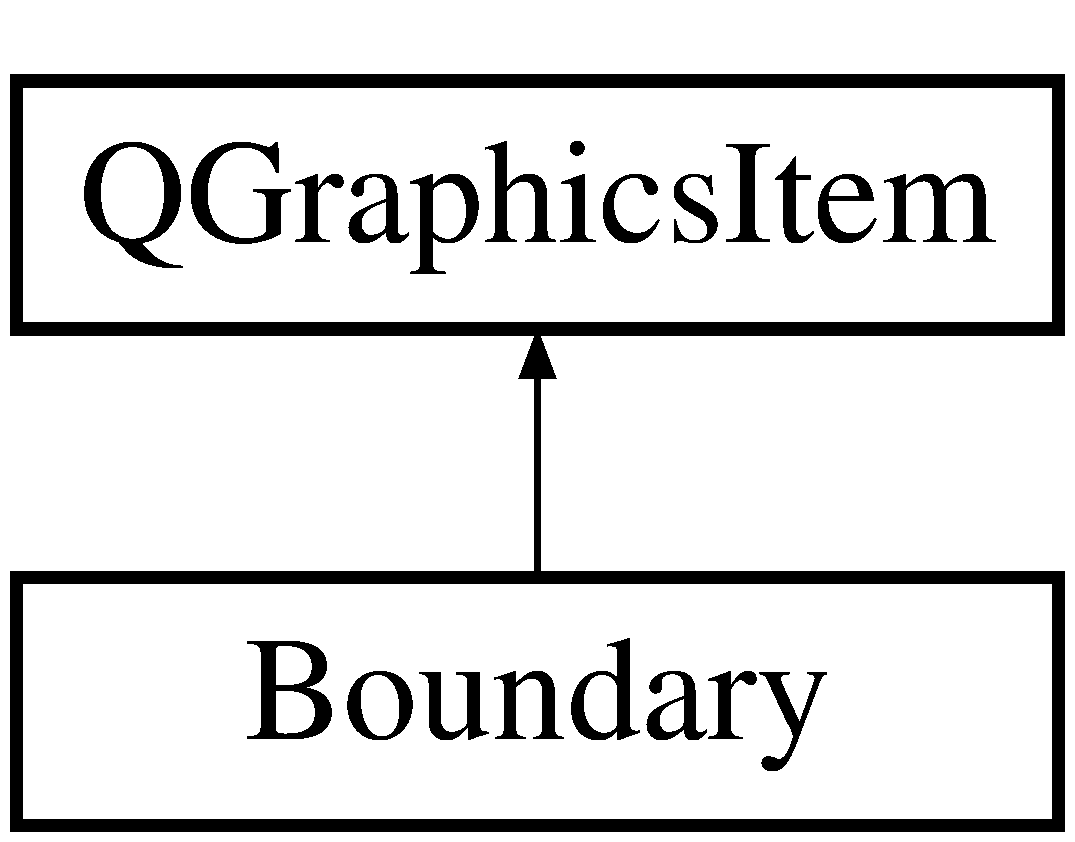
\includegraphics[height=2.000000cm]{class_boundary}
\end{center}
\end{figure}
\subsection*{Public Member Functions}
\begin{DoxyCompactItemize}
\item 
\hyperlink{class_boundary_a7c4c8db45b13dab630e4c6ed7a958e71}{Boundary} ()
\item 
Q\+Rect\+F \hyperlink{class_boundary_a91b757833c75865d1c83c3d55b65b3a9}{bounding\+Rect} () const  override
\item 
void \hyperlink{class_boundary_a248258bccc564beb94b8def8948173fb}{paint} (Q\+Painter $\ast$painter, const Q\+Style\+Option\+Graphics\+Item $\ast$option, Q\+Widget $\ast$widget=0) override
\end{DoxyCompactItemize}


\subsection{Constructor \& Destructor Documentation}
\hypertarget{class_boundary_a7c4c8db45b13dab630e4c6ed7a958e71}{}\index{Boundary@{Boundary}!Boundary@{Boundary}}
\index{Boundary@{Boundary}!Boundary@{Boundary}}
\subsubsection[{Boundary()}]{\setlength{\rightskip}{0pt plus 5cm}Boundary\+::\+Boundary (
\begin{DoxyParamCaption}
{}
\end{DoxyParamCaption}
)}\label{class_boundary_a7c4c8db45b13dab630e4c6ed7a958e71}


\subsection{Member Function Documentation}
\hypertarget{class_boundary_a91b757833c75865d1c83c3d55b65b3a9}{}\index{Boundary@{Boundary}!bounding\+Rect@{bounding\+Rect}}
\index{bounding\+Rect@{bounding\+Rect}!Boundary@{Boundary}}
\subsubsection[{bounding\+Rect() const  override}]{\setlength{\rightskip}{0pt plus 5cm}Q\+Rect\+F Boundary\+::bounding\+Rect (
\begin{DoxyParamCaption}
{}
\end{DoxyParamCaption}
) const\hspace{0.3cm}{\ttfamily [override]}}\label{class_boundary_a91b757833c75865d1c83c3d55b65b3a9}
\hypertarget{class_boundary_a248258bccc564beb94b8def8948173fb}{}\index{Boundary@{Boundary}!paint@{paint}}
\index{paint@{paint}!Boundary@{Boundary}}
\subsubsection[{paint(\+Q\+Painter $\ast$painter, const Q\+Style\+Option\+Graphics\+Item $\ast$option, Q\+Widget $\ast$widget=0) override}]{\setlength{\rightskip}{0pt plus 5cm}void Boundary\+::paint (
\begin{DoxyParamCaption}
\item[{Q\+Painter $\ast$}]{painter, }
\item[{const Q\+Style\+Option\+Graphics\+Item $\ast$}]{option, }
\item[{Q\+Widget $\ast$}]{widget = {\ttfamily 0}}
\end{DoxyParamCaption}
)\hspace{0.3cm}{\ttfamily [override]}}\label{class_boundary_a248258bccc564beb94b8def8948173fb}


The documentation for this class was generated from the following files\+:\begin{DoxyCompactItemize}
\item 
graphics/\hyperlink{_boundary_8hpp}{Boundary.\+hpp}\item 
graphics/\hyperlink{_boundary_8cpp}{Boundary.\+cpp}\end{DoxyCompactItemize}

\hypertarget{class_circle}{}\section{Circle Class Reference}
\label{class_circle}\index{Circle@{Circle}}


The \hyperlink{class_circle}{Circle} class represents an abstract circle. A circle may exist in either a hyperbolic or euclidean geometry.  




{\ttfamily \#include $<$Circle.\+hpp$>$}

Inheritance diagram for Circle\+:\begin{figure}[H]
\begin{center}
\leavevmode
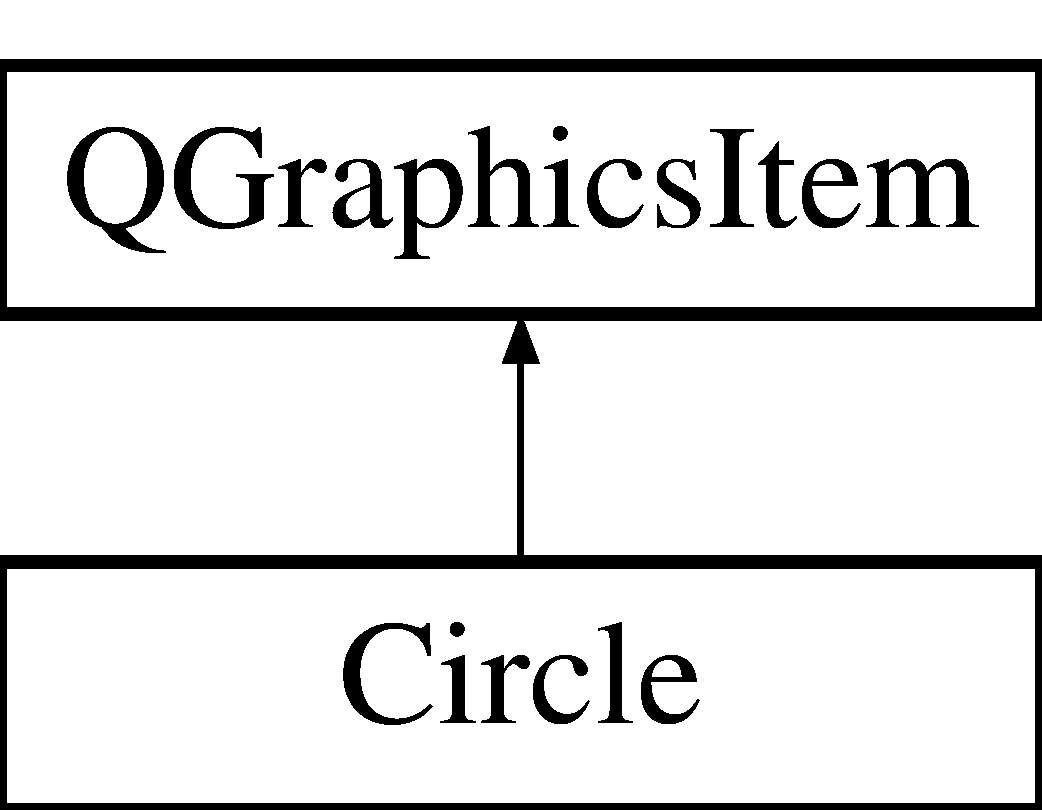
\includegraphics[height=2.000000cm]{class_circle}
\end{center}
\end{figure}
\subsection*{Public Types}
\begin{DoxyCompactItemize}
\item 
enum \hyperlink{class_circle_abaea7f437ac8e5519b3a69bce0848140}{Selection\+State} \{ \hyperlink{class_circle_abaea7f437ac8e5519b3a69bce0848140a6adf97f83acf6453d4a6a4b1070f3754}{Selection\+State\+::\+None}, 
\hyperlink{class_circle_abaea7f437ac8e5519b3a69bce0848140a91b442d385b54e1418d81adc34871053}{Selection\+State\+::\+Selected}, 
\hyperlink{class_circle_abaea7f437ac8e5519b3a69bce0848140a667b9fee30643bd8533437714aff2f69}{Selection\+State\+::\+Surrounded}
 \}
\end{DoxyCompactItemize}
\subsection*{Public Member Functions}
\begin{DoxyCompactItemize}
\item 
\hyperlink{class_circle_a868970e092a93d7b9f33e665a3f22380}{Circle} (\hyperlink{class_node}{Node} $\ast$n, \hyperlink{class_packing}{Packing} $\ast$p)
\item 
Q\+Rect\+F \hyperlink{class_circle_a00aab04a8e096d14a5a56ae1eb620275}{bounding\+Rect} () const Q\+\_\+\+D\+E\+C\+L\+\_\+\+O\+V\+E\+R\+R\+I\+D\+E
\item 
Q\+Painter\+Path \hyperlink{class_circle_a841007c456f5bc7be91b5901a7630ce3}{shape} () const Q\+\_\+\+D\+E\+C\+L\+\_\+\+O\+V\+E\+R\+R\+I\+D\+E
\item 
void \hyperlink{class_circle_a3adfe40ef373defa3e427072f00cc0a2}{paint} (Q\+Painter $\ast$painter, const Q\+Style\+Option\+Graphics\+Item $\ast$option, Q\+Widget $\ast$widget=nullptr) Q\+\_\+\+D\+E\+C\+L\+\_\+\+O\+V\+E\+R\+R\+I\+D\+E
\item 
\hyperlink{class_circle_abaea7f437ac8e5519b3a69bce0848140}{Selection\+State} \hyperlink{class_circle_af5a48f5fc296b4b84056febe3ce17a75}{get\+Selection\+State} ()
\item 
void \hyperlink{class_circle_a3a3ac6da7ed29a19f45c869b10be7a91}{set\+Selection\+State} (\hyperlink{class_circle_abaea7f437ac8e5519b3a69bce0848140}{Selection\+State} s)
\item 
\hyperlink{class_node}{Node} $\ast$ \hyperlink{class_circle_a22131e1f54de4142ed23e55902c2402c}{get\+Node} ()
\end{DoxyCompactItemize}


\subsection{Detailed Description}
The \hyperlink{class_circle}{Circle} class represents an abstract circle. A circle may exist in either a hyperbolic or euclidean geometry. 

\subsection{Member Enumeration Documentation}
\hypertarget{class_circle_abaea7f437ac8e5519b3a69bce0848140}{}\index{Circle@{Circle}!Selection\+State@{Selection\+State}}
\index{Selection\+State@{Selection\+State}!Circle@{Circle}}
\subsubsection[{Selection\+State}]{\setlength{\rightskip}{0pt plus 5cm}enum {\bf Circle\+::\+Selection\+State}\hspace{0.3cm}{\ttfamily [strong]}}\label{class_circle_abaea7f437ac8e5519b3a69bce0848140}
\begin{Desc}
\item[Enumerator]\par
\begin{description}
\index{None@{None}!Circle@{Circle}}\index{Circle@{Circle}!None@{None}}\item[{\em 
\hypertarget{class_circle_abaea7f437ac8e5519b3a69bce0848140a6adf97f83acf6453d4a6a4b1070f3754}{}None\label{class_circle_abaea7f437ac8e5519b3a69bce0848140a6adf97f83acf6453d4a6a4b1070f3754}
}]\index{Selected@{Selected}!Circle@{Circle}}\index{Circle@{Circle}!Selected@{Selected}}\item[{\em 
\hypertarget{class_circle_abaea7f437ac8e5519b3a69bce0848140a91b442d385b54e1418d81adc34871053}{}Selected\label{class_circle_abaea7f437ac8e5519b3a69bce0848140a91b442d385b54e1418d81adc34871053}
}]\index{Surrounded@{Surrounded}!Circle@{Circle}}\index{Circle@{Circle}!Surrounded@{Surrounded}}\item[{\em 
\hypertarget{class_circle_abaea7f437ac8e5519b3a69bce0848140a667b9fee30643bd8533437714aff2f69}{}Surrounded\label{class_circle_abaea7f437ac8e5519b3a69bce0848140a667b9fee30643bd8533437714aff2f69}
}]\end{description}
\end{Desc}


\subsection{Constructor \& Destructor Documentation}
\hypertarget{class_circle_a868970e092a93d7b9f33e665a3f22380}{}\index{Circle@{Circle}!Circle@{Circle}}
\index{Circle@{Circle}!Circle@{Circle}}
\subsubsection[{Circle(\+Node $\ast$n, Packing $\ast$p)}]{\setlength{\rightskip}{0pt plus 5cm}Circle\+::\+Circle (
\begin{DoxyParamCaption}
\item[{{\bf Node} $\ast$}]{n, }
\item[{{\bf Packing} $\ast$}]{p}
\end{DoxyParamCaption}
)}\label{class_circle_a868970e092a93d7b9f33e665a3f22380}


\subsection{Member Function Documentation}
\hypertarget{class_circle_a00aab04a8e096d14a5a56ae1eb620275}{}\index{Circle@{Circle}!bounding\+Rect@{bounding\+Rect}}
\index{bounding\+Rect@{bounding\+Rect}!Circle@{Circle}}
\subsubsection[{bounding\+Rect() const Q\+\_\+\+D\+E\+C\+L\+\_\+\+O\+V\+E\+R\+R\+I\+D\+E}]{\setlength{\rightskip}{0pt plus 5cm}Q\+Rect\+F Circle\+::bounding\+Rect (
\begin{DoxyParamCaption}
{}
\end{DoxyParamCaption}
) const}\label{class_circle_a00aab04a8e096d14a5a56ae1eb620275}
\hypertarget{class_circle_a22131e1f54de4142ed23e55902c2402c}{}\index{Circle@{Circle}!get\+Node@{get\+Node}}
\index{get\+Node@{get\+Node}!Circle@{Circle}}
\subsubsection[{get\+Node()}]{\setlength{\rightskip}{0pt plus 5cm}{\bf Node} $\ast$ Circle\+::get\+Node (
\begin{DoxyParamCaption}
{}
\end{DoxyParamCaption}
)}\label{class_circle_a22131e1f54de4142ed23e55902c2402c}
\hypertarget{class_circle_af5a48f5fc296b4b84056febe3ce17a75}{}\index{Circle@{Circle}!get\+Selection\+State@{get\+Selection\+State}}
\index{get\+Selection\+State@{get\+Selection\+State}!Circle@{Circle}}
\subsubsection[{get\+Selection\+State()}]{\setlength{\rightskip}{0pt plus 5cm}{\bf Circle\+::\+Selection\+State} Circle\+::get\+Selection\+State (
\begin{DoxyParamCaption}
{}
\end{DoxyParamCaption}
)}\label{class_circle_af5a48f5fc296b4b84056febe3ce17a75}
\hypertarget{class_circle_a3adfe40ef373defa3e427072f00cc0a2}{}\index{Circle@{Circle}!paint@{paint}}
\index{paint@{paint}!Circle@{Circle}}
\subsubsection[{paint(\+Q\+Painter $\ast$painter, const Q\+Style\+Option\+Graphics\+Item $\ast$option, Q\+Widget $\ast$widget=nullptr) Q\+\_\+\+D\+E\+C\+L\+\_\+\+O\+V\+E\+R\+R\+I\+D\+E}]{\setlength{\rightskip}{0pt plus 5cm}void Circle\+::paint (
\begin{DoxyParamCaption}
\item[{Q\+Painter $\ast$}]{painter, }
\item[{const Q\+Style\+Option\+Graphics\+Item $\ast$}]{option, }
\item[{Q\+Widget $\ast$}]{widget = {\ttfamily nullptr}}
\end{DoxyParamCaption}
)}\label{class_circle_a3adfe40ef373defa3e427072f00cc0a2}
\hypertarget{class_circle_a3a3ac6da7ed29a19f45c869b10be7a91}{}\index{Circle@{Circle}!set\+Selection\+State@{set\+Selection\+State}}
\index{set\+Selection\+State@{set\+Selection\+State}!Circle@{Circle}}
\subsubsection[{set\+Selection\+State(\+Selection\+State s)}]{\setlength{\rightskip}{0pt plus 5cm}void Circle\+::set\+Selection\+State (
\begin{DoxyParamCaption}
\item[{{\bf Circle\+::\+Selection\+State}}]{s}
\end{DoxyParamCaption}
)}\label{class_circle_a3a3ac6da7ed29a19f45c869b10be7a91}
\hypertarget{class_circle_a841007c456f5bc7be91b5901a7630ce3}{}\index{Circle@{Circle}!shape@{shape}}
\index{shape@{shape}!Circle@{Circle}}
\subsubsection[{shape() const Q\+\_\+\+D\+E\+C\+L\+\_\+\+O\+V\+E\+R\+R\+I\+D\+E}]{\setlength{\rightskip}{0pt plus 5cm}Q\+Painter\+Path Circle\+::shape (
\begin{DoxyParamCaption}
{}
\end{DoxyParamCaption}
) const}\label{class_circle_a841007c456f5bc7be91b5901a7630ce3}


The documentation for this class was generated from the following files\+:\begin{DoxyCompactItemize}
\item 
graphics/\hyperlink{graphics_2_circle_8hpp}{Circle.\+hpp}\item 
graphics/\hyperlink{graphics_2_circle_8cpp}{Circle.\+cpp}\end{DoxyCompactItemize}

\hypertarget{class_circles_1_1_packing_1_1_circle}{}\section{Circles\+:\+:Packing\+:\+:Circle Class Reference}
\label{class_circles_1_1_packing_1_1_circle}\index{Circles\+::\+Packing\+::\+Circle@{Circles\+::\+Packing\+::\+Circle}}


{\ttfamily \#include $<$Circle.\+hpp$>$}

Inheritance diagram for Circles\+:\+:Packing\+:\+:Circle\+:\begin{figure}[H]
\begin{center}
\leavevmode
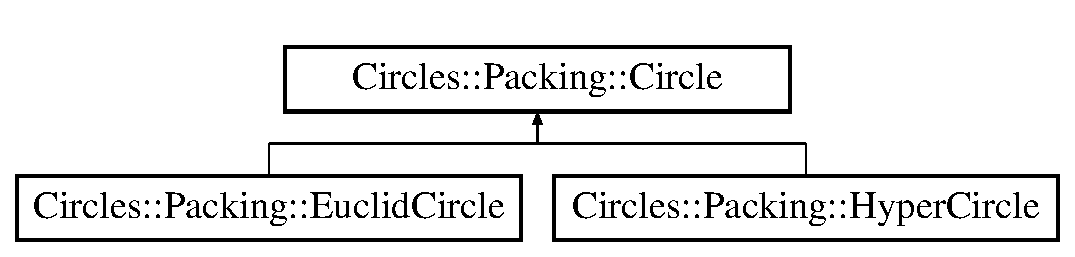
\includegraphics[height=2.000000cm]{class_circles_1_1_packing_1_1_circle}
\end{center}
\end{figure}
\subsection*{Public Member Functions}
\begin{DoxyCompactItemize}
\item 
\hyperlink{class_circles_1_1_packing_1_1_circle_ad1ecfcfc7bf34529c6a6d6c448bf70fe}{Circle} ()
\item 
int \hyperlink{class_circles_1_1_packing_1_1_circle_a426d2e69ceadbbf0d119fd117102a8a9}{index} () const 
\item 
void \hyperlink{class_circles_1_1_packing_1_1_circle_a0377f9826d119b9cbbe7abb142a66f54}{set\+Index} (int \hyperlink{class_circles_1_1_packing_1_1_circle_a426d2e69ceadbbf0d119fd117102a8a9}{index})
\item 
virtual Q\+Point\+F \hyperlink{class_circles_1_1_packing_1_1_circle_a2241ee34969d0c0266948cf1f23fa23a}{center} () const  =0
\item 
virtual qreal \hyperlink{class_circles_1_1_packing_1_1_circle_a3e34226854bcbcbd9e462e1e4fe54005}{radius} () const  =0
\item 
virtual Q\+Point\+F \hyperlink{class_circles_1_1_packing_1_1_circle_a8f410a32d3d9421231512f86fb0d564e}{proj\+Center} () const  =0
\item 
virtual qreal \hyperlink{class_circles_1_1_packing_1_1_circle_a70b927c4a58d1fe7c7576f351ce45784}{proj\+Radius} () const  =0
\item 
virtual void \hyperlink{class_circles_1_1_packing_1_1_circle_a7ed2112528b874aa2cb58854eb844b7c}{set\+Radius} (qreal r)=0
\item 
virtual bool \hyperlink{class_circles_1_1_packing_1_1_circle_a335f807f081d7f97fdea6e6d84cbc46e}{set\+Center} (Q\+Point\+F c)=0
\end{DoxyCompactItemize}
\subsection*{Protected Attributes}
\begin{DoxyCompactItemize}
\item 
int \hyperlink{class_circles_1_1_packing_1_1_circle_aaaa8e4949e8c12f7411b8f1eb9fa329c}{\+\_\+index}
\item 
qreal \hyperlink{class_circles_1_1_packing_1_1_circle_a357d2e553896a5838f871c2befcd4a5b}{\+\_\+radius}
\item 
Q\+Point\+F \hyperlink{class_circles_1_1_packing_1_1_circle_a8ea6a935ace6935eb5f5f96646f36a62}{\+\_\+center}
\end{DoxyCompactItemize}
\subsection*{Friends}
\begin{DoxyCompactItemize}
\item 
bool \hyperlink{class_circles_1_1_packing_1_1_circle_afe0b35e1a1ca89b62921b17d7400a053}{operator$<$} (const \hyperlink{class_circles_1_1_packing_1_1_circle}{Circle} \&lhs, const \hyperlink{class_circles_1_1_packing_1_1_circle}{Circle} \&rhs)
\end{DoxyCompactItemize}


\subsection{Constructor \& Destructor Documentation}
\hypertarget{class_circles_1_1_packing_1_1_circle_ad1ecfcfc7bf34529c6a6d6c448bf70fe}{}\index{Circles\+::\+Packing\+::\+Circle@{Circles\+::\+Packing\+::\+Circle}!Circle@{Circle}}
\index{Circle@{Circle}!Circles\+::\+Packing\+::\+Circle@{Circles\+::\+Packing\+::\+Circle}}
\subsubsection[{Circle()}]{\setlength{\rightskip}{0pt plus 5cm}Circle\+::\+Circle (
\begin{DoxyParamCaption}
{}
\end{DoxyParamCaption}
)}\label{class_circles_1_1_packing_1_1_circle_ad1ecfcfc7bf34529c6a6d6c448bf70fe}


\subsection{Member Function Documentation}
\hypertarget{class_circles_1_1_packing_1_1_circle_a2241ee34969d0c0266948cf1f23fa23a}{}\index{Circles\+::\+Packing\+::\+Circle@{Circles\+::\+Packing\+::\+Circle}!center@{center}}
\index{center@{center}!Circles\+::\+Packing\+::\+Circle@{Circles\+::\+Packing\+::\+Circle}}
\subsubsection[{center() const  =0}]{\setlength{\rightskip}{0pt plus 5cm}virtual Q\+Point\+F Circles\+::\+Packing\+::\+Circle\+::center (
\begin{DoxyParamCaption}
{}
\end{DoxyParamCaption}
) const\hspace{0.3cm}{\ttfamily [pure virtual]}}\label{class_circles_1_1_packing_1_1_circle_a2241ee34969d0c0266948cf1f23fa23a}
The center of the circle in it\textquotesingle{}s local space. \begin{DoxyReturn}{Returns}
The point of the center of the circle in local coordinates. 
\end{DoxyReturn}


Implemented in \hyperlink{class_circles_1_1_packing_1_1_hyper_circle_a51297723cfb8adac038a706dabbbb1e7}{Circles\+::\+Packing\+::\+Hyper\+Circle}, and \hyperlink{class_circles_1_1_packing_1_1_euclid_circle_aec7ab3f46badc0dd8d6b9eae66465435}{Circles\+::\+Packing\+::\+Euclid\+Circle}.

\hypertarget{class_circles_1_1_packing_1_1_circle_a426d2e69ceadbbf0d119fd117102a8a9}{}\index{Circles\+::\+Packing\+::\+Circle@{Circles\+::\+Packing\+::\+Circle}!index@{index}}
\index{index@{index}!Circles\+::\+Packing\+::\+Circle@{Circles\+::\+Packing\+::\+Circle}}
\subsubsection[{index() const }]{\setlength{\rightskip}{0pt plus 5cm}int Circle\+::index (
\begin{DoxyParamCaption}
{}
\end{DoxyParamCaption}
) const}\label{class_circles_1_1_packing_1_1_circle_a426d2e69ceadbbf0d119fd117102a8a9}
Get the index of the graph node associated with this \hyperlink{class_circles_1_1_packing_1_1_circle}{Circle}. \begin{DoxyReturn}{Returns}
index of the graph node. 
\end{DoxyReturn}
\hypertarget{class_circles_1_1_packing_1_1_circle_a8f410a32d3d9421231512f86fb0d564e}{}\index{Circles\+::\+Packing\+::\+Circle@{Circles\+::\+Packing\+::\+Circle}!proj\+Center@{proj\+Center}}
\index{proj\+Center@{proj\+Center}!Circles\+::\+Packing\+::\+Circle@{Circles\+::\+Packing\+::\+Circle}}
\subsubsection[{proj\+Center() const  =0}]{\setlength{\rightskip}{0pt plus 5cm}virtual Q\+Point\+F Circles\+::\+Packing\+::\+Circle\+::proj\+Center (
\begin{DoxyParamCaption}
{}
\end{DoxyParamCaption}
) const\hspace{0.3cm}{\ttfamily [pure virtual]}}\label{class_circles_1_1_packing_1_1_circle_a8f410a32d3d9421231512f86fb0d564e}
The center of the circle when projected into euclidean space (ie as it is on the monitor). For circles that exist in Euclidean space, this will be equal to its \hyperlink{class_circles_1_1_packing_1_1_circle_a2241ee34969d0c0266948cf1f23fa23a}{center()} \begin{DoxyReturn}{Returns}
the projected center of the circle. 
\end{DoxyReturn}


Implemented in \hyperlink{class_circles_1_1_packing_1_1_hyper_circle_a4a00caa714bc479d2b7d777c7cf41b19}{Circles\+::\+Packing\+::\+Hyper\+Circle}, and \hyperlink{class_circles_1_1_packing_1_1_euclid_circle_a4444a4bab157bee09e7dddf89b026d18}{Circles\+::\+Packing\+::\+Euclid\+Circle}.

\hypertarget{class_circles_1_1_packing_1_1_circle_a70b927c4a58d1fe7c7576f351ce45784}{}\index{Circles\+::\+Packing\+::\+Circle@{Circles\+::\+Packing\+::\+Circle}!proj\+Radius@{proj\+Radius}}
\index{proj\+Radius@{proj\+Radius}!Circles\+::\+Packing\+::\+Circle@{Circles\+::\+Packing\+::\+Circle}}
\subsubsection[{proj\+Radius() const  =0}]{\setlength{\rightskip}{0pt plus 5cm}virtual qreal Circles\+::\+Packing\+::\+Circle\+::proj\+Radius (
\begin{DoxyParamCaption}
{}
\end{DoxyParamCaption}
) const\hspace{0.3cm}{\ttfamily [pure virtual]}}\label{class_circles_1_1_packing_1_1_circle_a70b927c4a58d1fe7c7576f351ce45784}
The radius of the circle when projected into euclidean space (ie as it is on the monitor). For circles that exist in Euclidean space, this will be equal to its \hyperlink{class_circles_1_1_packing_1_1_circle_a3e34226854bcbcbd9e462e1e4fe54005}{radius()}. \begin{DoxyReturn}{Returns}
the projected radius of the circle. 
\end{DoxyReturn}


Implemented in \hyperlink{class_circles_1_1_packing_1_1_hyper_circle_aee965a2f67ebf52e9cf88b2eb6f53b9f}{Circles\+::\+Packing\+::\+Hyper\+Circle}, and \hyperlink{class_circles_1_1_packing_1_1_euclid_circle_a3c22ce28f6ede8bba1346523a3800c3b}{Circles\+::\+Packing\+::\+Euclid\+Circle}.

\hypertarget{class_circles_1_1_packing_1_1_circle_a3e34226854bcbcbd9e462e1e4fe54005}{}\index{Circles\+::\+Packing\+::\+Circle@{Circles\+::\+Packing\+::\+Circle}!radius@{radius}}
\index{radius@{radius}!Circles\+::\+Packing\+::\+Circle@{Circles\+::\+Packing\+::\+Circle}}
\subsubsection[{radius() const  =0}]{\setlength{\rightskip}{0pt plus 5cm}virtual qreal Circles\+::\+Packing\+::\+Circle\+::radius (
\begin{DoxyParamCaption}
{}
\end{DoxyParamCaption}
) const\hspace{0.3cm}{\ttfamily [pure virtual]}}\label{class_circles_1_1_packing_1_1_circle_a3e34226854bcbcbd9e462e1e4fe54005}
The radius of the circle in its local space. \begin{DoxyReturn}{Returns}
radius of the circle in its local space. 
\end{DoxyReturn}


Implemented in \hyperlink{class_circles_1_1_packing_1_1_hyper_circle_a6d841473a2de1967aea00933f31400ed}{Circles\+::\+Packing\+::\+Hyper\+Circle}, and \hyperlink{class_circles_1_1_packing_1_1_euclid_circle_af34ecb130884f976ecb5849463d60dbb}{Circles\+::\+Packing\+::\+Euclid\+Circle}.

\hypertarget{class_circles_1_1_packing_1_1_circle_a335f807f081d7f97fdea6e6d84cbc46e}{}\index{Circles\+::\+Packing\+::\+Circle@{Circles\+::\+Packing\+::\+Circle}!set\+Center@{set\+Center}}
\index{set\+Center@{set\+Center}!Circles\+::\+Packing\+::\+Circle@{Circles\+::\+Packing\+::\+Circle}}
\subsubsection[{set\+Center(\+Q\+Point\+F c)=0}]{\setlength{\rightskip}{0pt plus 5cm}virtual bool Circles\+::\+Packing\+::\+Circle\+::set\+Center (
\begin{DoxyParamCaption}
\item[{Q\+Point\+F}]{c}
\end{DoxyParamCaption}
)\hspace{0.3cm}{\ttfamily [pure virtual]}}\label{class_circles_1_1_packing_1_1_circle_a335f807f081d7f97fdea6e6d84cbc46e}
Attempt to set the center of the circle. 
\begin{DoxyParams}{Parameters}
{\em c} & the center to set \\
\hline
\end{DoxyParams}
\begin{DoxyReturn}{Returns}
True if the center was set correctly. False otherwise. 
\end{DoxyReturn}


Implemented in \hyperlink{class_circles_1_1_packing_1_1_hyper_circle_a5c4e09db77fee96d649d3faba1ee0a76}{Circles\+::\+Packing\+::\+Hyper\+Circle}, and \hyperlink{class_circles_1_1_packing_1_1_euclid_circle_a9186f704f10ecfb53a1ca2dba148c092}{Circles\+::\+Packing\+::\+Euclid\+Circle}.

\hypertarget{class_circles_1_1_packing_1_1_circle_a0377f9826d119b9cbbe7abb142a66f54}{}\index{Circles\+::\+Packing\+::\+Circle@{Circles\+::\+Packing\+::\+Circle}!set\+Index@{set\+Index}}
\index{set\+Index@{set\+Index}!Circles\+::\+Packing\+::\+Circle@{Circles\+::\+Packing\+::\+Circle}}
\subsubsection[{set\+Index(int index)}]{\setlength{\rightskip}{0pt plus 5cm}void Circle\+::set\+Index (
\begin{DoxyParamCaption}
\item[{int}]{index}
\end{DoxyParamCaption}
)}\label{class_circles_1_1_packing_1_1_circle_a0377f9826d119b9cbbe7abb142a66f54}
Set the index of this circle 
\begin{DoxyParams}{Parameters}
{\em index} & the index of the associated node in the graph. \\
\hline
\end{DoxyParams}
\hypertarget{class_circles_1_1_packing_1_1_circle_a7ed2112528b874aa2cb58854eb844b7c}{}\index{Circles\+::\+Packing\+::\+Circle@{Circles\+::\+Packing\+::\+Circle}!set\+Radius@{set\+Radius}}
\index{set\+Radius@{set\+Radius}!Circles\+::\+Packing\+::\+Circle@{Circles\+::\+Packing\+::\+Circle}}
\subsubsection[{set\+Radius(qreal r)=0}]{\setlength{\rightskip}{0pt plus 5cm}virtual void Circles\+::\+Packing\+::\+Circle\+::set\+Radius (
\begin{DoxyParamCaption}
\item[{qreal}]{r}
\end{DoxyParamCaption}
)\hspace{0.3cm}{\ttfamily [pure virtual]}}\label{class_circles_1_1_packing_1_1_circle_a7ed2112528b874aa2cb58854eb844b7c}
Set the radius of the circle to the specified value. 
\begin{DoxyParams}{Parameters}
{\em r} & The new radius of the circle. (in local space) \\
\hline
\end{DoxyParams}


Implemented in \hyperlink{class_circles_1_1_packing_1_1_hyper_circle_a615257ea4d789aae5641fafca8c49047}{Circles\+::\+Packing\+::\+Hyper\+Circle}, and \hyperlink{class_circles_1_1_packing_1_1_euclid_circle_a648a838ba8dd501dbe10e8304349dbb4}{Circles\+::\+Packing\+::\+Euclid\+Circle}.



\subsection{Friends And Related Function Documentation}
\hypertarget{class_circles_1_1_packing_1_1_circle_afe0b35e1a1ca89b62921b17d7400a053}{}\index{Circles\+::\+Packing\+::\+Circle@{Circles\+::\+Packing\+::\+Circle}!operator$<$@{operator$<$}}
\index{operator$<$@{operator$<$}!Circles\+::\+Packing\+::\+Circle@{Circles\+::\+Packing\+::\+Circle}}
\subsubsection[{operator$<$}]{\setlength{\rightskip}{0pt plus 5cm}bool operator$<$ (
\begin{DoxyParamCaption}
\item[{const {\bf Circle} \&}]{lhs, }
\item[{const {\bf Circle} \&}]{rhs}
\end{DoxyParamCaption}
)\hspace{0.3cm}{\ttfamily [friend]}}\label{class_circles_1_1_packing_1_1_circle_afe0b35e1a1ca89b62921b17d7400a053}
Order comparison for sorting in lists, etc. 
\begin{DoxyParams}{Parameters}
{\em lhs} & \\
\hline
{\em rhs} & \\
\hline
\end{DoxyParams}
\begin{DoxyReturn}{Returns}

\end{DoxyReturn}


\subsection{Member Data Documentation}
\hypertarget{class_circles_1_1_packing_1_1_circle_a8ea6a935ace6935eb5f5f96646f36a62}{}\index{Circles\+::\+Packing\+::\+Circle@{Circles\+::\+Packing\+::\+Circle}!\+\_\+center@{\+\_\+center}}
\index{\+\_\+center@{\+\_\+center}!Circles\+::\+Packing\+::\+Circle@{Circles\+::\+Packing\+::\+Circle}}
\subsubsection[{\+\_\+center}]{\setlength{\rightskip}{0pt plus 5cm}Q\+Point\+F Circles\+::\+Packing\+::\+Circle\+::\+\_\+center\hspace{0.3cm}{\ttfamily [protected]}}\label{class_circles_1_1_packing_1_1_circle_a8ea6a935ace6935eb5f5f96646f36a62}
\hypertarget{class_circles_1_1_packing_1_1_circle_aaaa8e4949e8c12f7411b8f1eb9fa329c}{}\index{Circles\+::\+Packing\+::\+Circle@{Circles\+::\+Packing\+::\+Circle}!\+\_\+index@{\+\_\+index}}
\index{\+\_\+index@{\+\_\+index}!Circles\+::\+Packing\+::\+Circle@{Circles\+::\+Packing\+::\+Circle}}
\subsubsection[{\+\_\+index}]{\setlength{\rightskip}{0pt plus 5cm}int Circles\+::\+Packing\+::\+Circle\+::\+\_\+index\hspace{0.3cm}{\ttfamily [protected]}}\label{class_circles_1_1_packing_1_1_circle_aaaa8e4949e8c12f7411b8f1eb9fa329c}
\hypertarget{class_circles_1_1_packing_1_1_circle_a357d2e553896a5838f871c2befcd4a5b}{}\index{Circles\+::\+Packing\+::\+Circle@{Circles\+::\+Packing\+::\+Circle}!\+\_\+radius@{\+\_\+radius}}
\index{\+\_\+radius@{\+\_\+radius}!Circles\+::\+Packing\+::\+Circle@{Circles\+::\+Packing\+::\+Circle}}
\subsubsection[{\+\_\+radius}]{\setlength{\rightskip}{0pt plus 5cm}qreal Circles\+::\+Packing\+::\+Circle\+::\+\_\+radius\hspace{0.3cm}{\ttfamily [protected]}}\label{class_circles_1_1_packing_1_1_circle_a357d2e553896a5838f871c2befcd4a5b}


The documentation for this class was generated from the following files\+:\begin{DoxyCompactItemize}
\item 
packing/\hyperlink{packing_2_circle_8hpp}{Circle.\+hpp}\item 
packing/\hyperlink{packing_2_circle_8cpp}{Circle.\+cpp}\end{DoxyCompactItemize}

\hypertarget{class_connector}{}\section{Connector Class Reference}
\label{class_connector}\index{Connector@{Connector}}


{\ttfamily \#include $<$Connector.\+hpp$>$}

Inheritance diagram for Connector\+:\begin{figure}[H]
\begin{center}
\leavevmode
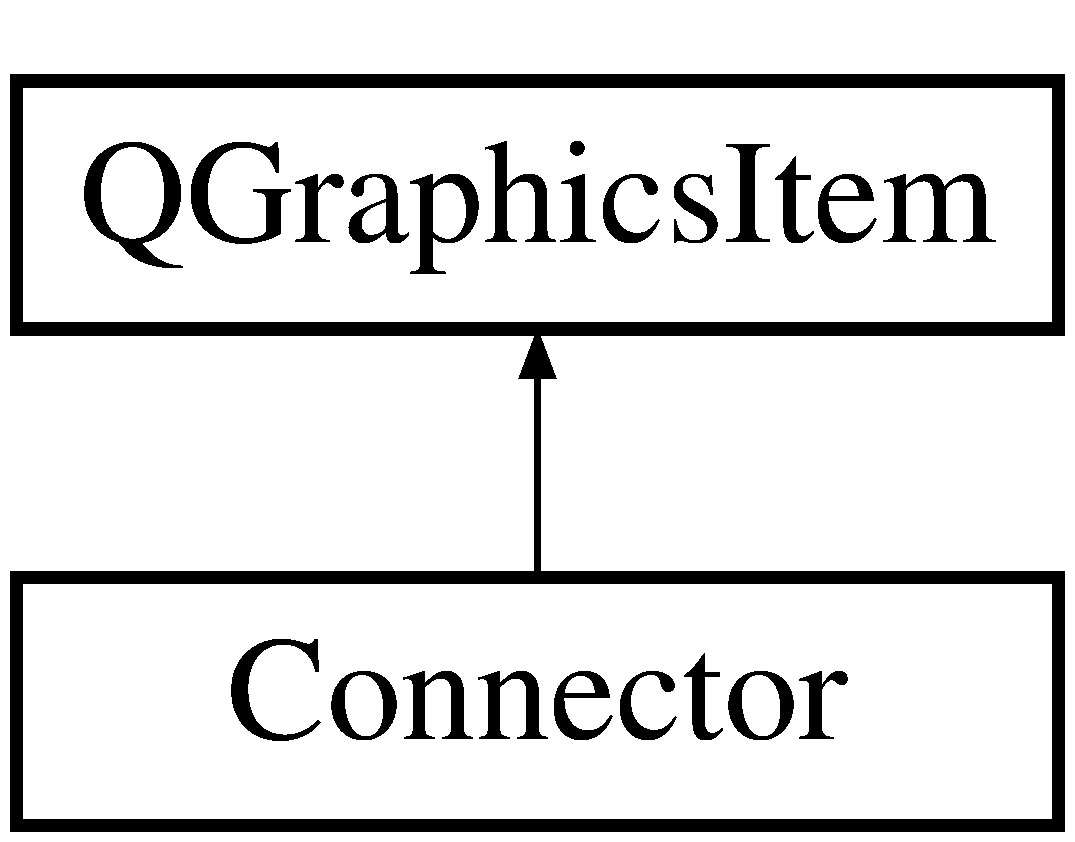
\includegraphics[height=2.000000cm]{class_connector}
\end{center}
\end{figure}
\subsection*{Public Member Functions}
\begin{DoxyCompactItemize}
\item 
\hyperlink{class_connector_a039a739b61255d9645f355920bff91c4}{Connector} (\hyperlink{class_node}{Node} $\ast$n1, \hyperlink{class_node}{Node} $\ast$n2)
\item 
Q\+Rect\+F \hyperlink{class_connector_a43883a193fe80ccbd6f5cbe3a8d5f955}{bounding\+Rect} () const Q\+\_\+\+D\+E\+C\+L\+\_\+\+O\+V\+E\+R\+R\+I\+D\+E
\item 
void \hyperlink{class_connector_a76a81524aa51aefff7885ea989b1f0f4}{paint} (Q\+Painter $\ast$painter, const Q\+Style\+Option\+Graphics\+Item $\ast$option, Q\+Widget $\ast$widget=nullptr) Q\+\_\+\+D\+E\+C\+L\+\_\+\+O\+V\+E\+R\+R\+I\+D\+E
\end{DoxyCompactItemize}


\subsection{Constructor \& Destructor Documentation}
\hypertarget{class_connector_a039a739b61255d9645f355920bff91c4}{}\index{Connector@{Connector}!Connector@{Connector}}
\index{Connector@{Connector}!Connector@{Connector}}
\subsubsection[{Connector(\+Node $\ast$n1, Node $\ast$n2)}]{\setlength{\rightskip}{0pt plus 5cm}Connector\+::\+Connector (
\begin{DoxyParamCaption}
\item[{{\bf Node} $\ast$}]{n1, }
\item[{{\bf Node} $\ast$}]{n2}
\end{DoxyParamCaption}
)}\label{class_connector_a039a739b61255d9645f355920bff91c4}


\subsection{Member Function Documentation}
\hypertarget{class_connector_a43883a193fe80ccbd6f5cbe3a8d5f955}{}\index{Connector@{Connector}!bounding\+Rect@{bounding\+Rect}}
\index{bounding\+Rect@{bounding\+Rect}!Connector@{Connector}}
\subsubsection[{bounding\+Rect() const Q\+\_\+\+D\+E\+C\+L\+\_\+\+O\+V\+E\+R\+R\+I\+D\+E}]{\setlength{\rightskip}{0pt plus 5cm}Q\+Rect\+F Connector\+::bounding\+Rect (
\begin{DoxyParamCaption}
{}
\end{DoxyParamCaption}
) const}\label{class_connector_a43883a193fe80ccbd6f5cbe3a8d5f955}
\hypertarget{class_connector_a76a81524aa51aefff7885ea989b1f0f4}{}\index{Connector@{Connector}!paint@{paint}}
\index{paint@{paint}!Connector@{Connector}}
\subsubsection[{paint(\+Q\+Painter $\ast$painter, const Q\+Style\+Option\+Graphics\+Item $\ast$option, Q\+Widget $\ast$widget=nullptr) Q\+\_\+\+D\+E\+C\+L\+\_\+\+O\+V\+E\+R\+R\+I\+D\+E}]{\setlength{\rightskip}{0pt plus 5cm}void Connector\+::paint (
\begin{DoxyParamCaption}
\item[{Q\+Painter $\ast$}]{painter, }
\item[{const Q\+Style\+Option\+Graphics\+Item $\ast$}]{option, }
\item[{Q\+Widget $\ast$}]{widget = {\ttfamily nullptr}}
\end{DoxyParamCaption}
)}\label{class_connector_a76a81524aa51aefff7885ea989b1f0f4}


The documentation for this class was generated from the following files\+:\begin{DoxyCompactItemize}
\item 
graphics/\hyperlink{_connector_8hpp}{Connector.\+hpp}\item 
graphics/\hyperlink{_connector_8cpp}{Connector.\+cpp}\end{DoxyCompactItemize}

\hypertarget{class_circles_1_1_graph_1_1_edge}{}\section{Circles\+:\+:Graph\+:\+:Edge Class Reference}
\label{class_circles_1_1_graph_1_1_edge}\index{Circles\+::\+Graph\+::\+Edge@{Circles\+::\+Graph\+::\+Edge}}


{\ttfamily \#include $<$Edge.\+hpp$>$}

\subsection*{Public Member Functions}
\begin{DoxyCompactItemize}
\item 
\hyperlink{class_circles_1_1_graph_1_1_edge_a1216aca8c410cc6015b3c7f5499a99ef}{Edge} ()
\item 
\hyperlink{class_circles_1_1_graph_1_1_edge_ae785946b2536c47df4e38218b19794ea}{Edge} (int x, int y)
\item 
\hyperlink{class_circles_1_1_graph_1_1_edge_a84861f7ebd4da01b4943b640a57550c7}{Edge} (const \hyperlink{class_circles_1_1_graph_1_1_edge}{Edge} \&other)
\item 
\hyperlink{class_circles_1_1_graph_1_1_edge}{Edge} \& \hyperlink{class_circles_1_1_graph_1_1_edge_adddfd55ecff7af40a77b875472033e65}{operator=} (const \hyperlink{class_circles_1_1_graph_1_1_edge}{Edge} \&other)
\item 
int \hyperlink{class_circles_1_1_graph_1_1_edge_a90aa10d5676780244ba7878a0eb004c5}{get\+X} ()
\item 
int \hyperlink{class_circles_1_1_graph_1_1_edge_a4f17f350f047c1c43a580d139054c9ee}{get\+Y} ()
\item 
void \hyperlink{class_circles_1_1_graph_1_1_edge_a4c92864bb8878fd0719d5d500a6bc41a}{set\+X} (int x)
\item 
void \hyperlink{class_circles_1_1_graph_1_1_edge_a90f019d37e3c756b6092c7aecd0fe02c}{set\+Y} (int y)
\item 
void \hyperlink{class_circles_1_1_graph_1_1_edge_a41770bfce297232513138848812f703c}{set} (int x, int y)
\end{DoxyCompactItemize}
\subsection*{Friends}
\begin{DoxyCompactItemize}
\item 
bool \hyperlink{class_circles_1_1_graph_1_1_edge_a8c214bf5445e306ca857f50670e54578}{operator==} (const \hyperlink{class_circles_1_1_graph_1_1_edge}{Edge} \&lhs, const \hyperlink{class_circles_1_1_graph_1_1_edge}{Edge} \&rhs)
\end{DoxyCompactItemize}


\subsection{Detailed Description}
Defines an edge between two nodes in a graph. An edge is defined by the two nodes that it is co-\/incident to. The two defining nodes are constrained so that the lower-\/order one is the first argument. 

\subsection{Constructor \& Destructor Documentation}
\hypertarget{class_circles_1_1_graph_1_1_edge_a1216aca8c410cc6015b3c7f5499a99ef}{}\index{Circles\+::\+Graph\+::\+Edge@{Circles\+::\+Graph\+::\+Edge}!Edge@{Edge}}
\index{Edge@{Edge}!Circles\+::\+Graph\+::\+Edge@{Circles\+::\+Graph\+::\+Edge}}
\subsubsection[{Edge()}]{\setlength{\rightskip}{0pt plus 5cm}Circles\+::\+Graph\+::\+Edge\+::\+Edge (
\begin{DoxyParamCaption}
{}
\end{DoxyParamCaption}
)}\label{class_circles_1_1_graph_1_1_edge_a1216aca8c410cc6015b3c7f5499a99ef}
Default constructor. Initializes the edge to (-\/1, -\/1) \hypertarget{class_circles_1_1_graph_1_1_edge_ae785946b2536c47df4e38218b19794ea}{}\index{Circles\+::\+Graph\+::\+Edge@{Circles\+::\+Graph\+::\+Edge}!Edge@{Edge}}
\index{Edge@{Edge}!Circles\+::\+Graph\+::\+Edge@{Circles\+::\+Graph\+::\+Edge}}
\subsubsection[{Edge(int x, int y)}]{\setlength{\rightskip}{0pt plus 5cm}Circles\+::\+Graph\+::\+Edge\+::\+Edge (
\begin{DoxyParamCaption}
\item[{int}]{x, }
\item[{int}]{y}
\end{DoxyParamCaption}
)}\label{class_circles_1_1_graph_1_1_edge_ae785946b2536c47df4e38218b19794ea}
Construct an edge. The first node should be lower-\/order than the second. 
\begin{DoxyParams}{Parameters}
{\em x} & index of the first node of the edge \\
\hline
{\em y} & index of the second node of the edge. \\
\hline
\end{DoxyParams}
\hypertarget{class_circles_1_1_graph_1_1_edge_a84861f7ebd4da01b4943b640a57550c7}{}\index{Circles\+::\+Graph\+::\+Edge@{Circles\+::\+Graph\+::\+Edge}!Edge@{Edge}}
\index{Edge@{Edge}!Circles\+::\+Graph\+::\+Edge@{Circles\+::\+Graph\+::\+Edge}}
\subsubsection[{Edge(const Edge \&other)}]{\setlength{\rightskip}{0pt plus 5cm}Circles\+::\+Graph\+::\+Edge\+::\+Edge (
\begin{DoxyParamCaption}
\item[{const {\bf Edge} \&}]{other}
\end{DoxyParamCaption}
)}\label{class_circles_1_1_graph_1_1_edge_a84861f7ebd4da01b4943b640a57550c7}


\subsection{Member Function Documentation}
\hypertarget{class_circles_1_1_graph_1_1_edge_a90aa10d5676780244ba7878a0eb004c5}{}\index{Circles\+::\+Graph\+::\+Edge@{Circles\+::\+Graph\+::\+Edge}!get\+X@{get\+X}}
\index{get\+X@{get\+X}!Circles\+::\+Graph\+::\+Edge@{Circles\+::\+Graph\+::\+Edge}}
\subsubsection[{get\+X()}]{\setlength{\rightskip}{0pt plus 5cm}int Circles\+::\+Graph\+::\+Edge\+::get\+X (
\begin{DoxyParamCaption}
{}
\end{DoxyParamCaption}
)}\label{class_circles_1_1_graph_1_1_edge_a90aa10d5676780244ba7878a0eb004c5}
\hypertarget{class_circles_1_1_graph_1_1_edge_a4f17f350f047c1c43a580d139054c9ee}{}\index{Circles\+::\+Graph\+::\+Edge@{Circles\+::\+Graph\+::\+Edge}!get\+Y@{get\+Y}}
\index{get\+Y@{get\+Y}!Circles\+::\+Graph\+::\+Edge@{Circles\+::\+Graph\+::\+Edge}}
\subsubsection[{get\+Y()}]{\setlength{\rightskip}{0pt plus 5cm}int Circles\+::\+Graph\+::\+Edge\+::get\+Y (
\begin{DoxyParamCaption}
{}
\end{DoxyParamCaption}
)}\label{class_circles_1_1_graph_1_1_edge_a4f17f350f047c1c43a580d139054c9ee}
\hypertarget{class_circles_1_1_graph_1_1_edge_adddfd55ecff7af40a77b875472033e65}{}\index{Circles\+::\+Graph\+::\+Edge@{Circles\+::\+Graph\+::\+Edge}!operator=@{operator=}}
\index{operator=@{operator=}!Circles\+::\+Graph\+::\+Edge@{Circles\+::\+Graph\+::\+Edge}}
\subsubsection[{operator=(const Edge \&other)}]{\setlength{\rightskip}{0pt plus 5cm}{\bf Edge} \& Circles\+::\+Graph\+::\+Edge\+::operator= (
\begin{DoxyParamCaption}
\item[{const {\bf Edge} \&}]{other}
\end{DoxyParamCaption}
)}\label{class_circles_1_1_graph_1_1_edge_adddfd55ecff7af40a77b875472033e65}
\hypertarget{class_circles_1_1_graph_1_1_edge_a41770bfce297232513138848812f703c}{}\index{Circles\+::\+Graph\+::\+Edge@{Circles\+::\+Graph\+::\+Edge}!set@{set}}
\index{set@{set}!Circles\+::\+Graph\+::\+Edge@{Circles\+::\+Graph\+::\+Edge}}
\subsubsection[{set(int x, int y)}]{\setlength{\rightskip}{0pt plus 5cm}void Circles\+::\+Graph\+::\+Edge\+::set (
\begin{DoxyParamCaption}
\item[{int}]{x, }
\item[{int}]{y}
\end{DoxyParamCaption}
)}\label{class_circles_1_1_graph_1_1_edge_a41770bfce297232513138848812f703c}
\hypertarget{class_circles_1_1_graph_1_1_edge_a4c92864bb8878fd0719d5d500a6bc41a}{}\index{Circles\+::\+Graph\+::\+Edge@{Circles\+::\+Graph\+::\+Edge}!set\+X@{set\+X}}
\index{set\+X@{set\+X}!Circles\+::\+Graph\+::\+Edge@{Circles\+::\+Graph\+::\+Edge}}
\subsubsection[{set\+X(int x)}]{\setlength{\rightskip}{0pt plus 5cm}void Circles\+::\+Graph\+::\+Edge\+::set\+X (
\begin{DoxyParamCaption}
\item[{int}]{x}
\end{DoxyParamCaption}
)}\label{class_circles_1_1_graph_1_1_edge_a4c92864bb8878fd0719d5d500a6bc41a}
\hypertarget{class_circles_1_1_graph_1_1_edge_a90f019d37e3c756b6092c7aecd0fe02c}{}\index{Circles\+::\+Graph\+::\+Edge@{Circles\+::\+Graph\+::\+Edge}!set\+Y@{set\+Y}}
\index{set\+Y@{set\+Y}!Circles\+::\+Graph\+::\+Edge@{Circles\+::\+Graph\+::\+Edge}}
\subsubsection[{set\+Y(int y)}]{\setlength{\rightskip}{0pt plus 5cm}void Circles\+::\+Graph\+::\+Edge\+::set\+Y (
\begin{DoxyParamCaption}
\item[{int}]{y}
\end{DoxyParamCaption}
)}\label{class_circles_1_1_graph_1_1_edge_a90f019d37e3c756b6092c7aecd0fe02c}


\subsection{Friends And Related Function Documentation}
\hypertarget{class_circles_1_1_graph_1_1_edge_a8c214bf5445e306ca857f50670e54578}{}\index{Circles\+::\+Graph\+::\+Edge@{Circles\+::\+Graph\+::\+Edge}!operator==@{operator==}}
\index{operator==@{operator==}!Circles\+::\+Graph\+::\+Edge@{Circles\+::\+Graph\+::\+Edge}}
\subsubsection[{operator==}]{\setlength{\rightskip}{0pt plus 5cm}bool operator== (
\begin{DoxyParamCaption}
\item[{const {\bf Edge} \&}]{lhs, }
\item[{const {\bf Edge} \&}]{rhs}
\end{DoxyParamCaption}
)\hspace{0.3cm}{\ttfamily [friend]}}\label{class_circles_1_1_graph_1_1_edge_a8c214bf5445e306ca857f50670e54578}


The documentation for this class was generated from the following files\+:\begin{DoxyCompactItemize}
\item 
graph/\hyperlink{_edge_8hpp}{Edge.\+hpp}\item 
graph/\hyperlink{_edge_8cpp}{Edge.\+cpp}\end{DoxyCompactItemize}

\hypertarget{class_circles_1_1_packing_1_1_euclid_circle}{}\section{Circles\+:\+:Packing\+:\+:Euclid\+Circle Class Reference}
\label{class_circles_1_1_packing_1_1_euclid_circle}\index{Circles\+::\+Packing\+::\+Euclid\+Circle@{Circles\+::\+Packing\+::\+Euclid\+Circle}}


{\ttfamily \#include $<$Euclid\+Circle.\+hpp$>$}

Inheritance diagram for Circles\+:\+:Packing\+:\+:Euclid\+Circle\+:\begin{figure}[H]
\begin{center}
\leavevmode
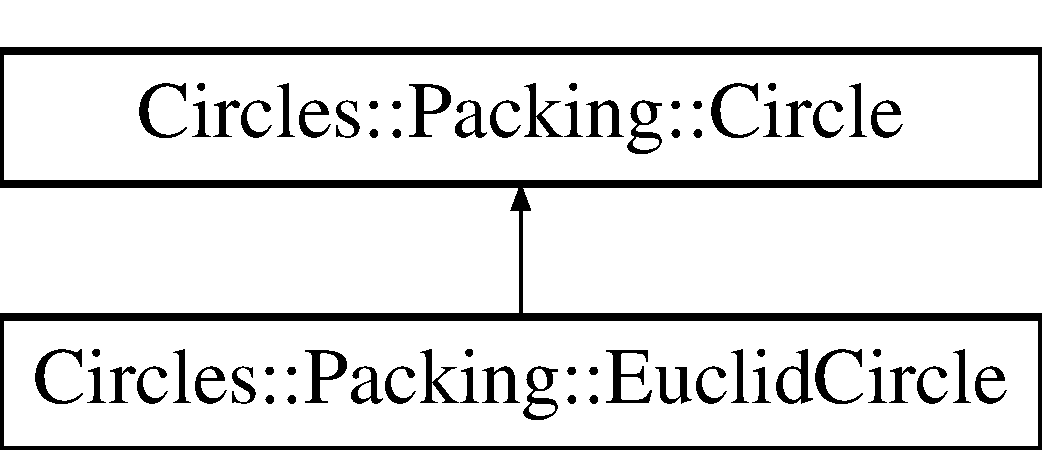
\includegraphics[height=2.000000cm]{class_circles_1_1_packing_1_1_euclid_circle}
\end{center}
\end{figure}
\subsection*{Public Member Functions}
\begin{DoxyCompactItemize}
\item 
\hyperlink{class_circles_1_1_packing_1_1_euclid_circle_a20844fd3b36876330de35a7b135d6c1d}{Euclid\+Circle} ()
\item 
\hyperlink{class_circles_1_1_packing_1_1_euclid_circle_ab82afcad97df0d08ba78a3aa679aa16f}{Euclid\+Circle} (const Q\+Point\+F \&\hyperlink{class_circles_1_1_packing_1_1_euclid_circle_aec7ab3f46badc0dd8d6b9eae66465435}{center}, qreal \hyperlink{class_circles_1_1_packing_1_1_euclid_circle_af34ecb130884f976ecb5849463d60dbb}{radius}, int \hyperlink{class_circles_1_1_packing_1_1_circle_a426d2e69ceadbbf0d119fd117102a8a9}{index})
\item 
\hyperlink{class_circles_1_1_packing_1_1_euclid_circle_ab850e2caabe2edcc75229546af893740}{Euclid\+Circle} (const \hyperlink{class_circles_1_1_packing_1_1_euclid_circle}{Euclid\+Circle} \&other)
\item 
\hyperlink{class_circles_1_1_packing_1_1_euclid_circle}{Euclid\+Circle} \& \hyperlink{class_circles_1_1_packing_1_1_euclid_circle_ada694a1cf8517ffb437b8d9f224827c1}{operator=} (const \hyperlink{class_circles_1_1_packing_1_1_euclid_circle}{Euclid\+Circle} \&other)
\item 
virtual Q\+Point\+F \hyperlink{class_circles_1_1_packing_1_1_euclid_circle_aec7ab3f46badc0dd8d6b9eae66465435}{center} () const  override
\item 
virtual qreal \hyperlink{class_circles_1_1_packing_1_1_euclid_circle_af34ecb130884f976ecb5849463d60dbb}{radius} () const  override
\item 
virtual Q\+Point\+F \hyperlink{class_circles_1_1_packing_1_1_euclid_circle_a4444a4bab157bee09e7dddf89b026d18}{proj\+Center} () const  override
\item 
virtual qreal \hyperlink{class_circles_1_1_packing_1_1_euclid_circle_a3c22ce28f6ede8bba1346523a3800c3b}{proj\+Radius} () const  override
\item 
virtual void \hyperlink{class_circles_1_1_packing_1_1_euclid_circle_a648a838ba8dd501dbe10e8304349dbb4}{set\+Radius} (qreal r) override
\item 
virtual bool \hyperlink{class_circles_1_1_packing_1_1_euclid_circle_a9186f704f10ecfb53a1ca2dba148c092}{set\+Center} (Q\+Point\+F c) override
\end{DoxyCompactItemize}
\subsection*{Friends}
\begin{DoxyCompactItemize}
\item 
bool \hyperlink{class_circles_1_1_packing_1_1_euclid_circle_af3bfd627199cc10af703c37d3daad3ea}{operator==} (const \hyperlink{class_circles_1_1_packing_1_1_euclid_circle}{Euclid\+Circle} \&lhs, const \hyperlink{class_circles_1_1_packing_1_1_euclid_circle}{Euclid\+Circle} \&rhs)
\end{DoxyCompactItemize}
\subsection*{Additional Inherited Members}


\subsection{Detailed Description}
A circle on the euclidean plane. 

\subsection{Constructor \& Destructor Documentation}
\hypertarget{class_circles_1_1_packing_1_1_euclid_circle_a20844fd3b36876330de35a7b135d6c1d}{}\index{Circles\+::\+Packing\+::\+Euclid\+Circle@{Circles\+::\+Packing\+::\+Euclid\+Circle}!Euclid\+Circle@{Euclid\+Circle}}
\index{Euclid\+Circle@{Euclid\+Circle}!Circles\+::\+Packing\+::\+Euclid\+Circle@{Circles\+::\+Packing\+::\+Euclid\+Circle}}
\subsubsection[{Euclid\+Circle()}]{\setlength{\rightskip}{0pt plus 5cm}Circles\+::\+Packing\+::\+Euclid\+Circle\+::\+Euclid\+Circle (
\begin{DoxyParamCaption}
{}
\end{DoxyParamCaption}
)}\label{class_circles_1_1_packing_1_1_euclid_circle_a20844fd3b36876330de35a7b135d6c1d}
Construct an empty euclidean circle, centered at (0, 0) with radius 1.\+0, and index -\/1. \hypertarget{class_circles_1_1_packing_1_1_euclid_circle_ab82afcad97df0d08ba78a3aa679aa16f}{}\index{Circles\+::\+Packing\+::\+Euclid\+Circle@{Circles\+::\+Packing\+::\+Euclid\+Circle}!Euclid\+Circle@{Euclid\+Circle}}
\index{Euclid\+Circle@{Euclid\+Circle}!Circles\+::\+Packing\+::\+Euclid\+Circle@{Circles\+::\+Packing\+::\+Euclid\+Circle}}
\subsubsection[{Euclid\+Circle(const Q\+Point\+F \&center, qreal radius, int index)}]{\setlength{\rightskip}{0pt plus 5cm}Circles\+::\+Packing\+::\+Euclid\+Circle\+::\+Euclid\+Circle (
\begin{DoxyParamCaption}
\item[{const Q\+Point\+F \&}]{center, }
\item[{qreal}]{radius, }
\item[{int}]{index}
\end{DoxyParamCaption}
)}\label{class_circles_1_1_packing_1_1_euclid_circle_ab82afcad97df0d08ba78a3aa679aa16f}
Construct a euclidean circle with a given center , radius, and index. 
\begin{DoxyParams}{Parameters}
{\em center} & Center point of the circle, in euclidean space. \\
\hline
{\em radius} & Radius of the circle. \\
\hline
{\em index} & Index of corresponding node in the underlying graph. \\
\hline
\end{DoxyParams}
\hypertarget{class_circles_1_1_packing_1_1_euclid_circle_ab850e2caabe2edcc75229546af893740}{}\index{Circles\+::\+Packing\+::\+Euclid\+Circle@{Circles\+::\+Packing\+::\+Euclid\+Circle}!Euclid\+Circle@{Euclid\+Circle}}
\index{Euclid\+Circle@{Euclid\+Circle}!Circles\+::\+Packing\+::\+Euclid\+Circle@{Circles\+::\+Packing\+::\+Euclid\+Circle}}
\subsubsection[{Euclid\+Circle(const Euclid\+Circle \&other)}]{\setlength{\rightskip}{0pt plus 5cm}Circles\+::\+Packing\+::\+Euclid\+Circle\+::\+Euclid\+Circle (
\begin{DoxyParamCaption}
\item[{const {\bf Euclid\+Circle} \&}]{other}
\end{DoxyParamCaption}
)}\label{class_circles_1_1_packing_1_1_euclid_circle_ab850e2caabe2edcc75229546af893740}


\subsection{Member Function Documentation}
\hypertarget{class_circles_1_1_packing_1_1_euclid_circle_aec7ab3f46badc0dd8d6b9eae66465435}{}\index{Circles\+::\+Packing\+::\+Euclid\+Circle@{Circles\+::\+Packing\+::\+Euclid\+Circle}!center@{center}}
\index{center@{center}!Circles\+::\+Packing\+::\+Euclid\+Circle@{Circles\+::\+Packing\+::\+Euclid\+Circle}}
\subsubsection[{center() const  override}]{\setlength{\rightskip}{0pt plus 5cm}Q\+Point\+F Circles\+::\+Packing\+::\+Euclid\+Circle\+::center (
\begin{DoxyParamCaption}
{}
\end{DoxyParamCaption}
) const\hspace{0.3cm}{\ttfamily [override]}, {\ttfamily [virtual]}}\label{class_circles_1_1_packing_1_1_euclid_circle_aec7ab3f46badc0dd8d6b9eae66465435}
The center of the circle in it\textquotesingle{}s local space. \begin{DoxyReturn}{Returns}
The point of the center of the circle in local coordinates. 
\end{DoxyReturn}


Implements \hyperlink{class_circles_1_1_packing_1_1_circle_a2241ee34969d0c0266948cf1f23fa23a}{Circles\+::\+Packing\+::\+Circle}.

\hypertarget{class_circles_1_1_packing_1_1_euclid_circle_ada694a1cf8517ffb437b8d9f224827c1}{}\index{Circles\+::\+Packing\+::\+Euclid\+Circle@{Circles\+::\+Packing\+::\+Euclid\+Circle}!operator=@{operator=}}
\index{operator=@{operator=}!Circles\+::\+Packing\+::\+Euclid\+Circle@{Circles\+::\+Packing\+::\+Euclid\+Circle}}
\subsubsection[{operator=(const Euclid\+Circle \&other)}]{\setlength{\rightskip}{0pt plus 5cm}{\bf Euclid\+Circle} \& Circles\+::\+Packing\+::\+Euclid\+Circle\+::operator= (
\begin{DoxyParamCaption}
\item[{const {\bf Euclid\+Circle} \&}]{other}
\end{DoxyParamCaption}
)}\label{class_circles_1_1_packing_1_1_euclid_circle_ada694a1cf8517ffb437b8d9f224827c1}
\hypertarget{class_circles_1_1_packing_1_1_euclid_circle_a4444a4bab157bee09e7dddf89b026d18}{}\index{Circles\+::\+Packing\+::\+Euclid\+Circle@{Circles\+::\+Packing\+::\+Euclid\+Circle}!proj\+Center@{proj\+Center}}
\index{proj\+Center@{proj\+Center}!Circles\+::\+Packing\+::\+Euclid\+Circle@{Circles\+::\+Packing\+::\+Euclid\+Circle}}
\subsubsection[{proj\+Center() const  override}]{\setlength{\rightskip}{0pt plus 5cm}Q\+Point\+F Circles\+::\+Packing\+::\+Euclid\+Circle\+::proj\+Center (
\begin{DoxyParamCaption}
{}
\end{DoxyParamCaption}
) const\hspace{0.3cm}{\ttfamily [override]}, {\ttfamily [virtual]}}\label{class_circles_1_1_packing_1_1_euclid_circle_a4444a4bab157bee09e7dddf89b026d18}
The center of the circle when projected into euclidean space (ie as it is on the monitor). For circles that exist in Euclidean space, this will be equal to its \hyperlink{class_circles_1_1_packing_1_1_euclid_circle_aec7ab3f46badc0dd8d6b9eae66465435}{center()} \begin{DoxyReturn}{Returns}
the projected center of the circle. 
\end{DoxyReturn}


Implements \hyperlink{class_circles_1_1_packing_1_1_circle_a8f410a32d3d9421231512f86fb0d564e}{Circles\+::\+Packing\+::\+Circle}.

\hypertarget{class_circles_1_1_packing_1_1_euclid_circle_a3c22ce28f6ede8bba1346523a3800c3b}{}\index{Circles\+::\+Packing\+::\+Euclid\+Circle@{Circles\+::\+Packing\+::\+Euclid\+Circle}!proj\+Radius@{proj\+Radius}}
\index{proj\+Radius@{proj\+Radius}!Circles\+::\+Packing\+::\+Euclid\+Circle@{Circles\+::\+Packing\+::\+Euclid\+Circle}}
\subsubsection[{proj\+Radius() const  override}]{\setlength{\rightskip}{0pt plus 5cm}qreal Circles\+::\+Packing\+::\+Euclid\+Circle\+::proj\+Radius (
\begin{DoxyParamCaption}
{}
\end{DoxyParamCaption}
) const\hspace{0.3cm}{\ttfamily [override]}, {\ttfamily [virtual]}}\label{class_circles_1_1_packing_1_1_euclid_circle_a3c22ce28f6ede8bba1346523a3800c3b}
The radius of the circle when projected into euclidean space (ie as it is on the monitor). For circles that exist in Euclidean space, this will be equal to its \hyperlink{class_circles_1_1_packing_1_1_euclid_circle_af34ecb130884f976ecb5849463d60dbb}{radius()}. \begin{DoxyReturn}{Returns}
the projected radius of the circle. 
\end{DoxyReturn}


Implements \hyperlink{class_circles_1_1_packing_1_1_circle_a70b927c4a58d1fe7c7576f351ce45784}{Circles\+::\+Packing\+::\+Circle}.

\hypertarget{class_circles_1_1_packing_1_1_euclid_circle_af34ecb130884f976ecb5849463d60dbb}{}\index{Circles\+::\+Packing\+::\+Euclid\+Circle@{Circles\+::\+Packing\+::\+Euclid\+Circle}!radius@{radius}}
\index{radius@{radius}!Circles\+::\+Packing\+::\+Euclid\+Circle@{Circles\+::\+Packing\+::\+Euclid\+Circle}}
\subsubsection[{radius() const  override}]{\setlength{\rightskip}{0pt plus 5cm}qreal Circles\+::\+Packing\+::\+Euclid\+Circle\+::radius (
\begin{DoxyParamCaption}
{}
\end{DoxyParamCaption}
) const\hspace{0.3cm}{\ttfamily [override]}, {\ttfamily [virtual]}}\label{class_circles_1_1_packing_1_1_euclid_circle_af34ecb130884f976ecb5849463d60dbb}
The radius of the circle in its local space. \begin{DoxyReturn}{Returns}
radius of the circle in its local space. 
\end{DoxyReturn}


Implements \hyperlink{class_circles_1_1_packing_1_1_circle_a3e34226854bcbcbd9e462e1e4fe54005}{Circles\+::\+Packing\+::\+Circle}.

\hypertarget{class_circles_1_1_packing_1_1_euclid_circle_a9186f704f10ecfb53a1ca2dba148c092}{}\index{Circles\+::\+Packing\+::\+Euclid\+Circle@{Circles\+::\+Packing\+::\+Euclid\+Circle}!set\+Center@{set\+Center}}
\index{set\+Center@{set\+Center}!Circles\+::\+Packing\+::\+Euclid\+Circle@{Circles\+::\+Packing\+::\+Euclid\+Circle}}
\subsubsection[{set\+Center(\+Q\+Point\+F c) override}]{\setlength{\rightskip}{0pt plus 5cm}bool Circles\+::\+Packing\+::\+Euclid\+Circle\+::set\+Center (
\begin{DoxyParamCaption}
\item[{Q\+Point\+F}]{c}
\end{DoxyParamCaption}
)\hspace{0.3cm}{\ttfamily [override]}, {\ttfamily [virtual]}}\label{class_circles_1_1_packing_1_1_euclid_circle_a9186f704f10ecfb53a1ca2dba148c092}
Attempt to set the center of the circle. 
\begin{DoxyParams}{Parameters}
{\em c} & the center to set \\
\hline
\end{DoxyParams}
\begin{DoxyReturn}{Returns}
True if the center was set correctly. False otherwise. 
\end{DoxyReturn}


Implements \hyperlink{class_circles_1_1_packing_1_1_circle_a335f807f081d7f97fdea6e6d84cbc46e}{Circles\+::\+Packing\+::\+Circle}.

\hypertarget{class_circles_1_1_packing_1_1_euclid_circle_a648a838ba8dd501dbe10e8304349dbb4}{}\index{Circles\+::\+Packing\+::\+Euclid\+Circle@{Circles\+::\+Packing\+::\+Euclid\+Circle}!set\+Radius@{set\+Radius}}
\index{set\+Radius@{set\+Radius}!Circles\+::\+Packing\+::\+Euclid\+Circle@{Circles\+::\+Packing\+::\+Euclid\+Circle}}
\subsubsection[{set\+Radius(qreal r) override}]{\setlength{\rightskip}{0pt plus 5cm}void Circles\+::\+Packing\+::\+Euclid\+Circle\+::set\+Radius (
\begin{DoxyParamCaption}
\item[{qreal}]{r}
\end{DoxyParamCaption}
)\hspace{0.3cm}{\ttfamily [override]}, {\ttfamily [virtual]}}\label{class_circles_1_1_packing_1_1_euclid_circle_a648a838ba8dd501dbe10e8304349dbb4}
Set the radius of the circle to the specified value. 
\begin{DoxyParams}{Parameters}
{\em r} & The new radius of the circle. (in local space) \\
\hline
\end{DoxyParams}


Implements \hyperlink{class_circles_1_1_packing_1_1_circle_a7ed2112528b874aa2cb58854eb844b7c}{Circles\+::\+Packing\+::\+Circle}.



\subsection{Friends And Related Function Documentation}
\hypertarget{class_circles_1_1_packing_1_1_euclid_circle_af3bfd627199cc10af703c37d3daad3ea}{}\index{Circles\+::\+Packing\+::\+Euclid\+Circle@{Circles\+::\+Packing\+::\+Euclid\+Circle}!operator==@{operator==}}
\index{operator==@{operator==}!Circles\+::\+Packing\+::\+Euclid\+Circle@{Circles\+::\+Packing\+::\+Euclid\+Circle}}
\subsubsection[{operator==}]{\setlength{\rightskip}{0pt plus 5cm}bool operator== (
\begin{DoxyParamCaption}
\item[{const {\bf Euclid\+Circle} \&}]{lhs, }
\item[{const {\bf Euclid\+Circle} \&}]{rhs}
\end{DoxyParamCaption}
)\hspace{0.3cm}{\ttfamily [friend]}}\label{class_circles_1_1_packing_1_1_euclid_circle_af3bfd627199cc10af703c37d3daad3ea}


The documentation for this class was generated from the following files\+:\begin{DoxyCompactItemize}
\item 
packing/\hyperlink{_euclid_circle_8hpp}{Euclid\+Circle.\+hpp}\item 
packing/\hyperlink{_euclid_circle_8cpp}{Euclid\+Circle.\+cpp}\end{DoxyCompactItemize}

\hypertarget{class_circles_1_1_packing_1_1_euclid_packing}{}\section{Circles\+:\+:Packing\+:\+:Euclid\+Packing Class Reference}
\label{class_circles_1_1_packing_1_1_euclid_packing}\index{Circles\+::\+Packing\+::\+Euclid\+Packing@{Circles\+::\+Packing\+::\+Euclid\+Packing}}


{\ttfamily \#include $<$Euclid\+Packing.\+hpp$>$}

Inheritance diagram for Circles\+:\+:Packing\+:\+:Euclid\+Packing\+:\begin{figure}[H]
\begin{center}
\leavevmode
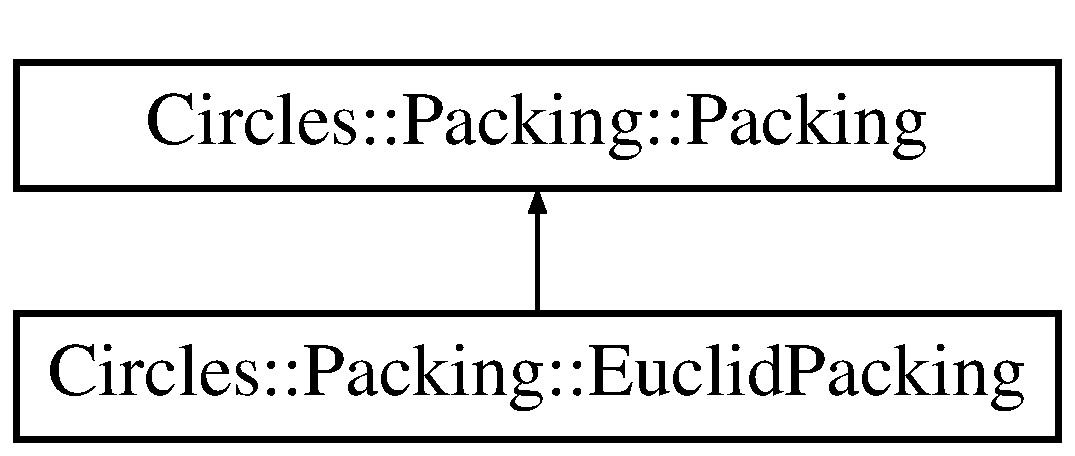
\includegraphics[height=2.000000cm]{class_circles_1_1_packing_1_1_euclid_packing}
\end{center}
\end{figure}
\subsection*{Public Member Functions}
\begin{DoxyCompactItemize}
\item 
\hyperlink{class_circles_1_1_packing_1_1_euclid_packing_a5db8505818c5a58c8e37e501813f4b69}{Euclid\+Packing} ()
\item 
\hyperlink{class_circles_1_1_packing_1_1_euclid_packing_a23f5455e15a83f88cad6c5e79a495eb9}{Euclid\+Packing} (std\+::shared\+\_\+ptr$<$ \hyperlink{class_circles_1_1_graph_1_1_graph}{Graph\+::\+Graph} $>$ g)
\item 
\hyperlink{class_circles_1_1_packing_1_1_euclid_packing_a731f170953bccf905bcb12e79571a76f}{Euclid\+Packing} (std\+::shared\+\_\+ptr$<$ \hyperlink{class_circles_1_1_graph_1_1_graph}{Graph\+::\+Graph} $>$ g, const Q\+List$<$ \hyperlink{class_circles_1_1_packing_1_1_circle}{Circle} $\ast$ $>$ \&\hyperlink{class_circles_1_1_packing_1_1_packing_a6dec25e7a0fc0fee6e1f3fb7856a7867}{circles})
\item 
\hyperlink{class_circles_1_1_packing_1_1_euclid_packing_a7babfff0f6b3390ed698483a08dd97bf}{Euclid\+Packing} (const \hyperlink{class_circles_1_1_packing_1_1_euclid_packing}{Euclid\+Packing} \&other)
\item 
\hyperlink{class_circles_1_1_packing_1_1_euclid_packing_acf4e49f672ff5293b1c30d44637ea114}{Euclid\+Packing} (\hyperlink{class_circles_1_1_packing_1_1_euclid_packing}{Euclid\+Packing} \&\&other)
\item 
\hyperlink{class_circles_1_1_packing_1_1_euclid_packing}{Euclid\+Packing} \& \hyperlink{class_circles_1_1_packing_1_1_euclid_packing_a279dd7eadfe7bdd3a0186e5fd9a4a21e}{operator=} (const \hyperlink{class_circles_1_1_packing_1_1_euclid_packing}{Euclid\+Packing} \&other)
\item 
\hyperlink{class_circles_1_1_packing_1_1_euclid_packing}{Euclid\+Packing} \& \hyperlink{class_circles_1_1_packing_1_1_euclid_packing_ab4cb93514eb1f813c04ac86211948180}{operator=} (\hyperlink{class_circles_1_1_packing_1_1_euclid_packing}{Euclid\+Packing} \&\&other)
\end{DoxyCompactItemize}
\subsection*{Friends}
\begin{DoxyCompactItemize}
\item 
bool \hyperlink{class_circles_1_1_packing_1_1_euclid_packing_a26518eba9f5ed05fae7a39f5fe7c6f41}{operator==} (const \hyperlink{class_circles_1_1_packing_1_1_euclid_packing}{Euclid\+Packing} \&lhs, const \hyperlink{class_circles_1_1_packing_1_1_euclid_packing}{Euclid\+Packing} \&rhs)
\end{DoxyCompactItemize}
\subsection*{Additional Inherited Members}


\subsection{Detailed Description}
A packing on the euclidean plane. Holds Euclid\+Circles. 

\subsection{Constructor \& Destructor Documentation}
\hypertarget{class_circles_1_1_packing_1_1_euclid_packing_a5db8505818c5a58c8e37e501813f4b69}{}\index{Circles\+::\+Packing\+::\+Euclid\+Packing@{Circles\+::\+Packing\+::\+Euclid\+Packing}!Euclid\+Packing@{Euclid\+Packing}}
\index{Euclid\+Packing@{Euclid\+Packing}!Circles\+::\+Packing\+::\+Euclid\+Packing@{Circles\+::\+Packing\+::\+Euclid\+Packing}}
\subsubsection[{Euclid\+Packing()}]{\setlength{\rightskip}{0pt plus 5cm}Euclid\+Packing\+::\+Euclid\+Packing (
\begin{DoxyParamCaption}
{}
\end{DoxyParamCaption}
)}\label{class_circles_1_1_packing_1_1_euclid_packing_a5db8505818c5a58c8e37e501813f4b69}
Construct an empty packing with no underlying graph. (don\textquotesingle{}t use this) \hypertarget{class_circles_1_1_packing_1_1_euclid_packing_a23f5455e15a83f88cad6c5e79a495eb9}{}\index{Circles\+::\+Packing\+::\+Euclid\+Packing@{Circles\+::\+Packing\+::\+Euclid\+Packing}!Euclid\+Packing@{Euclid\+Packing}}
\index{Euclid\+Packing@{Euclid\+Packing}!Circles\+::\+Packing\+::\+Euclid\+Packing@{Circles\+::\+Packing\+::\+Euclid\+Packing}}
\subsubsection[{Euclid\+Packing(std\+::shared\+\_\+ptr$<$ Graph\+::\+Graph $>$ g)}]{\setlength{\rightskip}{0pt plus 5cm}Circles\+::\+Packing\+::\+Euclid\+Packing\+::\+Euclid\+Packing (
\begin{DoxyParamCaption}
\item[{std\+::shared\+\_\+ptr$<$ {\bf Graph\+::\+Graph} $>$}]{g}
\end{DoxyParamCaption}
)}\label{class_circles_1_1_packing_1_1_euclid_packing_a23f5455e15a83f88cad6c5e79a495eb9}
Construct a new euclidean packing with a specified underlying graph. All circles will be initialized to radius 1 and center 0,0. 
\begin{DoxyParams}{Parameters}
{\em g} & pointer to underlying graph. \\
\hline
\end{DoxyParams}
\hypertarget{class_circles_1_1_packing_1_1_euclid_packing_a731f170953bccf905bcb12e79571a76f}{}\index{Circles\+::\+Packing\+::\+Euclid\+Packing@{Circles\+::\+Packing\+::\+Euclid\+Packing}!Euclid\+Packing@{Euclid\+Packing}}
\index{Euclid\+Packing@{Euclid\+Packing}!Circles\+::\+Packing\+::\+Euclid\+Packing@{Circles\+::\+Packing\+::\+Euclid\+Packing}}
\subsubsection[{Euclid\+Packing(std\+::shared\+\_\+ptr$<$ Graph\+::\+Graph $>$ g, const Q\+List$<$ Circle $\ast$ $>$ \&circles)}]{\setlength{\rightskip}{0pt plus 5cm}Circles\+::\+Packing\+::\+Euclid\+Packing\+::\+Euclid\+Packing (
\begin{DoxyParamCaption}
\item[{std\+::shared\+\_\+ptr$<$ {\bf Graph\+::\+Graph} $>$}]{g, }
\item[{const Q\+List$<$ {\bf Circle} $\ast$ $>$ \&}]{circles}
\end{DoxyParamCaption}
)}\label{class_circles_1_1_packing_1_1_euclid_packing_a731f170953bccf905bcb12e79571a76f}
Construct a new euclidean packing with a specified underlying graph and pre-\/defined circles. 
\begin{DoxyParams}{Parameters}
{\em g} & the underlying graph. \\
\hline
{\em circles} & List of circles to pre-\/setup. Dupliecate circles and circles which do not correspond to nodes present in the graph will be removed. Any nodes without circles in the list will have their circles initialized to radius 1.\+0 and center 0,0. \\
\hline
\end{DoxyParams}
\hypertarget{class_circles_1_1_packing_1_1_euclid_packing_a7babfff0f6b3390ed698483a08dd97bf}{}\index{Circles\+::\+Packing\+::\+Euclid\+Packing@{Circles\+::\+Packing\+::\+Euclid\+Packing}!Euclid\+Packing@{Euclid\+Packing}}
\index{Euclid\+Packing@{Euclid\+Packing}!Circles\+::\+Packing\+::\+Euclid\+Packing@{Circles\+::\+Packing\+::\+Euclid\+Packing}}
\subsubsection[{Euclid\+Packing(const Euclid\+Packing \&other)}]{\setlength{\rightskip}{0pt plus 5cm}Circles\+::\+Packing\+::\+Euclid\+Packing\+::\+Euclid\+Packing (
\begin{DoxyParamCaption}
\item[{const {\bf Euclid\+Packing} \&}]{other}
\end{DoxyParamCaption}
)}\label{class_circles_1_1_packing_1_1_euclid_packing_a7babfff0f6b3390ed698483a08dd97bf}
Copy reference to node as well as deep-\/copy of circles. \hypertarget{class_circles_1_1_packing_1_1_euclid_packing_acf4e49f672ff5293b1c30d44637ea114}{}\index{Circles\+::\+Packing\+::\+Euclid\+Packing@{Circles\+::\+Packing\+::\+Euclid\+Packing}!Euclid\+Packing@{Euclid\+Packing}}
\index{Euclid\+Packing@{Euclid\+Packing}!Circles\+::\+Packing\+::\+Euclid\+Packing@{Circles\+::\+Packing\+::\+Euclid\+Packing}}
\subsubsection[{Euclid\+Packing(\+Euclid\+Packing \&\&other)}]{\setlength{\rightskip}{0pt plus 5cm}Circles\+::\+Packing\+::\+Euclid\+Packing\+::\+Euclid\+Packing (
\begin{DoxyParamCaption}
\item[{{\bf Euclid\+Packing} \&\&}]{other}
\end{DoxyParamCaption}
)}\label{class_circles_1_1_packing_1_1_euclid_packing_acf4e49f672ff5293b1c30d44637ea114}


\subsection{Member Function Documentation}
\hypertarget{class_circles_1_1_packing_1_1_euclid_packing_a279dd7eadfe7bdd3a0186e5fd9a4a21e}{}\index{Circles\+::\+Packing\+::\+Euclid\+Packing@{Circles\+::\+Packing\+::\+Euclid\+Packing}!operator=@{operator=}}
\index{operator=@{operator=}!Circles\+::\+Packing\+::\+Euclid\+Packing@{Circles\+::\+Packing\+::\+Euclid\+Packing}}
\subsubsection[{operator=(const Euclid\+Packing \&other)}]{\setlength{\rightskip}{0pt plus 5cm}{\bf Euclid\+Packing}\& Circles\+::\+Packing\+::\+Euclid\+Packing\+::operator= (
\begin{DoxyParamCaption}
\item[{const {\bf Euclid\+Packing} \&}]{other}
\end{DoxyParamCaption}
)}\label{class_circles_1_1_packing_1_1_euclid_packing_a279dd7eadfe7bdd3a0186e5fd9a4a21e}
\hypertarget{class_circles_1_1_packing_1_1_euclid_packing_ab4cb93514eb1f813c04ac86211948180}{}\index{Circles\+::\+Packing\+::\+Euclid\+Packing@{Circles\+::\+Packing\+::\+Euclid\+Packing}!operator=@{operator=}}
\index{operator=@{operator=}!Circles\+::\+Packing\+::\+Euclid\+Packing@{Circles\+::\+Packing\+::\+Euclid\+Packing}}
\subsubsection[{operator=(\+Euclid\+Packing \&\&other)}]{\setlength{\rightskip}{0pt plus 5cm}{\bf Euclid\+Packing}\& Circles\+::\+Packing\+::\+Euclid\+Packing\+::operator= (
\begin{DoxyParamCaption}
\item[{{\bf Euclid\+Packing} \&\&}]{other}
\end{DoxyParamCaption}
)}\label{class_circles_1_1_packing_1_1_euclid_packing_ab4cb93514eb1f813c04ac86211948180}


\subsection{Friends And Related Function Documentation}
\hypertarget{class_circles_1_1_packing_1_1_euclid_packing_a26518eba9f5ed05fae7a39f5fe7c6f41}{}\index{Circles\+::\+Packing\+::\+Euclid\+Packing@{Circles\+::\+Packing\+::\+Euclid\+Packing}!operator==@{operator==}}
\index{operator==@{operator==}!Circles\+::\+Packing\+::\+Euclid\+Packing@{Circles\+::\+Packing\+::\+Euclid\+Packing}}
\subsubsection[{operator==}]{\setlength{\rightskip}{0pt plus 5cm}bool operator== (
\begin{DoxyParamCaption}
\item[{const {\bf Euclid\+Packing} \&}]{lhs, }
\item[{const {\bf Euclid\+Packing} \&}]{rhs}
\end{DoxyParamCaption}
)\hspace{0.3cm}{\ttfamily [friend]}}\label{class_circles_1_1_packing_1_1_euclid_packing_a26518eba9f5ed05fae7a39f5fe7c6f41}


The documentation for this class was generated from the following files\+:\begin{DoxyCompactItemize}
\item 
packing/\hyperlink{_euclid_packing_8hpp}{Euclid\+Packing.\+hpp}\item 
packing/\hyperlink{_euclid_packing_8cpp}{Euclid\+Packing.\+cpp}\end{DoxyCompactItemize}

\hypertarget{class_circles_1_1_graph_1_1_graph}{}\section{Circles\+:\+:Graph\+:\+:Graph Class Reference}
\label{class_circles_1_1_graph_1_1_graph}\index{Circles\+::\+Graph\+::\+Graph@{Circles\+::\+Graph\+::\+Graph}}


{\ttfamily \#include $<$Graph.\+hpp$>$}

\subsection*{Public Member Functions}
\begin{DoxyCompactItemize}
\item 
\hyperlink{class_circles_1_1_graph_1_1_graph_a95707c8bcb3a2726554f46e53e3ed81c}{Graph} ()
\item 
\hyperlink{class_circles_1_1_graph_1_1_graph_af168837b8090fde8bec04ad7655f7198}{Graph} (const \hyperlink{class_circles_1_1_graph_1_1_graph}{Graph} \&other)
\item 
\hyperlink{class_circles_1_1_graph_1_1_graph_a4e3802ce745621050d878577cc0aa3f4}{Graph} (\hyperlink{class_circles_1_1_graph_1_1_graph}{Graph} \&\&other)
\item 
\hyperlink{class_circles_1_1_graph_1_1_graph}{Graph} \& \hyperlink{class_circles_1_1_graph_1_1_graph_ae60d35a5fa5840a19e26cfd907a04c46}{operator=} (const \hyperlink{class_circles_1_1_graph_1_1_graph}{Graph} \&other)
\item 
\hyperlink{class_circles_1_1_graph_1_1_graph}{Graph} \& \hyperlink{class_circles_1_1_graph_1_1_graph_a04ed0665e13e73f64217b1d4be604cbc}{operator=} (\hyperlink{class_circles_1_1_graph_1_1_graph}{Graph} \&\&other)
\item 
void \hyperlink{class_circles_1_1_graph_1_1_graph_a82638c54c3a88927f2cd25eef5b9d3ed}{add\+Edge} (\hyperlink{namespace_circles_1_1_graph_afab3817d1ee8e2074e82866c27a1058b}{Node} x, \hyperlink{namespace_circles_1_1_graph_afab3817d1ee8e2074e82866c27a1058b}{Node} y)
\item 
void \hyperlink{class_circles_1_1_graph_1_1_graph_a32639ee46ddea3aac13fd2d14c975b8e}{add\+Edge} (\hyperlink{class_circles_1_1_graph_1_1_edge}{Edge} e)
\item 
void \hyperlink{class_circles_1_1_graph_1_1_graph_a239c35f73a0d73d1281f38f447aeb66a}{remove\+Edge} (\hyperlink{namespace_circles_1_1_graph_afab3817d1ee8e2074e82866c27a1058b}{Node} x, \hyperlink{namespace_circles_1_1_graph_afab3817d1ee8e2074e82866c27a1058b}{Node} y)
\item 
bool \hyperlink{class_circles_1_1_graph_1_1_graph_a55aa662170f9aff4e5daad2632b18801}{has\+Edge} (\hyperlink{namespace_circles_1_1_graph_afab3817d1ee8e2074e82866c27a1058b}{Node} x, \hyperlink{namespace_circles_1_1_graph_afab3817d1ee8e2074e82866c27a1058b}{Node} y) const 
\item 
bool \hyperlink{class_circles_1_1_graph_1_1_graph_ab867cc2c06fb7625e8225f7ea16696a3}{has\+Full\+Flower} (\hyperlink{namespace_circles_1_1_graph_afab3817d1ee8e2074e82866c27a1058b}{Node} n)
\item 
bool \hyperlink{class_circles_1_1_graph_1_1_graph_aba67c754b516f960cb66aeb229a05cb2}{is\+Boundary} (\hyperlink{namespace_circles_1_1_graph_afab3817d1ee8e2074e82866c27a1058b}{Node} n)
\item 
std\+::unique\+\_\+ptr$<$ Q\+List$<$ \hyperlink{namespace_circles_1_1_graph_afab3817d1ee8e2074e82866c27a1058b}{Node} $>$ $>$ \hyperlink{class_circles_1_1_graph_1_1_graph_a6e3b6554943c973fecd2f7e8244f86bb}{get\+Nodes} () const 
\item 
std\+::unique\+\_\+ptr$<$ Q\+List$<$ \hyperlink{class_circles_1_1_graph_1_1_edge}{Edge} $>$ $>$ \hyperlink{class_circles_1_1_graph_1_1_graph_adb0a409de3b4c11758fa7a0de35b9ae7}{get\+Edges} () const 
\item 
Q\+List$<$ \hyperlink{namespace_circles_1_1_graph_afab3817d1ee8e2074e82866c27a1058b}{Node} $>$ \& \hyperlink{class_circles_1_1_graph_1_1_graph_a990cfc808909eaba08c991e1113ac88c}{neighbours} (\hyperlink{namespace_circles_1_1_graph_afab3817d1ee8e2074e82866c27a1058b}{Node} i) const 
\item 
Q\+List$<$ \hyperlink{namespace_circles_1_1_graph_afab3817d1ee8e2074e82866c27a1058b}{Node} $>$ \& \hyperlink{class_circles_1_1_graph_1_1_graph_ac60eea4288fccbc6127d8f05fe8eaadf}{sorted\+Neighbours} (\hyperlink{namespace_circles_1_1_graph_afab3817d1ee8e2074e82866c27a1058b}{Node} n)
\item 
Q\+List$<$ \hyperlink{namespace_circles_1_1_graph_afab3817d1ee8e2074e82866c27a1058b}{Node} $>$ \hyperlink{class_circles_1_1_graph_1_1_graph_aea2f709b91c57039e247fe5a78ea7dac}{boundary} ()
\end{DoxyCompactItemize}


\subsection{Detailed Description}
Implements a mathematical graph. The graph also stores information about the boundary nodes and edges. 

\subsection{Constructor \& Destructor Documentation}
\hypertarget{class_circles_1_1_graph_1_1_graph_a95707c8bcb3a2726554f46e53e3ed81c}{}\index{Circles\+::\+Graph\+::\+Graph@{Circles\+::\+Graph\+::\+Graph}!Graph@{Graph}}
\index{Graph@{Graph}!Circles\+::\+Graph\+::\+Graph@{Circles\+::\+Graph\+::\+Graph}}
\subsubsection[{Graph()}]{\setlength{\rightskip}{0pt plus 5cm}Circles\+::\+Graph\+::\+Graph\+::\+Graph (
\begin{DoxyParamCaption}
{}
\end{DoxyParamCaption}
)}\label{class_circles_1_1_graph_1_1_graph_a95707c8bcb3a2726554f46e53e3ed81c}
\hypertarget{class_circles_1_1_graph_1_1_graph_af168837b8090fde8bec04ad7655f7198}{}\index{Circles\+::\+Graph\+::\+Graph@{Circles\+::\+Graph\+::\+Graph}!Graph@{Graph}}
\index{Graph@{Graph}!Circles\+::\+Graph\+::\+Graph@{Circles\+::\+Graph\+::\+Graph}}
\subsubsection[{Graph(const Graph \&other)}]{\setlength{\rightskip}{0pt plus 5cm}Circles\+::\+Graph\+::\+Graph\+::\+Graph (
\begin{DoxyParamCaption}
\item[{const {\bf Graph} \&}]{other}
\end{DoxyParamCaption}
)}\label{class_circles_1_1_graph_1_1_graph_af168837b8090fde8bec04ad7655f7198}
\hypertarget{class_circles_1_1_graph_1_1_graph_a4e3802ce745621050d878577cc0aa3f4}{}\index{Circles\+::\+Graph\+::\+Graph@{Circles\+::\+Graph\+::\+Graph}!Graph@{Graph}}
\index{Graph@{Graph}!Circles\+::\+Graph\+::\+Graph@{Circles\+::\+Graph\+::\+Graph}}
\subsubsection[{Graph(\+Graph \&\&other)}]{\setlength{\rightskip}{0pt plus 5cm}Circles\+::\+Graph\+::\+Graph\+::\+Graph (
\begin{DoxyParamCaption}
\item[{{\bf Graph} \&\&}]{other}
\end{DoxyParamCaption}
)}\label{class_circles_1_1_graph_1_1_graph_a4e3802ce745621050d878577cc0aa3f4}


\subsection{Member Function Documentation}
\hypertarget{class_circles_1_1_graph_1_1_graph_a82638c54c3a88927f2cd25eef5b9d3ed}{}\index{Circles\+::\+Graph\+::\+Graph@{Circles\+::\+Graph\+::\+Graph}!add\+Edge@{add\+Edge}}
\index{add\+Edge@{add\+Edge}!Circles\+::\+Graph\+::\+Graph@{Circles\+::\+Graph\+::\+Graph}}
\subsubsection[{add\+Edge(\+Node x, Node y)}]{\setlength{\rightskip}{0pt plus 5cm}void Circles\+::\+Graph\+::\+Graph\+::add\+Edge (
\begin{DoxyParamCaption}
\item[{{\bf Node}}]{x, }
\item[{{\bf Node}}]{y}
\end{DoxyParamCaption}
)}\label{class_circles_1_1_graph_1_1_graph_a82638c54c3a88927f2cd25eef5b9d3ed}
Add an edge to the graph. Note that edges are symmetric. eg. A\+B == B\+A 
\begin{DoxyParams}{Parameters}
{\em x} & index of one end of the edge \\
\hline
{\em y} & indexc of the other end of the edge. \\
\hline
\end{DoxyParams}
\hypertarget{class_circles_1_1_graph_1_1_graph_a32639ee46ddea3aac13fd2d14c975b8e}{}\index{Circles\+::\+Graph\+::\+Graph@{Circles\+::\+Graph\+::\+Graph}!add\+Edge@{add\+Edge}}
\index{add\+Edge@{add\+Edge}!Circles\+::\+Graph\+::\+Graph@{Circles\+::\+Graph\+::\+Graph}}
\subsubsection[{add\+Edge(\+Edge e)}]{\setlength{\rightskip}{0pt plus 5cm}void Graph\+::add\+Edge (
\begin{DoxyParamCaption}
\item[{{\bf Edge}}]{e}
\end{DoxyParamCaption}
)}\label{class_circles_1_1_graph_1_1_graph_a32639ee46ddea3aac13fd2d14c975b8e}
\hypertarget{class_circles_1_1_graph_1_1_graph_aea2f709b91c57039e247fe5a78ea7dac}{}\index{Circles\+::\+Graph\+::\+Graph@{Circles\+::\+Graph\+::\+Graph}!boundary@{boundary}}
\index{boundary@{boundary}!Circles\+::\+Graph\+::\+Graph@{Circles\+::\+Graph\+::\+Graph}}
\subsubsection[{boundary()}]{\setlength{\rightskip}{0pt plus 5cm}Q\+List$<$ {\bf Node} $>$ Graph\+::boundary (
\begin{DoxyParamCaption}
{}
\end{DoxyParamCaption}
)}\label{class_circles_1_1_graph_1_1_graph_aea2f709b91c57039e247fe5a78ea7dac}
Get a sorted list of nodes that make up the boundary of the graph. \begin{DoxyReturn}{Returns}
sorted list of nodes. 
\end{DoxyReturn}
\hypertarget{class_circles_1_1_graph_1_1_graph_adb0a409de3b4c11758fa7a0de35b9ae7}{}\index{Circles\+::\+Graph\+::\+Graph@{Circles\+::\+Graph\+::\+Graph}!get\+Edges@{get\+Edges}}
\index{get\+Edges@{get\+Edges}!Circles\+::\+Graph\+::\+Graph@{Circles\+::\+Graph\+::\+Graph}}
\subsubsection[{get\+Edges() const }]{\setlength{\rightskip}{0pt plus 5cm}std\+::unique\+\_\+ptr$<$ Q\+List$<$ {\bf Edge} $>$ $>$ Circles\+::\+Graph\+::\+Graph\+::get\+Edges (
\begin{DoxyParamCaption}
{}
\end{DoxyParamCaption}
) const}\label{class_circles_1_1_graph_1_1_graph_adb0a409de3b4c11758fa7a0de35b9ae7}
Get a set of all edges in the graph. The pairs returned will always have the lowest-\/order node index first. \begin{DoxyReturn}{Returns}
A set of node pairs representing the edges of the graph. 
\end{DoxyReturn}
\hypertarget{class_circles_1_1_graph_1_1_graph_a6e3b6554943c973fecd2f7e8244f86bb}{}\index{Circles\+::\+Graph\+::\+Graph@{Circles\+::\+Graph\+::\+Graph}!get\+Nodes@{get\+Nodes}}
\index{get\+Nodes@{get\+Nodes}!Circles\+::\+Graph\+::\+Graph@{Circles\+::\+Graph\+::\+Graph}}
\subsubsection[{get\+Nodes() const }]{\setlength{\rightskip}{0pt plus 5cm}std\+::unique\+\_\+ptr$<$ Q\+List$<$ {\bf Node} $>$ $>$ Circles\+::\+Graph\+::\+Graph\+::get\+Nodes (
\begin{DoxyParamCaption}
{}
\end{DoxyParamCaption}
) const}\label{class_circles_1_1_graph_1_1_graph_a6e3b6554943c973fecd2f7e8244f86bb}
Get the set of nodes that are present in the graph. \begin{DoxyReturn}{Returns}
Set of the nodes present in the graph 
\end{DoxyReturn}
\hypertarget{class_circles_1_1_graph_1_1_graph_a55aa662170f9aff4e5daad2632b18801}{}\index{Circles\+::\+Graph\+::\+Graph@{Circles\+::\+Graph\+::\+Graph}!has\+Edge@{has\+Edge}}
\index{has\+Edge@{has\+Edge}!Circles\+::\+Graph\+::\+Graph@{Circles\+::\+Graph\+::\+Graph}}
\subsubsection[{has\+Edge(\+Node x, Node y) const }]{\setlength{\rightskip}{0pt plus 5cm}bool Circles\+::\+Graph\+::\+Graph\+::has\+Edge (
\begin{DoxyParamCaption}
\item[{{\bf Node}}]{x, }
\item[{{\bf Node}}]{y}
\end{DoxyParamCaption}
) const}\label{class_circles_1_1_graph_1_1_graph_a55aa662170f9aff4e5daad2632b18801}
Deterimine if the graph contains the edge between two nodes. 
\begin{DoxyParams}{Parameters}
{\em x} & the first node \\
\hline
{\em y} & the second node \\
\hline
\end{DoxyParams}
\begin{DoxyReturn}{Returns}
True if the edge is contained in the graph, otherwise false. 
\end{DoxyReturn}
\hypertarget{class_circles_1_1_graph_1_1_graph_ab867cc2c06fb7625e8225f7ea16696a3}{}\index{Circles\+::\+Graph\+::\+Graph@{Circles\+::\+Graph\+::\+Graph}!has\+Full\+Flower@{has\+Full\+Flower}}
\index{has\+Full\+Flower@{has\+Full\+Flower}!Circles\+::\+Graph\+::\+Graph@{Circles\+::\+Graph\+::\+Graph}}
\subsubsection[{has\+Full\+Flower(\+Node n)}]{\setlength{\rightskip}{0pt plus 5cm}bool Graph\+::has\+Full\+Flower (
\begin{DoxyParamCaption}
\item[{{\bf Node}}]{n}
\end{DoxyParamCaption}
)}\label{class_circles_1_1_graph_1_1_graph_ab867cc2c06fb7625e8225f7ea16696a3}
Determine if a specified node has a full flower, ie. if the neighbours of the node form a ring around it. 
\begin{DoxyParams}{Parameters}
{\em n} & node to query \\
\hline
\end{DoxyParams}
\begin{DoxyReturn}{Returns}
True if the node has a full flower, otherwise False. 
\end{DoxyReturn}
\hypertarget{class_circles_1_1_graph_1_1_graph_aba67c754b516f960cb66aeb229a05cb2}{}\index{Circles\+::\+Graph\+::\+Graph@{Circles\+::\+Graph\+::\+Graph}!is\+Boundary@{is\+Boundary}}
\index{is\+Boundary@{is\+Boundary}!Circles\+::\+Graph\+::\+Graph@{Circles\+::\+Graph\+::\+Graph}}
\subsubsection[{is\+Boundary(\+Node n)}]{\setlength{\rightskip}{0pt plus 5cm}bool Graph\+::is\+Boundary (
\begin{DoxyParamCaption}
\item[{{\bf Node}}]{n}
\end{DoxyParamCaption}
)}\label{class_circles_1_1_graph_1_1_graph_aba67c754b516f960cb66aeb229a05cb2}
Deterimine if a node is in the boundary of the graph. 
\begin{DoxyParams}{Parameters}
{\em n} & The node to query \\
\hline
\end{DoxyParams}
\begin{DoxyReturn}{Returns}
True if the node is in the boundary, otherwise false. 
\end{DoxyReturn}
\hypertarget{class_circles_1_1_graph_1_1_graph_a990cfc808909eaba08c991e1113ac88c}{}\index{Circles\+::\+Graph\+::\+Graph@{Circles\+::\+Graph\+::\+Graph}!neighbours@{neighbours}}
\index{neighbours@{neighbours}!Circles\+::\+Graph\+::\+Graph@{Circles\+::\+Graph\+::\+Graph}}
\subsubsection[{neighbours(\+Node i) const }]{\setlength{\rightskip}{0pt plus 5cm}Q\+List$<$ {\bf Node} $>$ \& Circles\+::\+Graph\+::\+Graph\+::neighbours (
\begin{DoxyParamCaption}
\item[{{\bf Node}}]{i}
\end{DoxyParamCaption}
) const}\label{class_circles_1_1_graph_1_1_graph_a990cfc808909eaba08c991e1113ac88c}
Get the set of nodes which are adjacent to the specified node. Does not require sorting of the nodes lst. 
\begin{DoxyParams}{Parameters}
{\em i} & \hyperlink{class_node}{Node} to query \\
\hline
\end{DoxyParams}
\begin{DoxyReturn}{Returns}
Set of nodes which are ajacent to the specified node. 
\end{DoxyReturn}
\hypertarget{class_circles_1_1_graph_1_1_graph_ae60d35a5fa5840a19e26cfd907a04c46}{}\index{Circles\+::\+Graph\+::\+Graph@{Circles\+::\+Graph\+::\+Graph}!operator=@{operator=}}
\index{operator=@{operator=}!Circles\+::\+Graph\+::\+Graph@{Circles\+::\+Graph\+::\+Graph}}
\subsubsection[{operator=(const Graph \&other)}]{\setlength{\rightskip}{0pt plus 5cm}{\bf Graph} \& Circles\+::\+Graph\+::\+Graph\+::operator= (
\begin{DoxyParamCaption}
\item[{const {\bf Graph} \&}]{other}
\end{DoxyParamCaption}
)}\label{class_circles_1_1_graph_1_1_graph_ae60d35a5fa5840a19e26cfd907a04c46}
\hypertarget{class_circles_1_1_graph_1_1_graph_a04ed0665e13e73f64217b1d4be604cbc}{}\index{Circles\+::\+Graph\+::\+Graph@{Circles\+::\+Graph\+::\+Graph}!operator=@{operator=}}
\index{operator=@{operator=}!Circles\+::\+Graph\+::\+Graph@{Circles\+::\+Graph\+::\+Graph}}
\subsubsection[{operator=(\+Graph \&\&other)}]{\setlength{\rightskip}{0pt plus 5cm}{\bf Graph} \& Circles\+::\+Graph\+::\+Graph\+::operator= (
\begin{DoxyParamCaption}
\item[{{\bf Graph} \&\&}]{other}
\end{DoxyParamCaption}
)}\label{class_circles_1_1_graph_1_1_graph_a04ed0665e13e73f64217b1d4be604cbc}
\hypertarget{class_circles_1_1_graph_1_1_graph_a239c35f73a0d73d1281f38f447aeb66a}{}\index{Circles\+::\+Graph\+::\+Graph@{Circles\+::\+Graph\+::\+Graph}!remove\+Edge@{remove\+Edge}}
\index{remove\+Edge@{remove\+Edge}!Circles\+::\+Graph\+::\+Graph@{Circles\+::\+Graph\+::\+Graph}}
\subsubsection[{remove\+Edge(\+Node x, Node y)}]{\setlength{\rightskip}{0pt plus 5cm}void Circles\+::\+Graph\+::\+Graph\+::remove\+Edge (
\begin{DoxyParamCaption}
\item[{{\bf Node}}]{x, }
\item[{{\bf Node}}]{y}
\end{DoxyParamCaption}
)}\label{class_circles_1_1_graph_1_1_graph_a239c35f73a0d73d1281f38f447aeb66a}
Removes an edge from the graph, if it exists. 
\begin{DoxyParams}{Parameters}
{\em x} & index of first node which defines edge \\
\hline
{\em y} & index of second node which defines edge \\
\hline
\end{DoxyParams}
\hypertarget{class_circles_1_1_graph_1_1_graph_ac60eea4288fccbc6127d8f05fe8eaadf}{}\index{Circles\+::\+Graph\+::\+Graph@{Circles\+::\+Graph\+::\+Graph}!sorted\+Neighbours@{sorted\+Neighbours}}
\index{sorted\+Neighbours@{sorted\+Neighbours}!Circles\+::\+Graph\+::\+Graph@{Circles\+::\+Graph\+::\+Graph}}
\subsubsection[{sorted\+Neighbours(\+Node n)}]{\setlength{\rightskip}{0pt plus 5cm}Q\+List$<$ {\bf Node} $>$ Graph\+::sorted\+Neighbours (
\begin{DoxyParamCaption}
\item[{{\bf Node}}]{n}
\end{DoxyParamCaption}
)}\label{class_circles_1_1_graph_1_1_graph_ac60eea4288fccbc6127d8f05fe8eaadf}
Attempt to get a list of the ajacent nodes of a specified node such that two nodes ajacent in the list are also ajacent in the graph. 
\begin{DoxyParams}{Parameters}
{\em i} & \\
\hline
\end{DoxyParams}
\begin{DoxyReturn}{Returns}
The sorted list, if it exists. Otherwise return an empty list. 
\end{DoxyReturn}


The documentation for this class was generated from the following files\+:\begin{DoxyCompactItemize}
\item 
graph/\hyperlink{_graph_8hpp}{Graph.\+hpp}\item 
graph/\hyperlink{_graph_8cpp}{Graph.\+cpp}\end{DoxyCompactItemize}

\hypertarget{class_circles_1_1_packing_1_1_hyper_circle}{}\section{Circles\+:\+:Packing\+:\+:Hyper\+Circle Class Reference}
\label{class_circles_1_1_packing_1_1_hyper_circle}\index{Circles\+::\+Packing\+::\+Hyper\+Circle@{Circles\+::\+Packing\+::\+Hyper\+Circle}}


{\ttfamily \#include $<$Hyper\+Circle.\+hpp$>$}

Inheritance diagram for Circles\+:\+:Packing\+:\+:Hyper\+Circle\+:\begin{figure}[H]
\begin{center}
\leavevmode
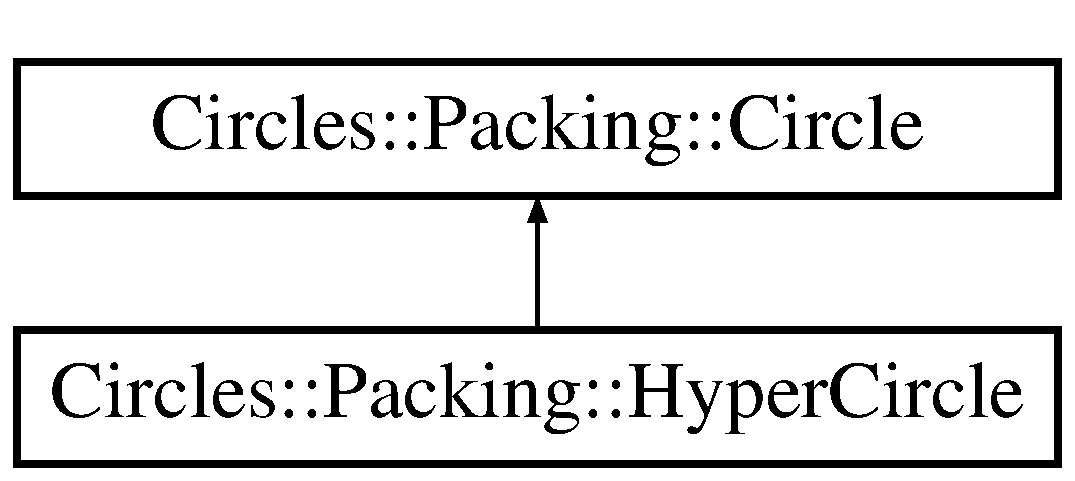
\includegraphics[height=2.000000cm]{class_circles_1_1_packing_1_1_hyper_circle}
\end{center}
\end{figure}
\subsection*{Public Member Functions}
\begin{DoxyCompactItemize}
\item 
\hyperlink{class_circles_1_1_packing_1_1_hyper_circle_a72823d6e1e4bd622760a169a909503cb}{Hyper\+Circle} ()
\item 
\hyperlink{class_circles_1_1_packing_1_1_hyper_circle_a5a129ad0ef97c5b49540fef7d41af62d}{Hyper\+Circle} (const Q\+Point\+F \&\hyperlink{class_circles_1_1_packing_1_1_hyper_circle_a51297723cfb8adac038a706dabbbb1e7}{center}, qreal \hyperlink{class_circles_1_1_packing_1_1_hyper_circle_a6d841473a2de1967aea00933f31400ed}{radius}, int \hyperlink{class_circles_1_1_packing_1_1_circle_a426d2e69ceadbbf0d119fd117102a8a9}{index})
\item 
\hyperlink{class_circles_1_1_packing_1_1_hyper_circle_a7a6d5562301bd8a3c2eced964c964706}{Hyper\+Circle} (const \hyperlink{class_circles_1_1_packing_1_1_hyper_circle}{Hyper\+Circle} \&other)
\item 
\hyperlink{class_circles_1_1_packing_1_1_hyper_circle}{Hyper\+Circle} \& \hyperlink{class_circles_1_1_packing_1_1_hyper_circle_a3c819c695e95ea5f1dfa694513d1d093}{operator=} (const \hyperlink{class_circles_1_1_packing_1_1_hyper_circle}{Hyper\+Circle} \&other)
\item 
virtual Q\+Point\+F \hyperlink{class_circles_1_1_packing_1_1_hyper_circle_a51297723cfb8adac038a706dabbbb1e7}{center} () const  override
\item 
virtual qreal \hyperlink{class_circles_1_1_packing_1_1_hyper_circle_a6d841473a2de1967aea00933f31400ed}{radius} () const  override
\item 
virtual Q\+Point\+F \hyperlink{class_circles_1_1_packing_1_1_hyper_circle_a4a00caa714bc479d2b7d777c7cf41b19}{proj\+Center} () const  override
\item 
virtual qreal \hyperlink{class_circles_1_1_packing_1_1_hyper_circle_aee965a2f67ebf52e9cf88b2eb6f53b9f}{proj\+Radius} () const  override
\item 
virtual void \hyperlink{class_circles_1_1_packing_1_1_hyper_circle_a615257ea4d789aae5641fafca8c49047}{set\+Radius} (qreal r) override
\item 
virtual bool \hyperlink{class_circles_1_1_packing_1_1_hyper_circle_a5c4e09db77fee96d649d3faba1ee0a76}{set\+Center} (Q\+Point\+F c) override
\end{DoxyCompactItemize}
\subsection*{Friends}
\begin{DoxyCompactItemize}
\item 
bool \hyperlink{class_circles_1_1_packing_1_1_hyper_circle_ab72fdf6d06653137ab83406cb05e8f61}{operator==} (const \hyperlink{class_circles_1_1_packing_1_1_hyper_circle}{Hyper\+Circle} \&lhs, const \hyperlink{class_circles_1_1_packing_1_1_hyper_circle}{Hyper\+Circle} \&rhs)
\end{DoxyCompactItemize}
\subsection*{Additional Inherited Members}


\subsection{Detailed Description}
A circle in the hyperbolic poincare disc. 

\subsection{Constructor \& Destructor Documentation}
\hypertarget{class_circles_1_1_packing_1_1_hyper_circle_a72823d6e1e4bd622760a169a909503cb}{}\index{Circles\+::\+Packing\+::\+Hyper\+Circle@{Circles\+::\+Packing\+::\+Hyper\+Circle}!Hyper\+Circle@{Hyper\+Circle}}
\index{Hyper\+Circle@{Hyper\+Circle}!Circles\+::\+Packing\+::\+Hyper\+Circle@{Circles\+::\+Packing\+::\+Hyper\+Circle}}
\subsubsection[{Hyper\+Circle()}]{\setlength{\rightskip}{0pt plus 5cm}Circles\+::\+Packing\+::\+Hyper\+Circle\+::\+Hyper\+Circle (
\begin{DoxyParamCaption}
{}
\end{DoxyParamCaption}
)}\label{class_circles_1_1_packing_1_1_hyper_circle_a72823d6e1e4bd622760a169a909503cb}
Construct an empty euclidean circle, centered at (0, 0) with radius 1.\+0, and index -\/1. \hypertarget{class_circles_1_1_packing_1_1_hyper_circle_a5a129ad0ef97c5b49540fef7d41af62d}{}\index{Circles\+::\+Packing\+::\+Hyper\+Circle@{Circles\+::\+Packing\+::\+Hyper\+Circle}!Hyper\+Circle@{Hyper\+Circle}}
\index{Hyper\+Circle@{Hyper\+Circle}!Circles\+::\+Packing\+::\+Hyper\+Circle@{Circles\+::\+Packing\+::\+Hyper\+Circle}}
\subsubsection[{Hyper\+Circle(const Q\+Point\+F \&center, qreal radius, int index)}]{\setlength{\rightskip}{0pt plus 5cm}Circles\+::\+Packing\+::\+Hyper\+Circle\+::\+Hyper\+Circle (
\begin{DoxyParamCaption}
\item[{const Q\+Point\+F \&}]{center, }
\item[{qreal}]{radius, }
\item[{int}]{index}
\end{DoxyParamCaption}
)}\label{class_circles_1_1_packing_1_1_hyper_circle_a5a129ad0ef97c5b49540fef7d41af62d}
Construct a Hyperbolic circle with a given center , radius, and index. 
\begin{DoxyParams}{Parameters}
{\em center} & Center point of the circle, in hyperbolic disc space. \\
\hline
{\em radius} & Hyperbolic Radius of the circle. \\
\hline
{\em index} & Index of corresponding node in the underlying graph. \\
\hline
\end{DoxyParams}
\hypertarget{class_circles_1_1_packing_1_1_hyper_circle_a7a6d5562301bd8a3c2eced964c964706}{}\index{Circles\+::\+Packing\+::\+Hyper\+Circle@{Circles\+::\+Packing\+::\+Hyper\+Circle}!Hyper\+Circle@{Hyper\+Circle}}
\index{Hyper\+Circle@{Hyper\+Circle}!Circles\+::\+Packing\+::\+Hyper\+Circle@{Circles\+::\+Packing\+::\+Hyper\+Circle}}
\subsubsection[{Hyper\+Circle(const Hyper\+Circle \&other)}]{\setlength{\rightskip}{0pt plus 5cm}Circles\+::\+Packing\+::\+Hyper\+Circle\+::\+Hyper\+Circle (
\begin{DoxyParamCaption}
\item[{const {\bf Hyper\+Circle} \&}]{other}
\end{DoxyParamCaption}
)}\label{class_circles_1_1_packing_1_1_hyper_circle_a7a6d5562301bd8a3c2eced964c964706}


\subsection{Member Function Documentation}
\hypertarget{class_circles_1_1_packing_1_1_hyper_circle_a51297723cfb8adac038a706dabbbb1e7}{}\index{Circles\+::\+Packing\+::\+Hyper\+Circle@{Circles\+::\+Packing\+::\+Hyper\+Circle}!center@{center}}
\index{center@{center}!Circles\+::\+Packing\+::\+Hyper\+Circle@{Circles\+::\+Packing\+::\+Hyper\+Circle}}
\subsubsection[{center() const  override}]{\setlength{\rightskip}{0pt plus 5cm}Q\+Point\+F Circles\+::\+Packing\+::\+Hyper\+Circle\+::center (
\begin{DoxyParamCaption}
{}
\end{DoxyParamCaption}
) const\hspace{0.3cm}{\ttfamily [override]}, {\ttfamily [virtual]}}\label{class_circles_1_1_packing_1_1_hyper_circle_a51297723cfb8adac038a706dabbbb1e7}
The center of the circle in it\textquotesingle{}s local space. \begin{DoxyReturn}{Returns}
The point of the center of the circle in local coordinates. 
\end{DoxyReturn}


Implements \hyperlink{class_circles_1_1_packing_1_1_circle_a2241ee34969d0c0266948cf1f23fa23a}{Circles\+::\+Packing\+::\+Circle}.

\hypertarget{class_circles_1_1_packing_1_1_hyper_circle_a3c819c695e95ea5f1dfa694513d1d093}{}\index{Circles\+::\+Packing\+::\+Hyper\+Circle@{Circles\+::\+Packing\+::\+Hyper\+Circle}!operator=@{operator=}}
\index{operator=@{operator=}!Circles\+::\+Packing\+::\+Hyper\+Circle@{Circles\+::\+Packing\+::\+Hyper\+Circle}}
\subsubsection[{operator=(const Hyper\+Circle \&other)}]{\setlength{\rightskip}{0pt plus 5cm}{\bf Hyper\+Circle} \& Circles\+::\+Packing\+::\+Hyper\+Circle\+::operator= (
\begin{DoxyParamCaption}
\item[{const {\bf Hyper\+Circle} \&}]{other}
\end{DoxyParamCaption}
)}\label{class_circles_1_1_packing_1_1_hyper_circle_a3c819c695e95ea5f1dfa694513d1d093}
\hypertarget{class_circles_1_1_packing_1_1_hyper_circle_a4a00caa714bc479d2b7d777c7cf41b19}{}\index{Circles\+::\+Packing\+::\+Hyper\+Circle@{Circles\+::\+Packing\+::\+Hyper\+Circle}!proj\+Center@{proj\+Center}}
\index{proj\+Center@{proj\+Center}!Circles\+::\+Packing\+::\+Hyper\+Circle@{Circles\+::\+Packing\+::\+Hyper\+Circle}}
\subsubsection[{proj\+Center() const  override}]{\setlength{\rightskip}{0pt plus 5cm}Q\+Point\+F Circles\+::\+Packing\+::\+Hyper\+Circle\+::proj\+Center (
\begin{DoxyParamCaption}
{}
\end{DoxyParamCaption}
) const\hspace{0.3cm}{\ttfamily [override]}, {\ttfamily [virtual]}}\label{class_circles_1_1_packing_1_1_hyper_circle_a4a00caa714bc479d2b7d777c7cf41b19}
The center of the circle when projected into euclidean space (ie as it is on the monitor). For circles that exist in Euclidean space, this will be equal to its \hyperlink{class_circles_1_1_packing_1_1_hyper_circle_a51297723cfb8adac038a706dabbbb1e7}{center()} \begin{DoxyReturn}{Returns}
the projected center of the circle. 
\end{DoxyReturn}


Implements \hyperlink{class_circles_1_1_packing_1_1_circle_a8f410a32d3d9421231512f86fb0d564e}{Circles\+::\+Packing\+::\+Circle}.

\hypertarget{class_circles_1_1_packing_1_1_hyper_circle_aee965a2f67ebf52e9cf88b2eb6f53b9f}{}\index{Circles\+::\+Packing\+::\+Hyper\+Circle@{Circles\+::\+Packing\+::\+Hyper\+Circle}!proj\+Radius@{proj\+Radius}}
\index{proj\+Radius@{proj\+Radius}!Circles\+::\+Packing\+::\+Hyper\+Circle@{Circles\+::\+Packing\+::\+Hyper\+Circle}}
\subsubsection[{proj\+Radius() const  override}]{\setlength{\rightskip}{0pt plus 5cm}qreal Circles\+::\+Packing\+::\+Hyper\+Circle\+::proj\+Radius (
\begin{DoxyParamCaption}
{}
\end{DoxyParamCaption}
) const\hspace{0.3cm}{\ttfamily [override]}, {\ttfamily [virtual]}}\label{class_circles_1_1_packing_1_1_hyper_circle_aee965a2f67ebf52e9cf88b2eb6f53b9f}
The radius of the circle when projected into euclidean space (ie as it is on the monitor). For circles that exist in Euclidean space, this will be equal to its \hyperlink{class_circles_1_1_packing_1_1_hyper_circle_a6d841473a2de1967aea00933f31400ed}{radius()}. \begin{DoxyReturn}{Returns}
the projected radius of the circle. 
\end{DoxyReturn}


Implements \hyperlink{class_circles_1_1_packing_1_1_circle_a70b927c4a58d1fe7c7576f351ce45784}{Circles\+::\+Packing\+::\+Circle}.

\hypertarget{class_circles_1_1_packing_1_1_hyper_circle_a6d841473a2de1967aea00933f31400ed}{}\index{Circles\+::\+Packing\+::\+Hyper\+Circle@{Circles\+::\+Packing\+::\+Hyper\+Circle}!radius@{radius}}
\index{radius@{radius}!Circles\+::\+Packing\+::\+Hyper\+Circle@{Circles\+::\+Packing\+::\+Hyper\+Circle}}
\subsubsection[{radius() const  override}]{\setlength{\rightskip}{0pt plus 5cm}qreal Circles\+::\+Packing\+::\+Hyper\+Circle\+::radius (
\begin{DoxyParamCaption}
{}
\end{DoxyParamCaption}
) const\hspace{0.3cm}{\ttfamily [override]}, {\ttfamily [virtual]}}\label{class_circles_1_1_packing_1_1_hyper_circle_a6d841473a2de1967aea00933f31400ed}
The radius of the circle in its local space. \begin{DoxyReturn}{Returns}
radius of the circle in its local space. 
\end{DoxyReturn}


Implements \hyperlink{class_circles_1_1_packing_1_1_circle_a3e34226854bcbcbd9e462e1e4fe54005}{Circles\+::\+Packing\+::\+Circle}.

\hypertarget{class_circles_1_1_packing_1_1_hyper_circle_a5c4e09db77fee96d649d3faba1ee0a76}{}\index{Circles\+::\+Packing\+::\+Hyper\+Circle@{Circles\+::\+Packing\+::\+Hyper\+Circle}!set\+Center@{set\+Center}}
\index{set\+Center@{set\+Center}!Circles\+::\+Packing\+::\+Hyper\+Circle@{Circles\+::\+Packing\+::\+Hyper\+Circle}}
\subsubsection[{set\+Center(\+Q\+Point\+F c) override}]{\setlength{\rightskip}{0pt plus 5cm}bool Circles\+::\+Packing\+::\+Hyper\+Circle\+::set\+Center (
\begin{DoxyParamCaption}
\item[{Q\+Point\+F}]{c}
\end{DoxyParamCaption}
)\hspace{0.3cm}{\ttfamily [override]}, {\ttfamily [virtual]}}\label{class_circles_1_1_packing_1_1_hyper_circle_a5c4e09db77fee96d649d3faba1ee0a76}
Attempt to set the center of the circle. 
\begin{DoxyParams}{Parameters}
{\em c} & the center to set \\
\hline
\end{DoxyParams}
\begin{DoxyReturn}{Returns}
True if the center was set correctly. False otherwise. 
\end{DoxyReturn}


Implements \hyperlink{class_circles_1_1_packing_1_1_circle_a335f807f081d7f97fdea6e6d84cbc46e}{Circles\+::\+Packing\+::\+Circle}.

\hypertarget{class_circles_1_1_packing_1_1_hyper_circle_a615257ea4d789aae5641fafca8c49047}{}\index{Circles\+::\+Packing\+::\+Hyper\+Circle@{Circles\+::\+Packing\+::\+Hyper\+Circle}!set\+Radius@{set\+Radius}}
\index{set\+Radius@{set\+Radius}!Circles\+::\+Packing\+::\+Hyper\+Circle@{Circles\+::\+Packing\+::\+Hyper\+Circle}}
\subsubsection[{set\+Radius(qreal r) override}]{\setlength{\rightskip}{0pt plus 5cm}void Circles\+::\+Packing\+::\+Hyper\+Circle\+::set\+Radius (
\begin{DoxyParamCaption}
\item[{qreal}]{r}
\end{DoxyParamCaption}
)\hspace{0.3cm}{\ttfamily [override]}, {\ttfamily [virtual]}}\label{class_circles_1_1_packing_1_1_hyper_circle_a615257ea4d789aae5641fafca8c49047}
Set the radius of the circle to the specified value. 
\begin{DoxyParams}{Parameters}
{\em r} & The new radius of the circle. (in local space) \\
\hline
\end{DoxyParams}


Implements \hyperlink{class_circles_1_1_packing_1_1_circle_a7ed2112528b874aa2cb58854eb844b7c}{Circles\+::\+Packing\+::\+Circle}.



\subsection{Friends And Related Function Documentation}
\hypertarget{class_circles_1_1_packing_1_1_hyper_circle_ab72fdf6d06653137ab83406cb05e8f61}{}\index{Circles\+::\+Packing\+::\+Hyper\+Circle@{Circles\+::\+Packing\+::\+Hyper\+Circle}!operator==@{operator==}}
\index{operator==@{operator==}!Circles\+::\+Packing\+::\+Hyper\+Circle@{Circles\+::\+Packing\+::\+Hyper\+Circle}}
\subsubsection[{operator==}]{\setlength{\rightskip}{0pt plus 5cm}bool operator== (
\begin{DoxyParamCaption}
\item[{const {\bf Hyper\+Circle} \&}]{lhs, }
\item[{const {\bf Hyper\+Circle} \&}]{rhs}
\end{DoxyParamCaption}
)\hspace{0.3cm}{\ttfamily [friend]}}\label{class_circles_1_1_packing_1_1_hyper_circle_ab72fdf6d06653137ab83406cb05e8f61}


The documentation for this class was generated from the following files\+:\begin{DoxyCompactItemize}
\item 
packing/\hyperlink{_hyper_circle_8hpp}{Hyper\+Circle.\+hpp}\item 
packing/\hyperlink{_hyper_circle_8cpp}{Hyper\+Circle.\+cpp}\end{DoxyCompactItemize}

\hypertarget{class_main_window}{}\section{Main\+Window Class Reference}
\label{class_main_window}\index{Main\+Window@{Main\+Window}}


{\ttfamily \#include $<$Main\+Window.\+hpp$>$}

Inheritance diagram for Main\+Window\+:\begin{figure}[H]
\begin{center}
\leavevmode
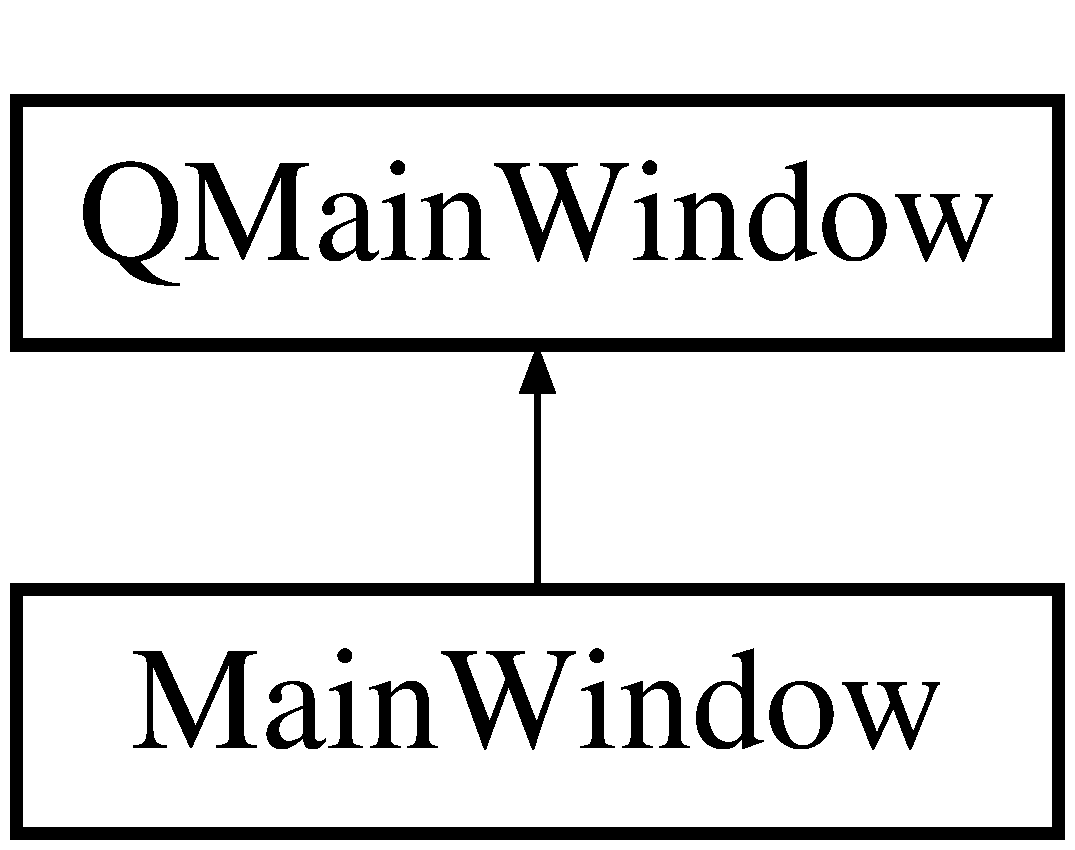
\includegraphics[height=2.000000cm]{class_main_window}
\end{center}
\end{figure}
\subsection*{Public Member Functions}
\begin{DoxyCompactItemize}
\item 
\hyperlink{class_main_window_a8b244be8b7b7db1b08de2a2acb9409db}{Main\+Window} (Q\+Widget $\ast$parent=0)
\item 
\hyperlink{class_main_window_ae98d00a93bc118200eeef9f9bba1dba7}{$\sim$\+Main\+Window} ()
\end{DoxyCompactItemize}


\subsection{Constructor \& Destructor Documentation}
\hypertarget{class_main_window_a8b244be8b7b7db1b08de2a2acb9409db}{}\index{Main\+Window@{Main\+Window}!Main\+Window@{Main\+Window}}
\index{Main\+Window@{Main\+Window}!Main\+Window@{Main\+Window}}
\subsubsection[{Main\+Window(\+Q\+Widget $\ast$parent=0)}]{\setlength{\rightskip}{0pt plus 5cm}Main\+Window\+::\+Main\+Window (
\begin{DoxyParamCaption}
\item[{Q\+Widget $\ast$}]{parent = {\ttfamily 0}}
\end{DoxyParamCaption}
)\hspace{0.3cm}{\ttfamily [explicit]}}\label{class_main_window_a8b244be8b7b7db1b08de2a2acb9409db}
\hypertarget{class_main_window_ae98d00a93bc118200eeef9f9bba1dba7}{}\index{Main\+Window@{Main\+Window}!````~Main\+Window@{$\sim$\+Main\+Window}}
\index{````~Main\+Window@{$\sim$\+Main\+Window}!Main\+Window@{Main\+Window}}
\subsubsection[{$\sim$\+Main\+Window()}]{\setlength{\rightskip}{0pt plus 5cm}Main\+Window\+::$\sim$\+Main\+Window (
\begin{DoxyParamCaption}
{}
\end{DoxyParamCaption}
)}\label{class_main_window_ae98d00a93bc118200eeef9f9bba1dba7}


The documentation for this class was generated from the following files\+:\begin{DoxyCompactItemize}
\item 
ui/\hyperlink{_main_window_8hpp}{Main\+Window.\+hpp}\item 
ui/\hyperlink{_main_window_8cpp}{Main\+Window.\+cpp}\end{DoxyCompactItemize}

\hypertarget{class_node}{}\section{Node Class Reference}
\label{class_node}\index{Node@{Node}}


The \hyperlink{class_node}{Node} class represents the metadata of a circle in a circle packing.  




{\ttfamily \#include $<$Node.\+hpp$>$}

\subsection*{Public Member Functions}
\begin{DoxyCompactItemize}
\item 
\hyperlink{class_node_a1cb59fd72bfc69d4b741e091652a4365}{Node} (const \hyperlink{class_node}{Node} $\ast$n)
\item 
\hyperlink{class_node_a7f1af54cb91467d9717155c8a2ac0fde}{Node} (int \hyperlink{class_node_a59a543130a10c95f1e8642cf8c5645e8}{id})
\item 
\hyperlink{class_node_a4989e0d6f4483993bef734eaaeabb817}{Node} (int \hyperlink{class_node_a59a543130a10c95f1e8642cf8c5645e8}{id}, const Q\+Point\+F \&\hyperlink{class_node_af0201de36fd117a362e5f52fd6d75cde}{position}, qreal \hyperlink{class_node_abc1468f478d90c8d205b5753eacb1f3b}{radius}=0)
\item 
\hyperlink{class_node_aa0840c3cb5c7159be6d992adecd2097c}{$\sim$\+Node} ()
\item 
int \hyperlink{class_node_a3c7b8ccf4dab44216b997c5f63f11d9f}{get\+Id} ()
\item 
void \hyperlink{class_node_aa2755c83e214f119c0033ef1286cdb26}{set\+Id} (int value)
\item 
qreal \hyperlink{class_node_ad178553d97281f8dc87173323ef1254e}{get\+Radius} ()
\item 
void \hyperlink{class_node_ac460b65aa4b024fa1ae613f36e3d3f87}{set\+Radius} (const qreal value)
\item 
Q\+Color \hyperlink{class_node_a6c675f2c58d53abc9921871919a45f33}{get\+Color} ()
\item 
void \hyperlink{class_node_a44f165302fa884ac057ed6acc256d6e1}{set\+Color} (const Q\+Color \&value)
\item 
void \hyperlink{class_node_a1759916d01600ffcd414fd9035669ff0}{add\+Neibhour} (\hyperlink{class_node}{Node} $\ast$node)
\item 
void \hyperlink{class_node_a18f47997870bbf1d56bbe9814e566425}{del\+Neibhour} (\hyperlink{class_node}{Node} $\ast$node)
\item 
void \hyperlink{class_node_a2e7ae32f9ae0addc356281d9593ef5ba}{purge\+Neibhours} ()
\item 
bool \hyperlink{class_node_aa0e6fa73b1c95c5405dee1e10ff1881f}{is\+Neibhour} (\hyperlink{class_node}{Node} $\ast$node)
\item 
void \hyperlink{class_node_ac0f32d921f5849c5edce7c76e245b516}{sort\+Neibhours} ()
\item 
Q\+List$<$ \hyperlink{class_node}{Node} $\ast$ $>$ \hyperlink{class_node_aef487f3aed9670249dcd2b07406d48dd}{get\+Neibhours} ()
\item 
int \hyperlink{class_node_a5a05aa880682f3021bdbb5d7cad70641}{get\+Neibhour\+Count} ()
\item 
void \hyperlink{class_node_a4e3af9f1b628ef5458e6097a5624b144}{set\+Position} (const Q\+Point\+F \&\hyperlink{class_node_af0201de36fd117a362e5f52fd6d75cde}{position})
\item 
Q\+Point\+F \hyperlink{class_node_aa7e8b720e25e39a0719d8ba03bf69cf4}{get\+Position} ()
\item 
bool \hyperlink{class_node_a0ea70d198511ebbeb027fa8d632c974d}{has\+Position} ()
\item 
void \hyperlink{class_node_a2b99358139b61f8ff4b0c85055bf1f22}{del\+Position} ()
\item 
bool \hyperlink{class_node_ada64122ca79cadfc50518871e64fc208}{has\+Full\+Flower} ()
\end{DoxyCompactItemize}
\subsection*{Static Public Member Functions}
\begin{DoxyCompactItemize}
\item 
static Q\+List$<$ \hyperlink{class_node}{Node} $\ast$ $>$ \hyperlink{class_node_a139278bba2f9090857f01d3339a87753}{generate\+Hex\+Array} (const Q\+Rect\+F \&area, qreal \hyperlink{class_node_abc1468f478d90c8d205b5753eacb1f3b}{radius})
\item 
static Q\+List$<$ \hyperlink{class_node}{Node} $\ast$ $>$ \hyperlink{class_node_ac35036093a7bda3b0d70224418c5b1ef}{generate\+Hex\+Array} (const Q\+Point\+F \&startpos, int w, int h, qreal \hyperlink{class_node_abc1468f478d90c8d205b5753eacb1f3b}{radius})
\end{DoxyCompactItemize}
\subsection*{Protected Attributes}
\begin{DoxyCompactItemize}
\item 
int \hyperlink{class_node_a59a543130a10c95f1e8642cf8c5645e8}{id}
\item 
Q\+Point\+F \hyperlink{class_node_af0201de36fd117a362e5f52fd6d75cde}{position}
\item 
qreal \hyperlink{class_node_abc1468f478d90c8d205b5753eacb1f3b}{radius}
\item 
Q\+List$<$ \hyperlink{class_node}{Node} $\ast$ $>$ \hyperlink{class_node_a3521ee4be71939435cd4f043f0295d45}{neibhours}
\item 
Q\+Color \hyperlink{class_node_a90575cbf03f1a5f4655fa7ed15354d51}{color}
\item 
bool \hyperlink{class_node_a62e8fc19070ec04df18488c16933cb1a}{b\+Has\+Position} =false
\item 
bool \hyperlink{class_node_a39c984cfd740ca7968dc6a62c2b87570}{sorted\+Neibhours} =false
\end{DoxyCompactItemize}


\subsection{Detailed Description}
The \hyperlink{class_node}{Node} class represents the metadata of a circle in a circle packing. 

\subsection{Constructor \& Destructor Documentation}
\hypertarget{class_node_a1cb59fd72bfc69d4b741e091652a4365}{}\index{Node@{Node}!Node@{Node}}
\index{Node@{Node}!Node@{Node}}
\subsubsection[{Node(const Node $\ast$n)}]{\setlength{\rightskip}{0pt plus 5cm}Node\+::\+Node (
\begin{DoxyParamCaption}
\item[{const {\bf Node} $\ast$}]{n}
\end{DoxyParamCaption}
)}\label{class_node_a1cb59fd72bfc69d4b741e091652a4365}
Copy constructor. Note that neibhour relationships are not copied. 
\begin{DoxyParams}{Parameters}
{\em n} & \hyperlink{class_node}{Node} to copy \\
\hline
\end{DoxyParams}
\hypertarget{class_node_a7f1af54cb91467d9717155c8a2ac0fde}{}\index{Node@{Node}!Node@{Node}}
\index{Node@{Node}!Node@{Node}}
\subsubsection[{Node(int id)}]{\setlength{\rightskip}{0pt plus 5cm}Node\+::\+Node (
\begin{DoxyParamCaption}
\item[{int}]{id}
\end{DoxyParamCaption}
)}\label{class_node_a7f1af54cb91467d9717155c8a2ac0fde}
Construct a \hyperlink{class_node}{Node} without position or radius. 
\begin{DoxyParams}{Parameters}
{\em id} & unique id of the node \\
\hline
\end{DoxyParams}
\hypertarget{class_node_a4989e0d6f4483993bef734eaaeabb817}{}\index{Node@{Node}!Node@{Node}}
\index{Node@{Node}!Node@{Node}}
\subsubsection[{Node(int id, const Q\+Point\+F \&position, qreal radius=0)}]{\setlength{\rightskip}{0pt plus 5cm}Node\+::\+Node (
\begin{DoxyParamCaption}
\item[{int}]{id, }
\item[{const Q\+Point\+F \&}]{position, }
\item[{qreal}]{radius = {\ttfamily 0}}
\end{DoxyParamCaption}
)}\label{class_node_a4989e0d6f4483993bef734eaaeabb817}
Construct a node with a given position and radius. 
\begin{DoxyParams}{Parameters}
{\em id} & Unique id of the node \\
\hline
{\em position} & Position of the node \\
\hline
{\em radius} & radius of the node \\
\hline
\end{DoxyParams}
\hypertarget{class_node_aa0840c3cb5c7159be6d992adecd2097c}{}\index{Node@{Node}!````~Node@{$\sim$\+Node}}
\index{````~Node@{$\sim$\+Node}!Node@{Node}}
\subsubsection[{$\sim$\+Node()}]{\setlength{\rightskip}{0pt plus 5cm}Node\+::$\sim$\+Node (
\begin{DoxyParamCaption}
{}
\end{DoxyParamCaption}
)}\label{class_node_aa0840c3cb5c7159be6d992adecd2097c}


\subsection{Member Function Documentation}
\hypertarget{class_node_a1759916d01600ffcd414fd9035669ff0}{}\index{Node@{Node}!add\+Neibhour@{add\+Neibhour}}
\index{add\+Neibhour@{add\+Neibhour}!Node@{Node}}
\subsubsection[{add\+Neibhour(\+Node $\ast$node)}]{\setlength{\rightskip}{0pt plus 5cm}void Node\+::add\+Neibhour (
\begin{DoxyParamCaption}
\item[{{\bf Node} $\ast$}]{node}
\end{DoxyParamCaption}
)}\label{class_node_a1759916d01600ffcd414fd9035669ff0}
\hypertarget{class_node_a18f47997870bbf1d56bbe9814e566425}{}\index{Node@{Node}!del\+Neibhour@{del\+Neibhour}}
\index{del\+Neibhour@{del\+Neibhour}!Node@{Node}}
\subsubsection[{del\+Neibhour(\+Node $\ast$node)}]{\setlength{\rightskip}{0pt plus 5cm}void Node\+::del\+Neibhour (
\begin{DoxyParamCaption}
\item[{{\bf Node} $\ast$}]{node}
\end{DoxyParamCaption}
)}\label{class_node_a18f47997870bbf1d56bbe9814e566425}
\hypertarget{class_node_a2b99358139b61f8ff4b0c85055bf1f22}{}\index{Node@{Node}!del\+Position@{del\+Position}}
\index{del\+Position@{del\+Position}!Node@{Node}}
\subsubsection[{del\+Position()}]{\setlength{\rightskip}{0pt plus 5cm}void Node\+::del\+Position (
\begin{DoxyParamCaption}
{}
\end{DoxyParamCaption}
)}\label{class_node_a2b99358139b61f8ff4b0c85055bf1f22}
\hypertarget{class_node_a139278bba2f9090857f01d3339a87753}{}\index{Node@{Node}!generate\+Hex\+Array@{generate\+Hex\+Array}}
\index{generate\+Hex\+Array@{generate\+Hex\+Array}!Node@{Node}}
\subsubsection[{generate\+Hex\+Array(const Q\+Rect\+F \&area, qreal radius)}]{\setlength{\rightskip}{0pt plus 5cm}Q\+List$<$ {\bf Node} $\ast$ $>$ Node\+::generate\+Hex\+Array (
\begin{DoxyParamCaption}
\item[{const Q\+Rect\+F \&}]{area, }
\item[{qreal}]{radius}
\end{DoxyParamCaption}
)\hspace{0.3cm}{\ttfamily [static]}}\label{class_node_a139278bba2f9090857f01d3339a87753}
Generates a hex tiling of circles with specified radius such that circles are guaranteed to cover at least the specified area 
\begin{DoxyParams}{Parameters}
{\em area} & the area to cover \\
\hline
{\em radius} & radius of the circles \\
\hline
\end{DoxyParams}
\begin{DoxyReturn}{Returns}
list of nodes representing the circles created. 
\end{DoxyReturn}
\hypertarget{class_node_ac35036093a7bda3b0d70224418c5b1ef}{}\index{Node@{Node}!generate\+Hex\+Array@{generate\+Hex\+Array}}
\index{generate\+Hex\+Array@{generate\+Hex\+Array}!Node@{Node}}
\subsubsection[{generate\+Hex\+Array(const Q\+Point\+F \&startpos, int w, int h, qreal radius)}]{\setlength{\rightskip}{0pt plus 5cm}Q\+List$<$ {\bf Node} $\ast$ $>$ Node\+::generate\+Hex\+Array (
\begin{DoxyParamCaption}
\item[{const Q\+Point\+F \&}]{startpos, }
\item[{int}]{w, }
\item[{int}]{h, }
\item[{qreal}]{radius}
\end{DoxyParamCaption}
)\hspace{0.3cm}{\ttfamily [static]}}\label{class_node_ac35036093a7bda3b0d70224418c5b1ef}

\begin{DoxyParams}{Parameters}
{\em startpos} & the location of the top-\/left circle \\
\hline
{\em w} & width, in circles, of the circle array \\
\hline
{\em h} & height, in circles, of the circle array. Should be odd. \\
\hline
{\em radius} & the radius of each circle. \\
\hline
\end{DoxyParams}
\begin{DoxyReturn}{Returns}
list of nodes representing the circles created. 
\end{DoxyReturn}
\hypertarget{class_node_a6c675f2c58d53abc9921871919a45f33}{}\index{Node@{Node}!get\+Color@{get\+Color}}
\index{get\+Color@{get\+Color}!Node@{Node}}
\subsubsection[{get\+Color()}]{\setlength{\rightskip}{0pt plus 5cm}Q\+Color Node\+::get\+Color (
\begin{DoxyParamCaption}
{}
\end{DoxyParamCaption}
)}\label{class_node_a6c675f2c58d53abc9921871919a45f33}
\hypertarget{class_node_a3c7b8ccf4dab44216b997c5f63f11d9f}{}\index{Node@{Node}!get\+Id@{get\+Id}}
\index{get\+Id@{get\+Id}!Node@{Node}}
\subsubsection[{get\+Id()}]{\setlength{\rightskip}{0pt plus 5cm}int Node\+::get\+Id (
\begin{DoxyParamCaption}
{}
\end{DoxyParamCaption}
)}\label{class_node_a3c7b8ccf4dab44216b997c5f63f11d9f}
\hypertarget{class_node_a5a05aa880682f3021bdbb5d7cad70641}{}\index{Node@{Node}!get\+Neibhour\+Count@{get\+Neibhour\+Count}}
\index{get\+Neibhour\+Count@{get\+Neibhour\+Count}!Node@{Node}}
\subsubsection[{get\+Neibhour\+Count()}]{\setlength{\rightskip}{0pt plus 5cm}int Node\+::get\+Neibhour\+Count (
\begin{DoxyParamCaption}
{}
\end{DoxyParamCaption}
)}\label{class_node_a5a05aa880682f3021bdbb5d7cad70641}
\hypertarget{class_node_aef487f3aed9670249dcd2b07406d48dd}{}\index{Node@{Node}!get\+Neibhours@{get\+Neibhours}}
\index{get\+Neibhours@{get\+Neibhours}!Node@{Node}}
\subsubsection[{get\+Neibhours()}]{\setlength{\rightskip}{0pt plus 5cm}Q\+List$<$ {\bf Node} $\ast$ $>$ Node\+::get\+Neibhours (
\begin{DoxyParamCaption}
{}
\end{DoxyParamCaption}
)}\label{class_node_aef487f3aed9670249dcd2b07406d48dd}
\hypertarget{class_node_aa7e8b720e25e39a0719d8ba03bf69cf4}{}\index{Node@{Node}!get\+Position@{get\+Position}}
\index{get\+Position@{get\+Position}!Node@{Node}}
\subsubsection[{get\+Position()}]{\setlength{\rightskip}{0pt plus 5cm}Q\+Point\+F Node\+::get\+Position (
\begin{DoxyParamCaption}
{}
\end{DoxyParamCaption}
)}\label{class_node_aa7e8b720e25e39a0719d8ba03bf69cf4}
\hypertarget{class_node_ad178553d97281f8dc87173323ef1254e}{}\index{Node@{Node}!get\+Radius@{get\+Radius}}
\index{get\+Radius@{get\+Radius}!Node@{Node}}
\subsubsection[{get\+Radius()}]{\setlength{\rightskip}{0pt plus 5cm}qreal Node\+::get\+Radius (
\begin{DoxyParamCaption}
{}
\end{DoxyParamCaption}
)}\label{class_node_ad178553d97281f8dc87173323ef1254e}
\hypertarget{class_node_ada64122ca79cadfc50518871e64fc208}{}\index{Node@{Node}!has\+Full\+Flower@{has\+Full\+Flower}}
\index{has\+Full\+Flower@{has\+Full\+Flower}!Node@{Node}}
\subsubsection[{has\+Full\+Flower()}]{\setlength{\rightskip}{0pt plus 5cm}bool Node\+::has\+Full\+Flower (
\begin{DoxyParamCaption}
{}
\end{DoxyParamCaption}
)}\label{class_node_ada64122ca79cadfc50518871e64fc208}
\hypertarget{class_node_a0ea70d198511ebbeb027fa8d632c974d}{}\index{Node@{Node}!has\+Position@{has\+Position}}
\index{has\+Position@{has\+Position}!Node@{Node}}
\subsubsection[{has\+Position()}]{\setlength{\rightskip}{0pt plus 5cm}bool Node\+::has\+Position (
\begin{DoxyParamCaption}
{}
\end{DoxyParamCaption}
)}\label{class_node_a0ea70d198511ebbeb027fa8d632c974d}
\hypertarget{class_node_aa0e6fa73b1c95c5405dee1e10ff1881f}{}\index{Node@{Node}!is\+Neibhour@{is\+Neibhour}}
\index{is\+Neibhour@{is\+Neibhour}!Node@{Node}}
\subsubsection[{is\+Neibhour(\+Node $\ast$node)}]{\setlength{\rightskip}{0pt plus 5cm}bool Node\+::is\+Neibhour (
\begin{DoxyParamCaption}
\item[{{\bf Node} $\ast$}]{node}
\end{DoxyParamCaption}
)}\label{class_node_aa0e6fa73b1c95c5405dee1e10ff1881f}
\hypertarget{class_node_a2e7ae32f9ae0addc356281d9593ef5ba}{}\index{Node@{Node}!purge\+Neibhours@{purge\+Neibhours}}
\index{purge\+Neibhours@{purge\+Neibhours}!Node@{Node}}
\subsubsection[{purge\+Neibhours()}]{\setlength{\rightskip}{0pt plus 5cm}void Node\+::purge\+Neibhours (
\begin{DoxyParamCaption}
{}
\end{DoxyParamCaption}
)}\label{class_node_a2e7ae32f9ae0addc356281d9593ef5ba}
\hypertarget{class_node_a44f165302fa884ac057ed6acc256d6e1}{}\index{Node@{Node}!set\+Color@{set\+Color}}
\index{set\+Color@{set\+Color}!Node@{Node}}
\subsubsection[{set\+Color(const Q\+Color \&value)}]{\setlength{\rightskip}{0pt plus 5cm}void Node\+::set\+Color (
\begin{DoxyParamCaption}
\item[{const Q\+Color \&}]{value}
\end{DoxyParamCaption}
)}\label{class_node_a44f165302fa884ac057ed6acc256d6e1}
\hypertarget{class_node_aa2755c83e214f119c0033ef1286cdb26}{}\index{Node@{Node}!set\+Id@{set\+Id}}
\index{set\+Id@{set\+Id}!Node@{Node}}
\subsubsection[{set\+Id(int value)}]{\setlength{\rightskip}{0pt plus 5cm}void Node\+::set\+Id (
\begin{DoxyParamCaption}
\item[{int}]{value}
\end{DoxyParamCaption}
)}\label{class_node_aa2755c83e214f119c0033ef1286cdb26}
\hypertarget{class_node_a4e3af9f1b628ef5458e6097a5624b144}{}\index{Node@{Node}!set\+Position@{set\+Position}}
\index{set\+Position@{set\+Position}!Node@{Node}}
\subsubsection[{set\+Position(const Q\+Point\+F \&position)}]{\setlength{\rightskip}{0pt plus 5cm}void Node\+::set\+Position (
\begin{DoxyParamCaption}
\item[{const Q\+Point\+F \&}]{position}
\end{DoxyParamCaption}
)}\label{class_node_a4e3af9f1b628ef5458e6097a5624b144}
\hypertarget{class_node_ac460b65aa4b024fa1ae613f36e3d3f87}{}\index{Node@{Node}!set\+Radius@{set\+Radius}}
\index{set\+Radius@{set\+Radius}!Node@{Node}}
\subsubsection[{set\+Radius(const qreal value)}]{\setlength{\rightskip}{0pt plus 5cm}void Node\+::set\+Radius (
\begin{DoxyParamCaption}
\item[{const qreal}]{value}
\end{DoxyParamCaption}
)}\label{class_node_ac460b65aa4b024fa1ae613f36e3d3f87}
\hypertarget{class_node_ac0f32d921f5849c5edce7c76e245b516}{}\index{Node@{Node}!sort\+Neibhours@{sort\+Neibhours}}
\index{sort\+Neibhours@{sort\+Neibhours}!Node@{Node}}
\subsubsection[{sort\+Neibhours()}]{\setlength{\rightskip}{0pt plus 5cm}void Node\+::sort\+Neibhours (
\begin{DoxyParamCaption}
{}
\end{DoxyParamCaption}
)}\label{class_node_ac0f32d921f5849c5edce7c76e245b516}


\subsection{Member Data Documentation}
\hypertarget{class_node_a62e8fc19070ec04df18488c16933cb1a}{}\index{Node@{Node}!b\+Has\+Position@{b\+Has\+Position}}
\index{b\+Has\+Position@{b\+Has\+Position}!Node@{Node}}
\subsubsection[{b\+Has\+Position}]{\setlength{\rightskip}{0pt plus 5cm}bool Node\+::b\+Has\+Position =false\hspace{0.3cm}{\ttfamily [protected]}}\label{class_node_a62e8fc19070ec04df18488c16933cb1a}
\hypertarget{class_node_a90575cbf03f1a5f4655fa7ed15354d51}{}\index{Node@{Node}!color@{color}}
\index{color@{color}!Node@{Node}}
\subsubsection[{color}]{\setlength{\rightskip}{0pt plus 5cm}Q\+Color Node\+::color\hspace{0.3cm}{\ttfamily [protected]}}\label{class_node_a90575cbf03f1a5f4655fa7ed15354d51}
\hypertarget{class_node_a59a543130a10c95f1e8642cf8c5645e8}{}\index{Node@{Node}!id@{id}}
\index{id@{id}!Node@{Node}}
\subsubsection[{id}]{\setlength{\rightskip}{0pt plus 5cm}int Node\+::id\hspace{0.3cm}{\ttfamily [protected]}}\label{class_node_a59a543130a10c95f1e8642cf8c5645e8}
\hypertarget{class_node_a3521ee4be71939435cd4f043f0295d45}{}\index{Node@{Node}!neibhours@{neibhours}}
\index{neibhours@{neibhours}!Node@{Node}}
\subsubsection[{neibhours}]{\setlength{\rightskip}{0pt plus 5cm}Q\+List$<${\bf Node}$\ast$$>$ Node\+::neibhours\hspace{0.3cm}{\ttfamily [protected]}}\label{class_node_a3521ee4be71939435cd4f043f0295d45}
\hypertarget{class_node_af0201de36fd117a362e5f52fd6d75cde}{}\index{Node@{Node}!position@{position}}
\index{position@{position}!Node@{Node}}
\subsubsection[{position}]{\setlength{\rightskip}{0pt plus 5cm}Q\+Point\+F Node\+::position\hspace{0.3cm}{\ttfamily [protected]}}\label{class_node_af0201de36fd117a362e5f52fd6d75cde}
\hypertarget{class_node_abc1468f478d90c8d205b5753eacb1f3b}{}\index{Node@{Node}!radius@{radius}}
\index{radius@{radius}!Node@{Node}}
\subsubsection[{radius}]{\setlength{\rightskip}{0pt plus 5cm}qreal Node\+::radius\hspace{0.3cm}{\ttfamily [protected]}}\label{class_node_abc1468f478d90c8d205b5753eacb1f3b}
\hypertarget{class_node_a39c984cfd740ca7968dc6a62c2b87570}{}\index{Node@{Node}!sorted\+Neibhours@{sorted\+Neibhours}}
\index{sorted\+Neibhours@{sorted\+Neibhours}!Node@{Node}}
\subsubsection[{sorted\+Neibhours}]{\setlength{\rightskip}{0pt plus 5cm}bool Node\+::sorted\+Neibhours =false\hspace{0.3cm}{\ttfamily [protected]}}\label{class_node_a39c984cfd740ca7968dc6a62c2b87570}


The documentation for this class was generated from the following files\+:\begin{DoxyCompactItemize}
\item 
\hyperlink{_node_8hpp}{Node.\+hpp}\item 
\hyperlink{_node_8cpp}{Node.\+cpp}\end{DoxyCompactItemize}

\hypertarget{class_packing}{}\section{Packing Class Reference}
\label{class_packing}\index{Packing@{Packing}}


The \hyperlink{class_packing}{Packing} class is an abstract class which defines a circle packing. A circle packing may be either euclidean or hyperbolic, as found in Euclidean\+Packing and Hyperbolic\+Packing.  




{\ttfamily \#include $<$Packing.\+hpp$>$}

Inheritance diagram for Packing\+:\begin{figure}[H]
\begin{center}
\leavevmode
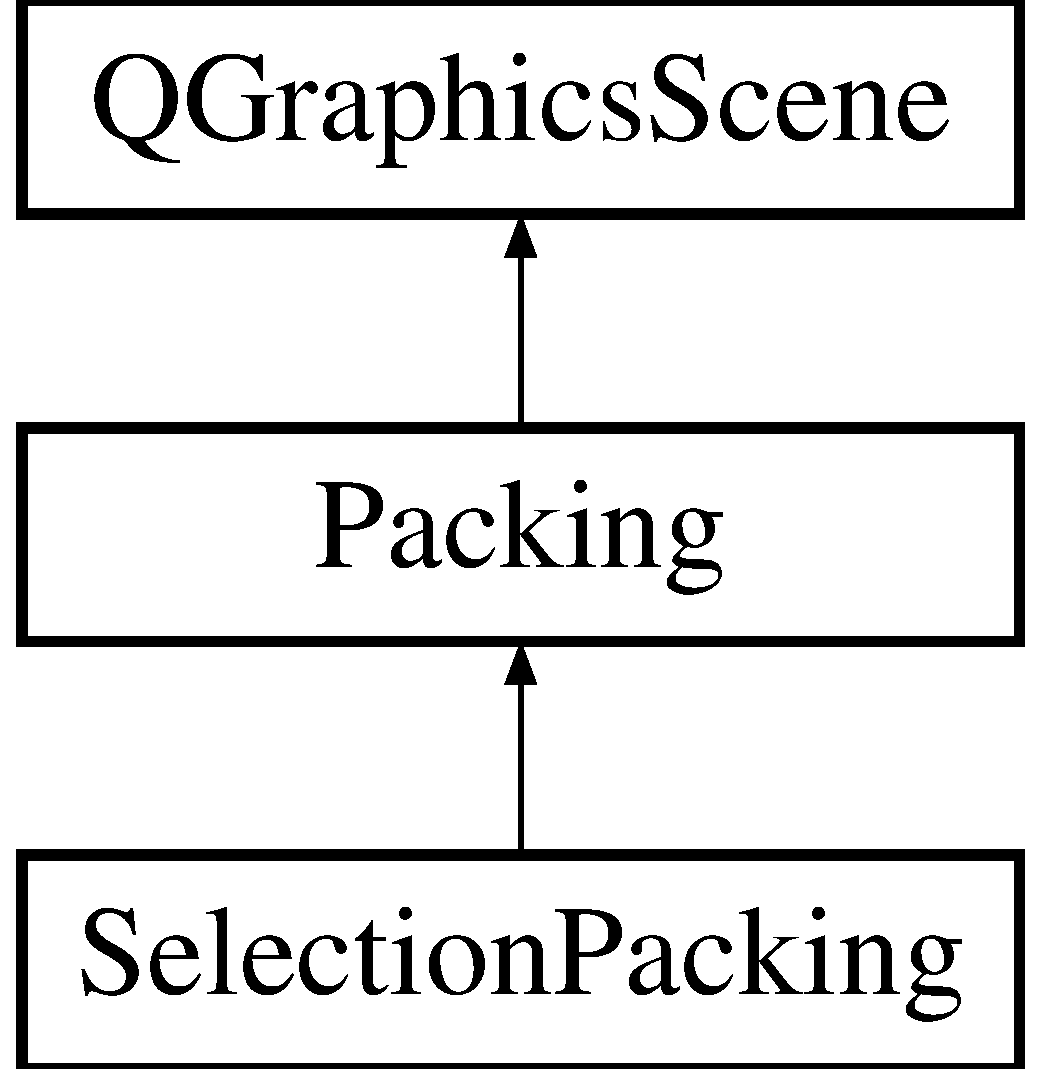
\includegraphics[height=3.000000cm]{class_packing}
\end{center}
\end{figure}
\subsection*{Public Slots}
\begin{DoxyCompactItemize}
\item 
void \hyperlink{class_packing_a3c5bdaac16b7f59c966bfa3e2572bfec}{set\+Draw\+Centers} (bool d)
\item 
void \hyperlink{class_packing_a8d95224738fdcfe7c27886c75a21a888}{set\+Draw\+Links} (bool d)
\item 
void \hyperlink{class_packing_adb39ee29cf54d899d2c7f3d924aca3e7}{set\+Draw\+Circles} (bool d)
\item 
void \hyperlink{class_packing_ae204c78072c0397bd55bb0d762258507}{set\+Draw\+Indicies} (bool d)
\item 
void \hyperlink{class_packing_a38f38eef21a2e8277a98c4d12f68f4e3}{set\+Draw\+Boundary} (bool d)
\item 
void \hyperlink{class_packing_a1a1ad296a875c5fe6463366296b389d4}{repack} (qreal epsilon, qreal outer\+Radius)
\begin{DoxyCompactList}\small\item\em Compute the radii of the circles that will result in an actual packing. \end{DoxyCompactList}\item 
void \hyperlink{class_packing_adc779649742314f9c9eaee0f43b1000a}{layout} (int center\+Circle)
\begin{DoxyCompactList}\small\item\em lay-\/out circles once radii have been computed. \end{DoxyCompactList}\end{DoxyCompactItemize}
\subsection*{Signals}
\begin{DoxyCompactItemize}
\item 
void \hyperlink{class_packing_a6c641c5342b0a9f0cdf6a5286da1faef}{new\+Node\+Selected} (\hyperlink{class_node}{Node} $\ast$n)
\end{DoxyCompactItemize}
\subsection*{Public Member Functions}
\begin{DoxyCompactItemize}
\item 
\hyperlink{class_packing_afc2e978d83701a4f45cf4c3a397d669d}{Packing} (const \hyperlink{class_packing}{Packing} $\ast$p)
\item 
\hyperlink{class_packing_ac182cdb0765b020bb5289d0980cf1fd6}{Packing} (\hyperlink{graphics_2_packing_8hpp_a331874350131c9e1039dac50b427f8b9}{Packing\+Type} \hyperlink{class_packing_a934cbe1ef81173f5e7fbabf9846d16e2}{type}=\hyperlink{graphics_2_packing_8hpp_a331874350131c9e1039dac50b427f8b9aa4066bbe6791ed6bbfe12f55a60ed152}{Packing\+Type\+::\+Euclidean\+Packing})
\begin{DoxyCompactList}\small\item\em Create a new, empty \hyperlink{class_packing}{Packing} object with specified geometry. \end{DoxyCompactList}\item 
\hyperlink{class_packing_a4091c1456760961dee4d94ed5f440ac4}{Packing} (Q\+List$<$ \hyperlink{class_node}{Node} $\ast$ $>$ \hyperlink{class_packing_afee4e76e75aea147685840e19c714d08}{nodes}, \hyperlink{graphics_2_packing_8hpp_a331874350131c9e1039dac50b427f8b9}{Packing\+Type} \hyperlink{class_packing_a934cbe1ef81173f5e7fbabf9846d16e2}{type}=\hyperlink{graphics_2_packing_8hpp_a331874350131c9e1039dac50b427f8b9aa4066bbe6791ed6bbfe12f55a60ed152}{Packing\+Type\+::\+Euclidean\+Packing})
\begin{DoxyCompactList}\small\item\em Generate a packing containing the specified nodes. \end{DoxyCompactList}\item 
\hyperlink{class_packing_ad67852c54df83e034b441389846d6c7c}{$\sim$\+Packing} ()
\item 
void \hyperlink{class_packing_a3ba83f90994302b47fc61dde4bec6246}{set\+Packing\+Type} (\hyperlink{graphics_2_packing_8hpp_a331874350131c9e1039dac50b427f8b9}{Packing\+Type} \hyperlink{class_packing_a934cbe1ef81173f5e7fbabf9846d16e2}{type})
\begin{DoxyCompactList}\small\item\em set\+Packing\+Type sets the geometry of the packing \end{DoxyCompactList}\item 
\hyperlink{graphics_2_packing_8hpp_a331874350131c9e1039dac50b427f8b9}{Packing\+Type} \hyperlink{class_packing_a083a0344f87747cd162508a46a2d1e5f}{get\+Type} ()
\begin{DoxyCompactList}\small\item\em get\+Type \end{DoxyCompactList}\item 
bool \hyperlink{class_packing_a7939fca53f87260b846b21dc792804ee}{get\+Draw\+Centers} ()
\item 
bool \hyperlink{class_packing_add444b4756b90ad386a1034a488058c1}{get\+Draw\+Links} ()
\item 
bool \hyperlink{class_packing_a74bf80fb8b944df51b5afbdc3b3ebe24}{get\+Draw\+Circles} ()
\item 
bool \hyperlink{class_packing_a7763554b3b773d4a5b0f1a84eb7522f1}{get\+Draw\+Indicies} ()
\item 
void \hyperlink{class_packing_a9d660a5c187d9fe98b727f0c32e311cd}{add\+Node} (\hyperlink{class_node}{Node} $\ast$n)
\begin{DoxyCompactList}\small\item\em add\+Node Adds a node to the packing. \end{DoxyCompactList}\item 
void \hyperlink{class_packing_a978572ce633b6caca911f83f39057d9c}{add\+Node\+\_\+fast} (\hyperlink{class_node}{Node} $\ast$n)
\begin{DoxyCompactList}\small\item\em Add a node without re-\/computing connectors. You must manually call recompute\+\_\+connectors() after adding all nodes. \end{DoxyCompactList}\item 
void \hyperlink{class_packing_afae173eda1f69d397c81eb74f7d73015}{del\+Node} (\hyperlink{class_node}{Node} $\ast$n)
\item 
void \hyperlink{class_packing_a91ea592eea6af38942733d6b44933317}{del\+Node\+\_\+fast} (\hyperlink{class_node}{Node} $\ast$n)
\item 
virtual void \hyperlink{class_packing_a6e130881196259c6594dd4bb2e96da4f}{mouse\+Press\+Event} (Q\+Graphics\+Scene\+Mouse\+Event $\ast$mouse\+Event) Q\+\_\+\+D\+E\+C\+L\+\_\+\+O\+V\+E\+R\+R\+I\+D\+E
\item 
void \hyperlink{class_packing_a005bd28470da94b6902d4717048e4557}{recompute\+Connectors} ()
\begin{DoxyCompactList}\small\item\em recompute\+Connectors re-\/computes the coordinates of the connectors between circle-\/centers. \end{DoxyCompactList}\item 
Q\+List$<$ \hyperlink{class_node}{Node} $\ast$ $>$ \hyperlink{class_packing_ac33b0c147d075d5b155b73dda0889a23}{get\+Nodes} ()
\item 
bool \hyperlink{class_packing_a06aed07c07ada5b34cc70907546b1e85}{is\+Interior} (\hyperlink{class_node}{Node} $\ast$n)
\begin{DoxyCompactList}\small\item\em Determine if given node is interior to packing. \end{DoxyCompactList}\item 
bool \hyperlink{class_packing_af3ac42b45e52b131f2c780db20ee3a57}{is\+Exterior} (\hyperlink{class_node}{Node} $\ast$n)
\item 
void \hyperlink{class_packing_abdb0298e456838212aae5341b395a8ef}{refresh\+Circles} ()
\item 
void \hyperlink{class_packing_a3e863b6fcd3e53f8d476a30885bc7eb2}{reset\+Ids} ()
\end{DoxyCompactItemize}
\subsection*{Public Attributes}
\begin{DoxyCompactItemize}
\item 
int \hyperlink{class_packing_ad3ad2425f1ee067444ce424702bb3976}{center\+Circle\+I\+D} = -\/1
\end{DoxyCompactItemize}
\subsection*{Protected Member Functions}
\begin{DoxyCompactItemize}
\item 
void \hyperlink{class_packing_a2cf517a5c828f7fb0399e25eb196f193}{layout\+\_\+hyperbolic} (int center\+Circle)
\item 
void \hyperlink{class_packing_a083f64ff591c652b1dfd9b0543fb95b4}{layout\+\_\+euclidean} (int center\+Circle)
\item 
qreal \hyperlink{class_packing_a81020dc1688f59fcf2a0b67ff04a0c41}{angle} (\hyperlink{class_node}{Node} $\ast$r, \hyperlink{class_node}{Node} $\ast$ra, \hyperlink{class_node}{Node} $\ast$rb)
\begin{DoxyCompactList}\small\item\em Compute the angle formed by the tangent circles of 3 nodes. \end{DoxyCompactList}\item 
qreal \hyperlink{class_packing_a65436a9a927a45fe1e2cb517a06d2725}{angle\+\_\+euclidean} (\hyperlink{class_node}{Node} $\ast$r, \hyperlink{class_node}{Node} $\ast$ra, \hyperlink{class_node}{Node} $\ast$rb)
\item 
qreal \hyperlink{class_packing_a1d34d6a5cfd944dbd3a8f3ca931c5017}{angle\+\_\+hyperbolic} (\hyperlink{class_node}{Node} $\ast$r, \hyperlink{class_node}{Node} $\ast$ra, \hyperlink{class_node}{Node} $\ast$rb)
\item 
qreal \hyperlink{class_packing_a8042d10207d65261a1c66e50467082cc}{anglesum} (\hyperlink{class_node}{Node} $\ast$r)
\begin{DoxyCompactList}\small\item\em returns sum of all angles formed with ajacent nodes \end{DoxyCompactList}\item 
void \hyperlink{class_packing_a25fb2ac12aa7ef3965304ed9e047dc37}{add\+Circle} (\hyperlink{class_node}{Node} $\ast$n)
\item 
void \hyperlink{class_packing_a89dcb1adeeeef440403a8f3738175980}{purge\+Circles} ()
\item 
void \hyperlink{class_packing_a108400e1db70bf6083d5ba4d543eec85}{draw\+Foreground} (Q\+Painter $\ast$painter, const Q\+Rect\+F \&rect) Q\+\_\+\+D\+E\+C\+L\+\_\+\+O\+V\+E\+R\+R\+I\+D\+E
\end{DoxyCompactItemize}
\subsection*{Protected Attributes}
\begin{DoxyCompactItemize}
\item 
bool \hyperlink{class_packing_a147cc720a45cfe1a2ba9cb6a7572ea3c}{draw\+Centers} =false
\item 
bool \hyperlink{class_packing_a4280a02b5e8abf0a2ede10d9336d4656}{draw\+Links} =false
\item 
bool \hyperlink{class_packing_ad747edc67473a43bd84e883f236cc541}{draw\+Circles} =true
\item 
bool \hyperlink{class_packing_addbff5291338fd9db7b30643f162e5fd}{draw\+Indicies} =false
\item 
\hyperlink{graphics_2_packing_8hpp_a331874350131c9e1039dac50b427f8b9}{Packing\+Type} \hyperlink{class_packing_a934cbe1ef81173f5e7fbabf9846d16e2}{type}
\item 
Q\+List$<$ \hyperlink{class_node}{Node} $\ast$ $>$ \hyperlink{class_packing_afee4e76e75aea147685840e19c714d08}{nodes}
\item 
Q\+List$<$ \hyperlink{class_node}{Node} $\ast$ $>$ \hyperlink{class_packing_a5b34c744eb2032be00bee06064fbb9d6}{boundary\+Nodes}
\item 
Q\+List$<$ \hyperlink{class_circle}{Circle} $\ast$ $>$ \hyperlink{class_packing_a60d1a498ccedd7c939ec9fb7e681fbaa}{circles}
\item 
Q\+List$<$ \hyperlink{class_connector}{Connector} $\ast$ $>$ \hyperlink{class_packing_aaad204ad5222b559bc1515308eb2a275}{connectors}
\item 
\hyperlink{class_circle}{Circle} $\ast$ \hyperlink{class_packing_a95c44cf9bb1c33f5b4292b970dfe58d8}{selected\+Circle} = nullptr
\end{DoxyCompactItemize}


\subsection{Detailed Description}
The \hyperlink{class_packing}{Packing} class is an abstract class which defines a circle packing. A circle packing may be either euclidean or hyperbolic, as found in Euclidean\+Packing and Hyperbolic\+Packing. 

\subsection{Constructor \& Destructor Documentation}
\hypertarget{class_packing_afc2e978d83701a4f45cf4c3a397d669d}{}\index{Packing@{Packing}!Packing@{Packing}}
\index{Packing@{Packing}!Packing@{Packing}}
\subsubsection[{Packing(const Packing $\ast$p)}]{\setlength{\rightskip}{0pt plus 5cm}Packing\+::\+Packing (
\begin{DoxyParamCaption}
\item[{const {\bf Packing} $\ast$}]{p}
\end{DoxyParamCaption}
)}\label{class_packing_afc2e978d83701a4f45cf4c3a397d669d}
Copy constructor. Nodes are deep-\/copied. 
\begin{DoxyParams}{Parameters}
{\em p} & pointer to packing to be copied. \\
\hline
\end{DoxyParams}
\hypertarget{class_packing_ac182cdb0765b020bb5289d0980cf1fd6}{}\index{Packing@{Packing}!Packing@{Packing}}
\index{Packing@{Packing}!Packing@{Packing}}
\subsubsection[{Packing(\+Packing\+Type type=\+Packing\+Type\+::\+Euclidean\+Packing)}]{\setlength{\rightskip}{0pt plus 5cm}Packing\+::\+Packing (
\begin{DoxyParamCaption}
\item[{{\bf Packing\+Type}}]{type = {\ttfamily {\bf Packing\+Type\+::\+Euclidean\+Packing}}}
\end{DoxyParamCaption}
)}\label{class_packing_ac182cdb0765b020bb5289d0980cf1fd6}


Create a new, empty \hyperlink{class_packing}{Packing} object with specified geometry. 


\begin{DoxyParams}{Parameters}
{\em type} & either \hyperlink{graphics_2_packing_8hpp_a331874350131c9e1039dac50b427f8b9aa4066bbe6791ed6bbfe12f55a60ed152}{Packing\+Type\+::\+Euclidean\+Packing} or \hyperlink{graphics_2_packing_8hpp_a331874350131c9e1039dac50b427f8b9af44d305ffa405b64040c7d4bc16953f9}{Packing\+Type\+::\+Hyperbolic\+Packing} \\
\hline
\end{DoxyParams}
\hypertarget{class_packing_a4091c1456760961dee4d94ed5f440ac4}{}\index{Packing@{Packing}!Packing@{Packing}}
\index{Packing@{Packing}!Packing@{Packing}}
\subsubsection[{Packing(\+Q\+List$<$ Node $\ast$ $>$ nodes, Packing\+Type type=\+Packing\+Type\+::\+Euclidean\+Packing)}]{\setlength{\rightskip}{0pt plus 5cm}Packing\+::\+Packing (
\begin{DoxyParamCaption}
\item[{Q\+List$<$ {\bf Node} $\ast$ $>$}]{nodes, }
\item[{{\bf Packing\+Type}}]{type = {\ttfamily {\bf Packing\+Type\+::\+Euclidean\+Packing}}}
\end{DoxyParamCaption}
)}\label{class_packing_a4091c1456760961dee4d94ed5f440ac4}


Generate a packing containing the specified nodes. 


\begin{DoxyParams}{Parameters}
{\em nodes} & \\
\hline
{\em type} & \\
\hline
\end{DoxyParams}
\hypertarget{class_packing_ad67852c54df83e034b441389846d6c7c}{}\index{Packing@{Packing}!````~Packing@{$\sim$\+Packing}}
\index{````~Packing@{$\sim$\+Packing}!Packing@{Packing}}
\subsubsection[{$\sim$\+Packing()}]{\setlength{\rightskip}{0pt plus 5cm}Packing\+::$\sim$\+Packing (
\begin{DoxyParamCaption}
{}
\end{DoxyParamCaption}
)}\label{class_packing_ad67852c54df83e034b441389846d6c7c}


\subsection{Member Function Documentation}
\hypertarget{class_packing_a25fb2ac12aa7ef3965304ed9e047dc37}{}\index{Packing@{Packing}!add\+Circle@{add\+Circle}}
\index{add\+Circle@{add\+Circle}!Packing@{Packing}}
\subsubsection[{add\+Circle(\+Node $\ast$n)}]{\setlength{\rightskip}{0pt plus 5cm}void Packing\+::add\+Circle (
\begin{DoxyParamCaption}
\item[{{\bf Node} $\ast$}]{n}
\end{DoxyParamCaption}
)\hspace{0.3cm}{\ttfamily [protected]}}\label{class_packing_a25fb2ac12aa7ef3965304ed9e047dc37}
\hypertarget{class_packing_a9d660a5c187d9fe98b727f0c32e311cd}{}\index{Packing@{Packing}!add\+Node@{add\+Node}}
\index{add\+Node@{add\+Node}!Packing@{Packing}}
\subsubsection[{add\+Node(\+Node $\ast$n)}]{\setlength{\rightskip}{0pt plus 5cm}void Packing\+::add\+Node (
\begin{DoxyParamCaption}
\item[{{\bf Node} $\ast$}]{n}
\end{DoxyParamCaption}
)}\label{class_packing_a9d660a5c187d9fe98b727f0c32e311cd}


add\+Node Adds a node to the packing. 


\begin{DoxyParams}{Parameters}
{\em n} & node to add. \\
\hline
\end{DoxyParams}
\hypertarget{class_packing_a978572ce633b6caca911f83f39057d9c}{}\index{Packing@{Packing}!add\+Node\+\_\+fast@{add\+Node\+\_\+fast}}
\index{add\+Node\+\_\+fast@{add\+Node\+\_\+fast}!Packing@{Packing}}
\subsubsection[{add\+Node\+\_\+fast(\+Node $\ast$n)}]{\setlength{\rightskip}{0pt plus 5cm}void Packing\+::add\+Node\+\_\+fast (
\begin{DoxyParamCaption}
\item[{{\bf Node} $\ast$}]{n}
\end{DoxyParamCaption}
)}\label{class_packing_a978572ce633b6caca911f83f39057d9c}


Add a node without re-\/computing connectors. You must manually call recompute\+\_\+connectors() after adding all nodes. 


\begin{DoxyParams}{Parameters}
{\em n} & node to add \\
\hline
\end{DoxyParams}
\hypertarget{class_packing_a81020dc1688f59fcf2a0b67ff04a0c41}{}\index{Packing@{Packing}!angle@{angle}}
\index{angle@{angle}!Packing@{Packing}}
\subsubsection[{angle(\+Node $\ast$r, Node $\ast$ra, Node $\ast$rb)}]{\setlength{\rightskip}{0pt plus 5cm}qreal Packing\+::angle (
\begin{DoxyParamCaption}
\item[{{\bf Node} $\ast$}]{r, }
\item[{{\bf Node} $\ast$}]{ra, }
\item[{{\bf Node} $\ast$}]{rb}
\end{DoxyParamCaption}
)\hspace{0.3cm}{\ttfamily [protected]}}\label{class_packing_a81020dc1688f59fcf2a0b67ff04a0c41}


Compute the angle formed by the tangent circles of 3 nodes. 


\begin{DoxyParams}{Parameters}
{\em r} & the center node of the angle \\
\hline
{\em ra} & one leg of the angle \\
\hline
{\em rb} & one leg of the angle \\
\hline
\end{DoxyParams}
\begin{DoxyReturn}{Returns}
the angle formed, in radians. 
\end{DoxyReturn}
\hypertarget{class_packing_a65436a9a927a45fe1e2cb517a06d2725}{}\index{Packing@{Packing}!angle\+\_\+euclidean@{angle\+\_\+euclidean}}
\index{angle\+\_\+euclidean@{angle\+\_\+euclidean}!Packing@{Packing}}
\subsubsection[{angle\+\_\+euclidean(\+Node $\ast$r, Node $\ast$ra, Node $\ast$rb)}]{\setlength{\rightskip}{0pt plus 5cm}qreal Packing\+::angle\+\_\+euclidean (
\begin{DoxyParamCaption}
\item[{{\bf Node} $\ast$}]{r, }
\item[{{\bf Node} $\ast$}]{ra, }
\item[{{\bf Node} $\ast$}]{rb}
\end{DoxyParamCaption}
)\hspace{0.3cm}{\ttfamily [protected]}}\label{class_packing_a65436a9a927a45fe1e2cb517a06d2725}
\hypertarget{class_packing_a1d34d6a5cfd944dbd3a8f3ca931c5017}{}\index{Packing@{Packing}!angle\+\_\+hyperbolic@{angle\+\_\+hyperbolic}}
\index{angle\+\_\+hyperbolic@{angle\+\_\+hyperbolic}!Packing@{Packing}}
\subsubsection[{angle\+\_\+hyperbolic(\+Node $\ast$r, Node $\ast$ra, Node $\ast$rb)}]{\setlength{\rightskip}{0pt plus 5cm}qreal Packing\+::angle\+\_\+hyperbolic (
\begin{DoxyParamCaption}
\item[{{\bf Node} $\ast$}]{r, }
\item[{{\bf Node} $\ast$}]{ra, }
\item[{{\bf Node} $\ast$}]{rb}
\end{DoxyParamCaption}
)\hspace{0.3cm}{\ttfamily [protected]}}\label{class_packing_a1d34d6a5cfd944dbd3a8f3ca931c5017}
\hypertarget{class_packing_a8042d10207d65261a1c66e50467082cc}{}\index{Packing@{Packing}!anglesum@{anglesum}}
\index{anglesum@{anglesum}!Packing@{Packing}}
\subsubsection[{anglesum(\+Node $\ast$r)}]{\setlength{\rightskip}{0pt plus 5cm}qreal Packing\+::anglesum (
\begin{DoxyParamCaption}
\item[{{\bf Node} $\ast$}]{r}
\end{DoxyParamCaption}
)\hspace{0.3cm}{\ttfamily [protected]}}\label{class_packing_a8042d10207d65261a1c66e50467082cc}


returns sum of all angles formed with ajacent nodes 


\begin{DoxyParams}{Parameters}
{\em r} & node \\
\hline
\end{DoxyParams}
\begin{DoxyReturn}{Returns}
angle sum 
\end{DoxyReturn}
\hypertarget{class_packing_afae173eda1f69d397c81eb74f7d73015}{}\index{Packing@{Packing}!del\+Node@{del\+Node}}
\index{del\+Node@{del\+Node}!Packing@{Packing}}
\subsubsection[{del\+Node(\+Node $\ast$n)}]{\setlength{\rightskip}{0pt plus 5cm}void Packing\+::del\+Node (
\begin{DoxyParamCaption}
\item[{{\bf Node} $\ast$}]{n}
\end{DoxyParamCaption}
)}\label{class_packing_afae173eda1f69d397c81eb74f7d73015}
\hypertarget{class_packing_a91ea592eea6af38942733d6b44933317}{}\index{Packing@{Packing}!del\+Node\+\_\+fast@{del\+Node\+\_\+fast}}
\index{del\+Node\+\_\+fast@{del\+Node\+\_\+fast}!Packing@{Packing}}
\subsubsection[{del\+Node\+\_\+fast(\+Node $\ast$n)}]{\setlength{\rightskip}{0pt plus 5cm}void Packing\+::del\+Node\+\_\+fast (
\begin{DoxyParamCaption}
\item[{{\bf Node} $\ast$}]{n}
\end{DoxyParamCaption}
)}\label{class_packing_a91ea592eea6af38942733d6b44933317}
$\ast$$\ast$$\ast$\+M\+U\+S\+T C\+A\+L\+L R\+E\+F\+R\+E\+S\+H\+C\+I\+R\+C\+L\+E\+S A\+F\+T\+E\+R R\+U\+N\+N\+I\+N\+G$\ast$$\ast$$\ast$ 
\begin{DoxyParams}{Parameters}
{\em n} & \\
\hline
\end{DoxyParams}
\hypertarget{class_packing_a108400e1db70bf6083d5ba4d543eec85}{}\index{Packing@{Packing}!draw\+Foreground@{draw\+Foreground}}
\index{draw\+Foreground@{draw\+Foreground}!Packing@{Packing}}
\subsubsection[{draw\+Foreground(\+Q\+Painter $\ast$painter, const Q\+Rect\+F \&rect) Q\+\_\+\+D\+E\+C\+L\+\_\+\+O\+V\+E\+R\+R\+I\+D\+E}]{\setlength{\rightskip}{0pt plus 5cm}void Packing\+::draw\+Foreground (
\begin{DoxyParamCaption}
\item[{Q\+Painter $\ast$}]{painter, }
\item[{const Q\+Rect\+F \&}]{rect}
\end{DoxyParamCaption}
)\hspace{0.3cm}{\ttfamily [protected]}}\label{class_packing_a108400e1db70bf6083d5ba4d543eec85}
\hypertarget{class_packing_a7939fca53f87260b846b21dc792804ee}{}\index{Packing@{Packing}!get\+Draw\+Centers@{get\+Draw\+Centers}}
\index{get\+Draw\+Centers@{get\+Draw\+Centers}!Packing@{Packing}}
\subsubsection[{get\+Draw\+Centers()}]{\setlength{\rightskip}{0pt plus 5cm}bool Packing\+::get\+Draw\+Centers (
\begin{DoxyParamCaption}
{}
\end{DoxyParamCaption}
)}\label{class_packing_a7939fca53f87260b846b21dc792804ee}
\hypertarget{class_packing_a74bf80fb8b944df51b5afbdc3b3ebe24}{}\index{Packing@{Packing}!get\+Draw\+Circles@{get\+Draw\+Circles}}
\index{get\+Draw\+Circles@{get\+Draw\+Circles}!Packing@{Packing}}
\subsubsection[{get\+Draw\+Circles()}]{\setlength{\rightskip}{0pt plus 5cm}bool Packing\+::get\+Draw\+Circles (
\begin{DoxyParamCaption}
{}
\end{DoxyParamCaption}
)}\label{class_packing_a74bf80fb8b944df51b5afbdc3b3ebe24}
\hypertarget{class_packing_a7763554b3b773d4a5b0f1a84eb7522f1}{}\index{Packing@{Packing}!get\+Draw\+Indicies@{get\+Draw\+Indicies}}
\index{get\+Draw\+Indicies@{get\+Draw\+Indicies}!Packing@{Packing}}
\subsubsection[{get\+Draw\+Indicies()}]{\setlength{\rightskip}{0pt plus 5cm}bool Packing\+::get\+Draw\+Indicies (
\begin{DoxyParamCaption}
{}
\end{DoxyParamCaption}
)}\label{class_packing_a7763554b3b773d4a5b0f1a84eb7522f1}
\hypertarget{class_packing_add444b4756b90ad386a1034a488058c1}{}\index{Packing@{Packing}!get\+Draw\+Links@{get\+Draw\+Links}}
\index{get\+Draw\+Links@{get\+Draw\+Links}!Packing@{Packing}}
\subsubsection[{get\+Draw\+Links()}]{\setlength{\rightskip}{0pt plus 5cm}bool Packing\+::get\+Draw\+Links (
\begin{DoxyParamCaption}
{}
\end{DoxyParamCaption}
)}\label{class_packing_add444b4756b90ad386a1034a488058c1}
\hypertarget{class_packing_ac33b0c147d075d5b155b73dda0889a23}{}\index{Packing@{Packing}!get\+Nodes@{get\+Nodes}}
\index{get\+Nodes@{get\+Nodes}!Packing@{Packing}}
\subsubsection[{get\+Nodes()}]{\setlength{\rightskip}{0pt plus 5cm}Q\+List$<$ {\bf Node} $\ast$ $>$ Packing\+::get\+Nodes (
\begin{DoxyParamCaption}
{}
\end{DoxyParamCaption}
)}\label{class_packing_ac33b0c147d075d5b155b73dda0889a23}
\hypertarget{class_packing_a083a0344f87747cd162508a46a2d1e5f}{}\index{Packing@{Packing}!get\+Type@{get\+Type}}
\index{get\+Type@{get\+Type}!Packing@{Packing}}
\subsubsection[{get\+Type()}]{\setlength{\rightskip}{0pt plus 5cm}{\bf Packing\+Type} Packing\+::get\+Type (
\begin{DoxyParamCaption}
{}
\end{DoxyParamCaption}
)}\label{class_packing_a083a0344f87747cd162508a46a2d1e5f}


get\+Type 

\begin{DoxyReturn}{Returns}
geometry of the packing. 
\end{DoxyReturn}
\hypertarget{class_packing_af3ac42b45e52b131f2c780db20ee3a57}{}\index{Packing@{Packing}!is\+Exterior@{is\+Exterior}}
\index{is\+Exterior@{is\+Exterior}!Packing@{Packing}}
\subsubsection[{is\+Exterior(\+Node $\ast$n)}]{\setlength{\rightskip}{0pt plus 5cm}bool Packing\+::is\+Exterior (
\begin{DoxyParamCaption}
\item[{{\bf Node} $\ast$}]{n}
\end{DoxyParamCaption}
)}\label{class_packing_af3ac42b45e52b131f2c780db20ee3a57}
\hypertarget{class_packing_a06aed07c07ada5b34cc70907546b1e85}{}\index{Packing@{Packing}!is\+Interior@{is\+Interior}}
\index{is\+Interior@{is\+Interior}!Packing@{Packing}}
\subsubsection[{is\+Interior(\+Node $\ast$n)}]{\setlength{\rightskip}{0pt plus 5cm}bool Packing\+::is\+Interior (
\begin{DoxyParamCaption}
\item[{{\bf Node} $\ast$}]{n}
\end{DoxyParamCaption}
)}\label{class_packing_a06aed07c07ada5b34cc70907546b1e85}


Determine if given node is interior to packing. 


\begin{DoxyParams}{Parameters}
{\em n} & node \\
\hline
\end{DoxyParams}
\begin{DoxyReturn}{Returns}
true if node is interior to packing. Otherwise False. 
\end{DoxyReturn}
\hypertarget{class_packing_adc779649742314f9c9eaee0f43b1000a}{}\index{Packing@{Packing}!layout@{layout}}
\index{layout@{layout}!Packing@{Packing}}
\subsubsection[{layout}]{\setlength{\rightskip}{0pt plus 5cm}void Packing\+::layout (
\begin{DoxyParamCaption}
\item[{int}]{center\+Circle}
\end{DoxyParamCaption}
)\hspace{0.3cm}{\ttfamily [slot]}}\label{class_packing_adc779649742314f9c9eaee0f43b1000a}


lay-\/out circles once radii have been computed. 


\begin{DoxyParams}{Parameters}
{\em center\+Circle} & index of circle to place at center of plane/disc \\
\hline
\end{DoxyParams}
\hypertarget{class_packing_a083f64ff591c652b1dfd9b0543fb95b4}{}\index{Packing@{Packing}!layout\+\_\+euclidean@{layout\+\_\+euclidean}}
\index{layout\+\_\+euclidean@{layout\+\_\+euclidean}!Packing@{Packing}}
\subsubsection[{layout\+\_\+euclidean(int center\+Circle)}]{\setlength{\rightskip}{0pt plus 5cm}void Packing\+::layout\+\_\+euclidean (
\begin{DoxyParamCaption}
\item[{int}]{center\+Circle}
\end{DoxyParamCaption}
)\hspace{0.3cm}{\ttfamily [protected]}}\label{class_packing_a083f64ff591c652b1dfd9b0543fb95b4}
\hypertarget{class_packing_a2cf517a5c828f7fb0399e25eb196f193}{}\index{Packing@{Packing}!layout\+\_\+hyperbolic@{layout\+\_\+hyperbolic}}
\index{layout\+\_\+hyperbolic@{layout\+\_\+hyperbolic}!Packing@{Packing}}
\subsubsection[{layout\+\_\+hyperbolic(int center\+Circle)}]{\setlength{\rightskip}{0pt plus 5cm}void Packing\+::layout\+\_\+hyperbolic (
\begin{DoxyParamCaption}
\item[{int}]{center\+Circle}
\end{DoxyParamCaption}
)\hspace{0.3cm}{\ttfamily [protected]}}\label{class_packing_a2cf517a5c828f7fb0399e25eb196f193}
\hypertarget{class_packing_a6e130881196259c6594dd4bb2e96da4f}{}\index{Packing@{Packing}!mouse\+Press\+Event@{mouse\+Press\+Event}}
\index{mouse\+Press\+Event@{mouse\+Press\+Event}!Packing@{Packing}}
\subsubsection[{mouse\+Press\+Event(\+Q\+Graphics\+Scene\+Mouse\+Event $\ast$mouse\+Event) Q\+\_\+\+D\+E\+C\+L\+\_\+\+O\+V\+E\+R\+R\+I\+D\+E}]{\setlength{\rightskip}{0pt plus 5cm}void Packing\+::mouse\+Press\+Event (
\begin{DoxyParamCaption}
\item[{Q\+Graphics\+Scene\+Mouse\+Event $\ast$}]{mouse\+Event}
\end{DoxyParamCaption}
)\hspace{0.3cm}{\ttfamily [virtual]}}\label{class_packing_a6e130881196259c6594dd4bb2e96da4f}


Reimplemented in \hyperlink{class_selection_packing_a424e907d2394d6b7d5941a10f6119cbc}{Selection\+Packing}.

\hypertarget{class_packing_a6c641c5342b0a9f0cdf6a5286da1faef}{}\index{Packing@{Packing}!new\+Node\+Selected@{new\+Node\+Selected}}
\index{new\+Node\+Selected@{new\+Node\+Selected}!Packing@{Packing}}
\subsubsection[{new\+Node\+Selected}]{\setlength{\rightskip}{0pt plus 5cm}void Packing\+::new\+Node\+Selected (
\begin{DoxyParamCaption}
\item[{{\bf Node} $\ast$}]{n}
\end{DoxyParamCaption}
)\hspace{0.3cm}{\ttfamily [signal]}}\label{class_packing_a6c641c5342b0a9f0cdf6a5286da1faef}
\hypertarget{class_packing_a89dcb1adeeeef440403a8f3738175980}{}\index{Packing@{Packing}!purge\+Circles@{purge\+Circles}}
\index{purge\+Circles@{purge\+Circles}!Packing@{Packing}}
\subsubsection[{purge\+Circles()}]{\setlength{\rightskip}{0pt plus 5cm}void Packing\+::purge\+Circles (
\begin{DoxyParamCaption}
{}
\end{DoxyParamCaption}
)\hspace{0.3cm}{\ttfamily [protected]}}\label{class_packing_a89dcb1adeeeef440403a8f3738175980}
\hypertarget{class_packing_a005bd28470da94b6902d4717048e4557}{}\index{Packing@{Packing}!recompute\+Connectors@{recompute\+Connectors}}
\index{recompute\+Connectors@{recompute\+Connectors}!Packing@{Packing}}
\subsubsection[{recompute\+Connectors()}]{\setlength{\rightskip}{0pt plus 5cm}void Packing\+::recompute\+Connectors (
\begin{DoxyParamCaption}
{}
\end{DoxyParamCaption}
)}\label{class_packing_a005bd28470da94b6902d4717048e4557}


recompute\+Connectors re-\/computes the coordinates of the connectors between circle-\/centers. 

\hypertarget{class_packing_abdb0298e456838212aae5341b395a8ef}{}\index{Packing@{Packing}!refresh\+Circles@{refresh\+Circles}}
\index{refresh\+Circles@{refresh\+Circles}!Packing@{Packing}}
\subsubsection[{refresh\+Circles()}]{\setlength{\rightskip}{0pt plus 5cm}void Packing\+::refresh\+Circles (
\begin{DoxyParamCaption}
{}
\end{DoxyParamCaption}
)}\label{class_packing_abdb0298e456838212aae5341b395a8ef}
Re-\/creates all circles in teh packing \hypertarget{class_packing_a1a1ad296a875c5fe6463366296b389d4}{}\index{Packing@{Packing}!repack@{repack}}
\index{repack@{repack}!Packing@{Packing}}
\subsubsection[{repack}]{\setlength{\rightskip}{0pt plus 5cm}void Packing\+::repack (
\begin{DoxyParamCaption}
\item[{qreal}]{epsilon, }
\item[{qreal}]{outer\+Radius}
\end{DoxyParamCaption}
)\hspace{0.3cm}{\ttfamily [slot]}}\label{class_packing_a1a1ad296a875c5fe6463366296b389d4}


Compute the radii of the circles that will result in an actual packing. 


\begin{DoxyParams}{Parameters}
{\em epsilon} & epsilon value to determine completeness. Small. \\
\hline
{\em outer\+Radius} & Radius of boundary circles. Large. \\
\hline
\end{DoxyParams}
\hypertarget{class_packing_a3e863b6fcd3e53f8d476a30885bc7eb2}{}\index{Packing@{Packing}!reset\+Ids@{reset\+Ids}}
\index{reset\+Ids@{reset\+Ids}!Packing@{Packing}}
\subsubsection[{reset\+Ids()}]{\setlength{\rightskip}{0pt plus 5cm}void Packing\+::reset\+Ids (
\begin{DoxyParamCaption}
{}
\end{DoxyParamCaption}
)}\label{class_packing_a3e863b6fcd3e53f8d476a30885bc7eb2}
Reset the ids of all nodes so that they lie in the range \mbox{[}0, n\mbox{]}. \hypertarget{class_packing_a38f38eef21a2e8277a98c4d12f68f4e3}{}\index{Packing@{Packing}!set\+Draw\+Boundary@{set\+Draw\+Boundary}}
\index{set\+Draw\+Boundary@{set\+Draw\+Boundary}!Packing@{Packing}}
\subsubsection[{set\+Draw\+Boundary}]{\setlength{\rightskip}{0pt plus 5cm}void Packing\+::set\+Draw\+Boundary (
\begin{DoxyParamCaption}
\item[{bool}]{d}
\end{DoxyParamCaption}
)\hspace{0.3cm}{\ttfamily [slot]}}\label{class_packing_a38f38eef21a2e8277a98c4d12f68f4e3}
\hypertarget{class_packing_a3c5bdaac16b7f59c966bfa3e2572bfec}{}\index{Packing@{Packing}!set\+Draw\+Centers@{set\+Draw\+Centers}}
\index{set\+Draw\+Centers@{set\+Draw\+Centers}!Packing@{Packing}}
\subsubsection[{set\+Draw\+Centers}]{\setlength{\rightskip}{0pt plus 5cm}void Packing\+::set\+Draw\+Centers (
\begin{DoxyParamCaption}
\item[{bool}]{d}
\end{DoxyParamCaption}
)\hspace{0.3cm}{\ttfamily [slot]}}\label{class_packing_a3c5bdaac16b7f59c966bfa3e2572bfec}
\hypertarget{class_packing_adb39ee29cf54d899d2c7f3d924aca3e7}{}\index{Packing@{Packing}!set\+Draw\+Circles@{set\+Draw\+Circles}}
\index{set\+Draw\+Circles@{set\+Draw\+Circles}!Packing@{Packing}}
\subsubsection[{set\+Draw\+Circles}]{\setlength{\rightskip}{0pt plus 5cm}void Packing\+::set\+Draw\+Circles (
\begin{DoxyParamCaption}
\item[{bool}]{d}
\end{DoxyParamCaption}
)\hspace{0.3cm}{\ttfamily [slot]}}\label{class_packing_adb39ee29cf54d899d2c7f3d924aca3e7}
\hypertarget{class_packing_ae204c78072c0397bd55bb0d762258507}{}\index{Packing@{Packing}!set\+Draw\+Indicies@{set\+Draw\+Indicies}}
\index{set\+Draw\+Indicies@{set\+Draw\+Indicies}!Packing@{Packing}}
\subsubsection[{set\+Draw\+Indicies}]{\setlength{\rightskip}{0pt plus 5cm}void Packing\+::set\+Draw\+Indicies (
\begin{DoxyParamCaption}
\item[{bool}]{d}
\end{DoxyParamCaption}
)\hspace{0.3cm}{\ttfamily [slot]}}\label{class_packing_ae204c78072c0397bd55bb0d762258507}
\hypertarget{class_packing_a8d95224738fdcfe7c27886c75a21a888}{}\index{Packing@{Packing}!set\+Draw\+Links@{set\+Draw\+Links}}
\index{set\+Draw\+Links@{set\+Draw\+Links}!Packing@{Packing}}
\subsubsection[{set\+Draw\+Links}]{\setlength{\rightskip}{0pt plus 5cm}void Packing\+::set\+Draw\+Links (
\begin{DoxyParamCaption}
\item[{bool}]{d}
\end{DoxyParamCaption}
)\hspace{0.3cm}{\ttfamily [slot]}}\label{class_packing_a8d95224738fdcfe7c27886c75a21a888}
\hypertarget{class_packing_a3ba83f90994302b47fc61dde4bec6246}{}\index{Packing@{Packing}!set\+Packing\+Type@{set\+Packing\+Type}}
\index{set\+Packing\+Type@{set\+Packing\+Type}!Packing@{Packing}}
\subsubsection[{set\+Packing\+Type(\+Packing\+Type type)}]{\setlength{\rightskip}{0pt plus 5cm}void Packing\+::set\+Packing\+Type (
\begin{DoxyParamCaption}
\item[{{\bf Packing\+Type}}]{type}
\end{DoxyParamCaption}
)}\label{class_packing_a3ba83f90994302b47fc61dde4bec6246}


set\+Packing\+Type sets the geometry of the packing 


\begin{DoxyParams}{Parameters}
{\em type} & either \hyperlink{graphics_2_packing_8hpp_a331874350131c9e1039dac50b427f8b9aa4066bbe6791ed6bbfe12f55a60ed152}{Packing\+Type\+::\+Euclidean\+Packing} or \hyperlink{graphics_2_packing_8hpp_a331874350131c9e1039dac50b427f8b9af44d305ffa405b64040c7d4bc16953f9}{Packing\+Type\+::\+Hyperbolic\+Packing} \\
\hline
\end{DoxyParams}


\subsection{Member Data Documentation}
\hypertarget{class_packing_a5b34c744eb2032be00bee06064fbb9d6}{}\index{Packing@{Packing}!boundary\+Nodes@{boundary\+Nodes}}
\index{boundary\+Nodes@{boundary\+Nodes}!Packing@{Packing}}
\subsubsection[{boundary\+Nodes}]{\setlength{\rightskip}{0pt plus 5cm}Q\+List$<${\bf Node}$\ast$$>$ Packing\+::boundary\+Nodes\hspace{0.3cm}{\ttfamily [protected]}}\label{class_packing_a5b34c744eb2032be00bee06064fbb9d6}
\hypertarget{class_packing_ad3ad2425f1ee067444ce424702bb3976}{}\index{Packing@{Packing}!center\+Circle\+I\+D@{center\+Circle\+I\+D}}
\index{center\+Circle\+I\+D@{center\+Circle\+I\+D}!Packing@{Packing}}
\subsubsection[{center\+Circle\+I\+D}]{\setlength{\rightskip}{0pt plus 5cm}int Packing\+::center\+Circle\+I\+D = -\/1}\label{class_packing_ad3ad2425f1ee067444ce424702bb3976}
\hypertarget{class_packing_a60d1a498ccedd7c939ec9fb7e681fbaa}{}\index{Packing@{Packing}!circles@{circles}}
\index{circles@{circles}!Packing@{Packing}}
\subsubsection[{circles}]{\setlength{\rightskip}{0pt plus 5cm}Q\+List$<${\bf Circle}$\ast$$>$ Packing\+::circles\hspace{0.3cm}{\ttfamily [protected]}}\label{class_packing_a60d1a498ccedd7c939ec9fb7e681fbaa}
\hypertarget{class_packing_aaad204ad5222b559bc1515308eb2a275}{}\index{Packing@{Packing}!connectors@{connectors}}
\index{connectors@{connectors}!Packing@{Packing}}
\subsubsection[{connectors}]{\setlength{\rightskip}{0pt plus 5cm}Q\+List$<${\bf Connector}$\ast$$>$ Packing\+::connectors\hspace{0.3cm}{\ttfamily [protected]}}\label{class_packing_aaad204ad5222b559bc1515308eb2a275}
\hypertarget{class_packing_a147cc720a45cfe1a2ba9cb6a7572ea3c}{}\index{Packing@{Packing}!draw\+Centers@{draw\+Centers}}
\index{draw\+Centers@{draw\+Centers}!Packing@{Packing}}
\subsubsection[{draw\+Centers}]{\setlength{\rightskip}{0pt plus 5cm}bool Packing\+::draw\+Centers =false\hspace{0.3cm}{\ttfamily [protected]}}\label{class_packing_a147cc720a45cfe1a2ba9cb6a7572ea3c}
\hypertarget{class_packing_ad747edc67473a43bd84e883f236cc541}{}\index{Packing@{Packing}!draw\+Circles@{draw\+Circles}}
\index{draw\+Circles@{draw\+Circles}!Packing@{Packing}}
\subsubsection[{draw\+Circles}]{\setlength{\rightskip}{0pt plus 5cm}bool Packing\+::draw\+Circles =true\hspace{0.3cm}{\ttfamily [protected]}}\label{class_packing_ad747edc67473a43bd84e883f236cc541}
\hypertarget{class_packing_addbff5291338fd9db7b30643f162e5fd}{}\index{Packing@{Packing}!draw\+Indicies@{draw\+Indicies}}
\index{draw\+Indicies@{draw\+Indicies}!Packing@{Packing}}
\subsubsection[{draw\+Indicies}]{\setlength{\rightskip}{0pt plus 5cm}bool Packing\+::draw\+Indicies =false\hspace{0.3cm}{\ttfamily [protected]}}\label{class_packing_addbff5291338fd9db7b30643f162e5fd}
\hypertarget{class_packing_a4280a02b5e8abf0a2ede10d9336d4656}{}\index{Packing@{Packing}!draw\+Links@{draw\+Links}}
\index{draw\+Links@{draw\+Links}!Packing@{Packing}}
\subsubsection[{draw\+Links}]{\setlength{\rightskip}{0pt plus 5cm}bool Packing\+::draw\+Links =false\hspace{0.3cm}{\ttfamily [protected]}}\label{class_packing_a4280a02b5e8abf0a2ede10d9336d4656}
\hypertarget{class_packing_afee4e76e75aea147685840e19c714d08}{}\index{Packing@{Packing}!nodes@{nodes}}
\index{nodes@{nodes}!Packing@{Packing}}
\subsubsection[{nodes}]{\setlength{\rightskip}{0pt plus 5cm}Q\+List$<${\bf Node}$\ast$$>$ Packing\+::nodes\hspace{0.3cm}{\ttfamily [protected]}}\label{class_packing_afee4e76e75aea147685840e19c714d08}
\hypertarget{class_packing_a95c44cf9bb1c33f5b4292b970dfe58d8}{}\index{Packing@{Packing}!selected\+Circle@{selected\+Circle}}
\index{selected\+Circle@{selected\+Circle}!Packing@{Packing}}
\subsubsection[{selected\+Circle}]{\setlength{\rightskip}{0pt plus 5cm}{\bf Circle}$\ast$ Packing\+::selected\+Circle = nullptr\hspace{0.3cm}{\ttfamily [protected]}}\label{class_packing_a95c44cf9bb1c33f5b4292b970dfe58d8}
\hypertarget{class_packing_a934cbe1ef81173f5e7fbabf9846d16e2}{}\index{Packing@{Packing}!type@{type}}
\index{type@{type}!Packing@{Packing}}
\subsubsection[{type}]{\setlength{\rightskip}{0pt plus 5cm}{\bf Packing\+Type} Packing\+::type\hspace{0.3cm}{\ttfamily [protected]}}\label{class_packing_a934cbe1ef81173f5e7fbabf9846d16e2}


The documentation for this class was generated from the following files\+:\begin{DoxyCompactItemize}
\item 
graphics/\hyperlink{graphics_2_packing_8hpp}{Packing.\+hpp}\item 
graphics/\hyperlink{graphics_2_packing_8cpp}{Packing.\+cpp}\end{DoxyCompactItemize}

\hypertarget{class_circles_1_1_packing_1_1_packing}{}\section{Circles\+:\+:Packing\+:\+:Packing Class Reference}
\label{class_circles_1_1_packing_1_1_packing}\index{Circles\+::\+Packing\+::\+Packing@{Circles\+::\+Packing\+::\+Packing}}


{\ttfamily \#include $<$Packing.\+hpp$>$}

Inheritance diagram for Circles\+:\+:Packing\+:\+:Packing\+:\begin{figure}[H]
\begin{center}
\leavevmode
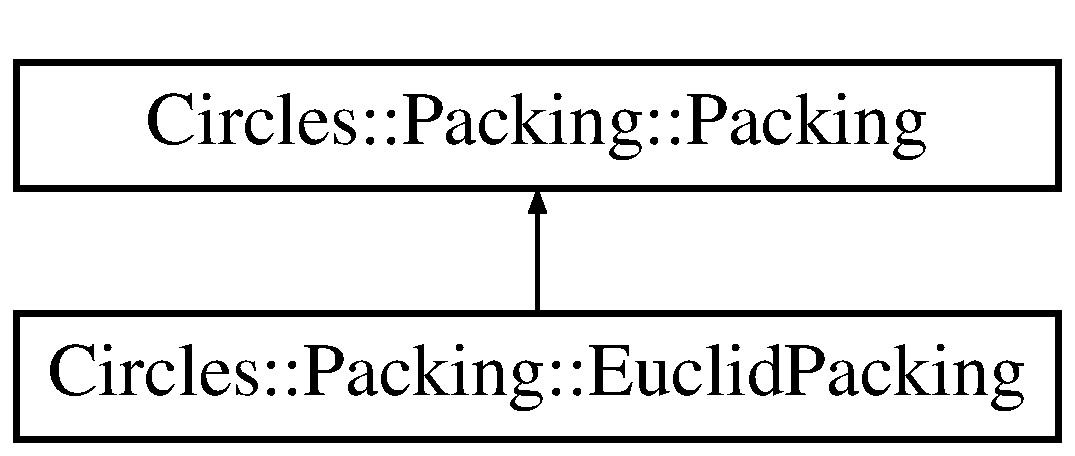
\includegraphics[height=2.000000cm]{class_circles_1_1_packing_1_1_packing}
\end{center}
\end{figure}
\subsection*{Public Member Functions}
\begin{DoxyCompactItemize}
\item 
virtual void \hyperlink{class_circles_1_1_packing_1_1_packing_a368eba2c988e6d42f6b9b41a17126121}{repack} (qreal epsilon, qreal outer\+Radius)=0
\item 
virtual void \hyperlink{class_circles_1_1_packing_1_1_packing_aad695ed5f3341f75ea7b2b4135203a7f}{layout} (int center\+Node)=0
\item 
virtual qreal \hyperlink{class_circles_1_1_packing_1_1_packing_a41991c2ef4010416fb382ae4e180e7ee}{angle} (const Q\+Point\+F \&p, const Q\+Point\+F \&p1, const Q\+Point\+F \&p2) const  =0
\item 
const \hyperlink{class_circles_1_1_graph_1_1_graph}{Graph\+::\+Graph} \& \hyperlink{class_circles_1_1_packing_1_1_packing_ab1da9320813d23d0b24e3ad67dcd6b03}{graph} () const 
\item 
Q\+Map$<$ int, \hyperlink{class_circles_1_1_packing_1_1_circle}{Circle} $\ast$ $>$ \hyperlink{class_circles_1_1_packing_1_1_packing_a6dec25e7a0fc0fee6e1f3fb7856a7867}{circles} () const 
\item 
const \hyperlink{class_circles_1_1_packing_1_1_circle}{Circle} $\ast$ \hyperlink{class_circles_1_1_packing_1_1_packing_ab4c423f23c7859f6c6fc93b0b2f2462c}{circle} (int index) const 
\end{DoxyCompactItemize}
\subsection*{Protected Member Functions}
\begin{DoxyCompactItemize}
\item 
qreal \hyperlink{class_circles_1_1_packing_1_1_packing_ae517dffd81c8526daf4d68dc556edb7a}{anglesum} (const \hyperlink{class_circles_1_1_packing_1_1_circle}{Circle} \&c) const 
\end{DoxyCompactItemize}
\subsection*{Protected Attributes}
\begin{DoxyCompactItemize}
\item 
std\+::shared\+\_\+ptr$<$ \hyperlink{class_circles_1_1_graph_1_1_graph}{Graph\+::\+Graph} $>$ \hyperlink{class_circles_1_1_packing_1_1_packing_aafdbbfa163315d47de5805b7eb55c549}{\+\_\+graph}
\item 
Q\+Map$<$ int, std\+::unique\+\_\+ptr$<$ \hyperlink{class_circles_1_1_packing_1_1_circle}{Circle} $>$ $>$ \hyperlink{class_circles_1_1_packing_1_1_packing_a34a1ece667f3111c1eb434ee7660b31a}{\+\_\+circles}
\end{DoxyCompactItemize}


\subsection{Detailed Description}
Abstract base class of the \hyperlink{class_circles_1_1_packing_1_1_euclid_packing}{Euclid\+Packing} and the Hyper\+Packing, which represent a circle packing over a specific \hyperlink{namespace_circles_1_1_graph}{Graph}.

\hyperlink{class_circles_1_1_packing_1_1_circle}{Circle} packings consist of a number of circles which lie tangent to eachother. 

\subsection{Member Function Documentation}
\hypertarget{class_circles_1_1_packing_1_1_packing_a41991c2ef4010416fb382ae4e180e7ee}{}\index{Circles\+::\+Packing\+::\+Packing@{Circles\+::\+Packing\+::\+Packing}!angle@{angle}}
\index{angle@{angle}!Circles\+::\+Packing\+::\+Packing@{Circles\+::\+Packing\+::\+Packing}}
\subsubsection[{angle(const Q\+Point\+F \&p, const Q\+Point\+F \&p1, const Q\+Point\+F \&p2) const  =0}]{\setlength{\rightskip}{0pt plus 5cm}virtual qreal Circles\+::\+Packing\+::\+Packing\+::angle (
\begin{DoxyParamCaption}
\item[{const Q\+Point\+F \&}]{p, }
\item[{const Q\+Point\+F \&}]{p1, }
\item[{const Q\+Point\+F \&}]{p2}
\end{DoxyParamCaption}
) const\hspace{0.3cm}{\ttfamily [pure virtual]}}\label{class_circles_1_1_packing_1_1_packing_a41991c2ef4010416fb382ae4e180e7ee}
Compute the angle $<$p,p1,p2 in the local space of the packing. 
\begin{DoxyParams}{Parameters}
{\em point} & which represents the vertex point. \\
\hline
{\em point} & which defines one ray of the angle. \\
\hline
{\em point} & which defines the other ray of the angle. \\
\hline
\end{DoxyParams}
\begin{DoxyReturn}{Returns}
The angle formed by the points, in radians in range \mbox{[}0, pi\mbox{]} 
\end{DoxyReturn}
\hypertarget{class_circles_1_1_packing_1_1_packing_ae517dffd81c8526daf4d68dc556edb7a}{}\index{Circles\+::\+Packing\+::\+Packing@{Circles\+::\+Packing\+::\+Packing}!anglesum@{anglesum}}
\index{anglesum@{anglesum}!Circles\+::\+Packing\+::\+Packing@{Circles\+::\+Packing\+::\+Packing}}
\subsubsection[{anglesum(const Circle \&c) const }]{\setlength{\rightskip}{0pt plus 5cm}qreal Packing\+::anglesum (
\begin{DoxyParamCaption}
\item[{const {\bf Circle} \&}]{c}
\end{DoxyParamCaption}
) const\hspace{0.3cm}{\ttfamily [protected]}}\label{class_circles_1_1_packing_1_1_packing_ae517dffd81c8526daf4d68dc556edb7a}
Compute the sum of the angles formed by a circle and its neighbours. 
\begin{DoxyParams}{Parameters}
{\em c} & the circle to consider. \\
\hline
\end{DoxyParams}
\begin{DoxyReturn}{Returns}
sum of angles in radians, in range \mbox{[}0, 2pi\mbox{]} 
\end{DoxyReturn}
\hypertarget{class_circles_1_1_packing_1_1_packing_ab4c423f23c7859f6c6fc93b0b2f2462c}{}\index{Circles\+::\+Packing\+::\+Packing@{Circles\+::\+Packing\+::\+Packing}!circle@{circle}}
\index{circle@{circle}!Circles\+::\+Packing\+::\+Packing@{Circles\+::\+Packing\+::\+Packing}}
\subsubsection[{circle(int index) const }]{\setlength{\rightskip}{0pt plus 5cm}const {\bf Circle} $\ast$ Packing\+::circle (
\begin{DoxyParamCaption}
\item[{int}]{index}
\end{DoxyParamCaption}
) const}\label{class_circles_1_1_packing_1_1_packing_ab4c423f23c7859f6c6fc93b0b2f2462c}
Get a circle based on its index. 
\begin{DoxyParams}{Parameters}
{\em index} & index of the circle \\
\hline
\end{DoxyParams}
\begin{DoxyReturn}{Returns}
const reference to circle with specified index. 
\end{DoxyReturn}
\hypertarget{class_circles_1_1_packing_1_1_packing_a6dec25e7a0fc0fee6e1f3fb7856a7867}{}\index{Circles\+::\+Packing\+::\+Packing@{Circles\+::\+Packing\+::\+Packing}!circles@{circles}}
\index{circles@{circles}!Circles\+::\+Packing\+::\+Packing@{Circles\+::\+Packing\+::\+Packing}}
\subsubsection[{circles() const }]{\setlength{\rightskip}{0pt plus 5cm}Q\+Map$<$ int, {\bf Circle} $\ast$ $>$ Packing\+::circles (
\begin{DoxyParamCaption}
{}
\end{DoxyParamCaption}
) const}\label{class_circles_1_1_packing_1_1_packing_a6dec25e7a0fc0fee6e1f3fb7856a7867}
Get a list of all circles in the packing, addressable by their indicies. \begin{DoxyReturn}{Returns}
Qhash of index -\/$>$ circle elements for the packing. 
\end{DoxyReturn}
\hypertarget{class_circles_1_1_packing_1_1_packing_ab1da9320813d23d0b24e3ad67dcd6b03}{}\index{Circles\+::\+Packing\+::\+Packing@{Circles\+::\+Packing\+::\+Packing}!graph@{graph}}
\index{graph@{graph}!Circles\+::\+Packing\+::\+Packing@{Circles\+::\+Packing\+::\+Packing}}
\subsubsection[{graph() const }]{\setlength{\rightskip}{0pt plus 5cm}const {\bf Graph\+::\+Graph} \& Packing\+::graph (
\begin{DoxyParamCaption}
{}
\end{DoxyParamCaption}
) const}\label{class_circles_1_1_packing_1_1_packing_ab1da9320813d23d0b24e3ad67dcd6b03}
Get a reference to the underlying graph of the packing. \begin{DoxyReturn}{Returns}
const reference to graph object underlying the packing. 
\end{DoxyReturn}
\hypertarget{class_circles_1_1_packing_1_1_packing_aad695ed5f3341f75ea7b2b4135203a7f}{}\index{Circles\+::\+Packing\+::\+Packing@{Circles\+::\+Packing\+::\+Packing}!layout@{layout}}
\index{layout@{layout}!Circles\+::\+Packing\+::\+Packing@{Circles\+::\+Packing\+::\+Packing}}
\subsubsection[{layout(int center\+Node)=0}]{\setlength{\rightskip}{0pt plus 5cm}virtual void Circles\+::\+Packing\+::\+Packing\+::layout (
\begin{DoxyParamCaption}
\item[{int}]{center\+Node}
\end{DoxyParamCaption}
)\hspace{0.3cm}{\ttfamily [pure virtual]}}\label{class_circles_1_1_packing_1_1_packing_aad695ed5f3341f75ea7b2b4135203a7f}
Lay out the circles such that neighbouring circles are tangent to one another. 
\begin{DoxyParams}{Parameters}
{\em center\+Node} & index of the circle to place at the center of the packing. \\
\hline
\end{DoxyParams}
\hypertarget{class_circles_1_1_packing_1_1_packing_a368eba2c988e6d42f6b9b41a17126121}{}\index{Circles\+::\+Packing\+::\+Packing@{Circles\+::\+Packing\+::\+Packing}!repack@{repack}}
\index{repack@{repack}!Circles\+::\+Packing\+::\+Packing@{Circles\+::\+Packing\+::\+Packing}}
\subsubsection[{repack(qreal epsilon, qreal outer\+Radius)=0}]{\setlength{\rightskip}{0pt plus 5cm}virtual void Circles\+::\+Packing\+::\+Packing\+::repack (
\begin{DoxyParamCaption}
\item[{qreal}]{epsilon, }
\item[{qreal}]{outer\+Radius}
\end{DoxyParamCaption}
)\hspace{0.3cm}{\ttfamily [pure virtual]}}\label{class_circles_1_1_packing_1_1_packing_a368eba2c988e6d42f6b9b41a17126121}
Set boundary circles to be of a specified radius and then modify other circles to form a proper packing. 
\begin{DoxyParams}{Parameters}
{\em epsilon} & tolerance value when determining angle sum \\
\hline
{\em outer\+Radius} & Radius of the boundary circles. \\
\hline
\end{DoxyParams}


\subsection{Member Data Documentation}
\hypertarget{class_circles_1_1_packing_1_1_packing_a34a1ece667f3111c1eb434ee7660b31a}{}\index{Circles\+::\+Packing\+::\+Packing@{Circles\+::\+Packing\+::\+Packing}!\+\_\+circles@{\+\_\+circles}}
\index{\+\_\+circles@{\+\_\+circles}!Circles\+::\+Packing\+::\+Packing@{Circles\+::\+Packing\+::\+Packing}}
\subsubsection[{\+\_\+circles}]{\setlength{\rightskip}{0pt plus 5cm}Q\+Map$<$int, std\+::unique\+\_\+ptr$<${\bf Circle}$>$ $>$ Circles\+::\+Packing\+::\+Packing\+::\+\_\+circles\hspace{0.3cm}{\ttfamily [protected]}}\label{class_circles_1_1_packing_1_1_packing_a34a1ece667f3111c1eb434ee7660b31a}
\hypertarget{class_circles_1_1_packing_1_1_packing_aafdbbfa163315d47de5805b7eb55c549}{}\index{Circles\+::\+Packing\+::\+Packing@{Circles\+::\+Packing\+::\+Packing}!\+\_\+graph@{\+\_\+graph}}
\index{\+\_\+graph@{\+\_\+graph}!Circles\+::\+Packing\+::\+Packing@{Circles\+::\+Packing\+::\+Packing}}
\subsubsection[{\+\_\+graph}]{\setlength{\rightskip}{0pt plus 5cm}std\+::shared\+\_\+ptr$<${\bf Graph\+::\+Graph}$>$ Circles\+::\+Packing\+::\+Packing\+::\+\_\+graph\hspace{0.3cm}{\ttfamily [protected]}}\label{class_circles_1_1_packing_1_1_packing_aafdbbfa163315d47de5805b7eb55c549}


The documentation for this class was generated from the following files\+:\begin{DoxyCompactItemize}
\item 
packing/\hyperlink{packing_2_packing_8hpp}{Packing.\+hpp}\item 
packing/\hyperlink{packing_2_packing_8cpp}{Packing.\+cpp}\end{DoxyCompactItemize}

\hypertarget{class_packing_view}{}\section{Packing\+View Class Reference}
\label{class_packing_view}\index{Packing\+View@{Packing\+View}}


{\ttfamily \#include $<$Packing\+View.\+hpp$>$}

Inheritance diagram for Packing\+View\+:\begin{figure}[H]
\begin{center}
\leavevmode
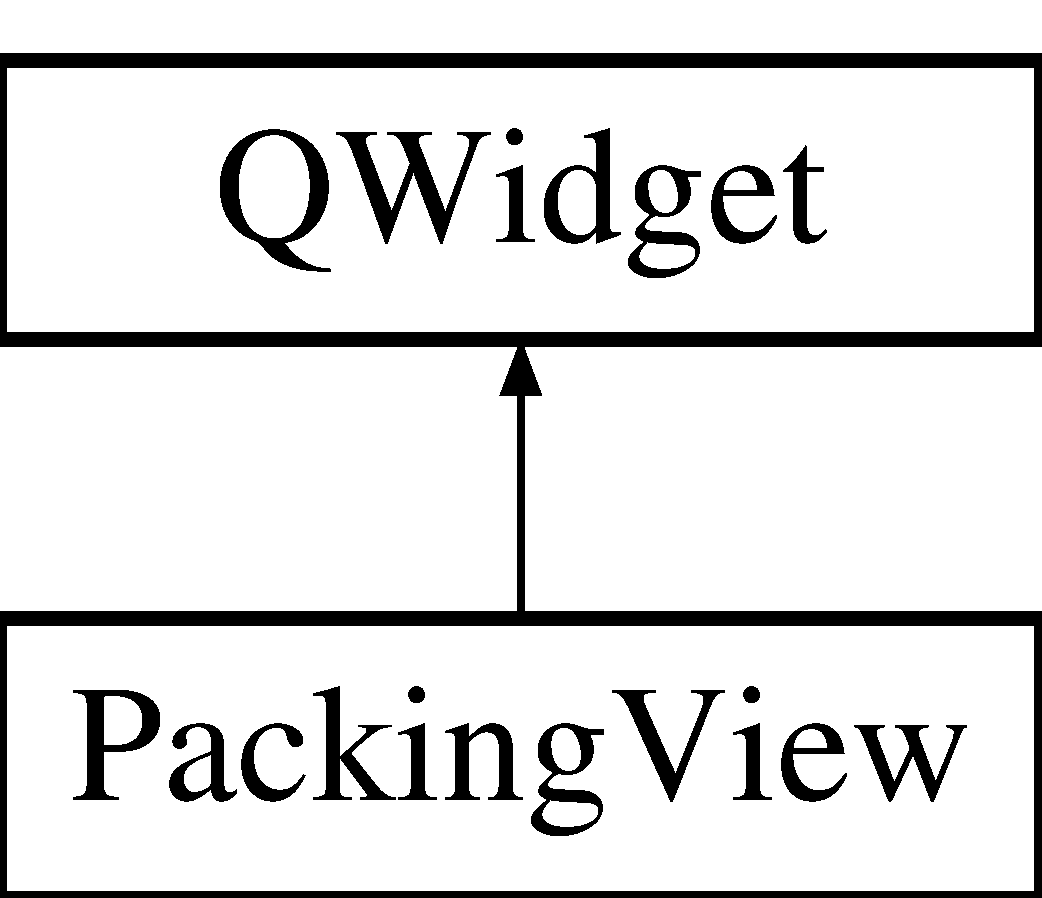
\includegraphics[height=2.000000cm]{class_packing_view}
\end{center}
\end{figure}
\subsection*{Public Slots}
\begin{DoxyCompactItemize}
\item 
void \hyperlink{class_packing_view_a5abe5e890fb107618ecffeba46445604}{set\+Packing} (\hyperlink{class_packing}{Packing} $\ast$p)
\end{DoxyCompactItemize}
\subsection*{Public Member Functions}
\begin{DoxyCompactItemize}
\item 
\hyperlink{class_packing_view_a110d5ad164b4d136814786060ae2627d}{Packing\+View} (Q\+Widget $\ast$parent=0)
\item 
\hyperlink{class_packing_view_ad93c70193ce437bcba4ceb9f51db05a2}{Packing\+View} (\hyperlink{class_packing}{Packing} $\ast$p, Q\+Widget $\ast$parent=0)
\item 
\hyperlink{class_packing_view_a443ae031c92775cb6bd2a579c5bd8d44}{$\sim$\+Packing\+View} ()
\end{DoxyCompactItemize}


\subsection{Constructor \& Destructor Documentation}
\hypertarget{class_packing_view_a110d5ad164b4d136814786060ae2627d}{}\index{Packing\+View@{Packing\+View}!Packing\+View@{Packing\+View}}
\index{Packing\+View@{Packing\+View}!Packing\+View@{Packing\+View}}
\subsubsection[{Packing\+View(\+Q\+Widget $\ast$parent=0)}]{\setlength{\rightskip}{0pt plus 5cm}Packing\+View\+::\+Packing\+View (
\begin{DoxyParamCaption}
\item[{Q\+Widget $\ast$}]{parent = {\ttfamily 0}}
\end{DoxyParamCaption}
)\hspace{0.3cm}{\ttfamily [explicit]}}\label{class_packing_view_a110d5ad164b4d136814786060ae2627d}
\hypertarget{class_packing_view_ad93c70193ce437bcba4ceb9f51db05a2}{}\index{Packing\+View@{Packing\+View}!Packing\+View@{Packing\+View}}
\index{Packing\+View@{Packing\+View}!Packing\+View@{Packing\+View}}
\subsubsection[{Packing\+View(\+Packing $\ast$p, Q\+Widget $\ast$parent=0)}]{\setlength{\rightskip}{0pt plus 5cm}Packing\+View\+::\+Packing\+View (
\begin{DoxyParamCaption}
\item[{{\bf Packing} $\ast$}]{p, }
\item[{Q\+Widget $\ast$}]{parent = {\ttfamily 0}}
\end{DoxyParamCaption}
)}\label{class_packing_view_ad93c70193ce437bcba4ceb9f51db05a2}
\hypertarget{class_packing_view_a443ae031c92775cb6bd2a579c5bd8d44}{}\index{Packing\+View@{Packing\+View}!````~Packing\+View@{$\sim$\+Packing\+View}}
\index{````~Packing\+View@{$\sim$\+Packing\+View}!Packing\+View@{Packing\+View}}
\subsubsection[{$\sim$\+Packing\+View()}]{\setlength{\rightskip}{0pt plus 5cm}Packing\+View\+::$\sim$\+Packing\+View (
\begin{DoxyParamCaption}
{}
\end{DoxyParamCaption}
)}\label{class_packing_view_a443ae031c92775cb6bd2a579c5bd8d44}


\subsection{Member Function Documentation}
\hypertarget{class_packing_view_a5abe5e890fb107618ecffeba46445604}{}\index{Packing\+View@{Packing\+View}!set\+Packing@{set\+Packing}}
\index{set\+Packing@{set\+Packing}!Packing\+View@{Packing\+View}}
\subsubsection[{set\+Packing}]{\setlength{\rightskip}{0pt plus 5cm}void Packing\+View\+::set\+Packing (
\begin{DoxyParamCaption}
\item[{{\bf Packing} $\ast$}]{p}
\end{DoxyParamCaption}
)\hspace{0.3cm}{\ttfamily [slot]}}\label{class_packing_view_a5abe5e890fb107618ecffeba46445604}


The documentation for this class was generated from the following files\+:\begin{DoxyCompactItemize}
\item 
ui/\hyperlink{_packing_view_8hpp}{Packing\+View.\+hpp}\item 
ui/\hyperlink{_packing_view_8cpp}{Packing\+View.\+cpp}\end{DoxyCompactItemize}

\hypertarget{class_p_file}{}\section{P\+File Class Reference}
\label{class_p_file}\index{P\+File@{P\+File}}


{\ttfamily \#include $<$P\+File.\+hpp$>$}

\subsection*{Public Member Functions}
\begin{DoxyCompactItemize}
\item 
\hyperlink{class_p_file_af35ac6cc8fd2e3f9131bbd65fdb8a434}{P\+File} (Q\+String filename)
\item 
\hyperlink{class_packing}{Packing} $\ast$ \hyperlink{class_p_file_ace04e8c342cbc29d1a09544b728caada}{generate\+Packing} ()
\end{DoxyCompactItemize}


\subsection{Constructor \& Destructor Documentation}
\hypertarget{class_p_file_af35ac6cc8fd2e3f9131bbd65fdb8a434}{}\index{P\+File@{P\+File}!P\+File@{P\+File}}
\index{P\+File@{P\+File}!P\+File@{P\+File}}
\subsubsection[{P\+File(\+Q\+String filename)}]{\setlength{\rightskip}{0pt plus 5cm}P\+File\+::\+P\+File (
\begin{DoxyParamCaption}
\item[{Q\+String}]{filename}
\end{DoxyParamCaption}
)}\label{class_p_file_af35ac6cc8fd2e3f9131bbd65fdb8a434}


\subsection{Member Function Documentation}
\hypertarget{class_p_file_ace04e8c342cbc29d1a09544b728caada}{}\index{P\+File@{P\+File}!generate\+Packing@{generate\+Packing}}
\index{generate\+Packing@{generate\+Packing}!P\+File@{P\+File}}
\subsubsection[{generate\+Packing()}]{\setlength{\rightskip}{0pt plus 5cm}{\bf Packing} $\ast$ P\+File\+::generate\+Packing (
\begin{DoxyParamCaption}
{}
\end{DoxyParamCaption}
)}\label{class_p_file_ace04e8c342cbc29d1a09544b728caada}


The documentation for this class was generated from the following files\+:\begin{DoxyCompactItemize}
\item 
\hyperlink{_p_file_8hpp}{P\+File.\+hpp}\item 
\hyperlink{_p_file_8cpp}{P\+File.\+cpp}\end{DoxyCompactItemize}

\hypertarget{class_property_window}{}\section{Property\+Window Class Reference}
\label{class_property_window}\index{Property\+Window@{Property\+Window}}


{\ttfamily \#include $<$Property\+Window.\+hpp$>$}

Inheritance diagram for Property\+Window\+:\begin{figure}[H]
\begin{center}
\leavevmode
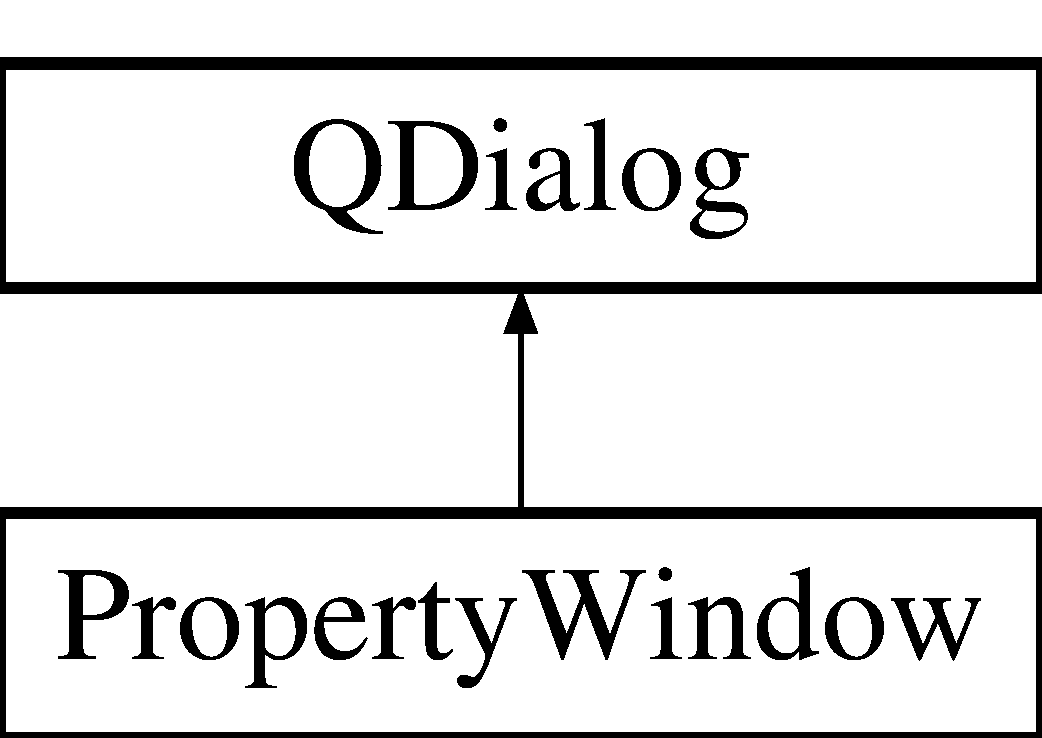
\includegraphics[height=2.000000cm]{class_property_window}
\end{center}
\end{figure}
\subsection*{Public Slots}
\begin{DoxyCompactItemize}
\item 
void \hyperlink{class_property_window_a9cf01fbc71ed7f8272933dabeddc9e5f}{set\+Node} (\hyperlink{class_node}{Node} $\ast$n)
\item 
void \hyperlink{class_property_window_ad47ff8214d08fe5e7b8555c849224a93}{refresh} ()
\end{DoxyCompactItemize}
\subsection*{Public Member Functions}
\begin{DoxyCompactItemize}
\item 
\hyperlink{class_property_window_a64e1485e298f164b03ab49f00ce0295b}{Property\+Window} (Q\+Widget $\ast$parent=0)
\item 
\hyperlink{class_property_window_ae6d801af2d3ffc2c1de031da20d5dd6a}{$\sim$\+Property\+Window} ()
\end{DoxyCompactItemize}


\subsection{Constructor \& Destructor Documentation}
\hypertarget{class_property_window_a64e1485e298f164b03ab49f00ce0295b}{}\index{Property\+Window@{Property\+Window}!Property\+Window@{Property\+Window}}
\index{Property\+Window@{Property\+Window}!Property\+Window@{Property\+Window}}
\subsubsection[{Property\+Window(\+Q\+Widget $\ast$parent=0)}]{\setlength{\rightskip}{0pt plus 5cm}Property\+Window\+::\+Property\+Window (
\begin{DoxyParamCaption}
\item[{Q\+Widget $\ast$}]{parent = {\ttfamily 0}}
\end{DoxyParamCaption}
)\hspace{0.3cm}{\ttfamily [explicit]}}\label{class_property_window_a64e1485e298f164b03ab49f00ce0295b}
\hypertarget{class_property_window_ae6d801af2d3ffc2c1de031da20d5dd6a}{}\index{Property\+Window@{Property\+Window}!````~Property\+Window@{$\sim$\+Property\+Window}}
\index{````~Property\+Window@{$\sim$\+Property\+Window}!Property\+Window@{Property\+Window}}
\subsubsection[{$\sim$\+Property\+Window()}]{\setlength{\rightskip}{0pt plus 5cm}Property\+Window\+::$\sim$\+Property\+Window (
\begin{DoxyParamCaption}
{}
\end{DoxyParamCaption}
)}\label{class_property_window_ae6d801af2d3ffc2c1de031da20d5dd6a}


\subsection{Member Function Documentation}
\hypertarget{class_property_window_ad47ff8214d08fe5e7b8555c849224a93}{}\index{Property\+Window@{Property\+Window}!refresh@{refresh}}
\index{refresh@{refresh}!Property\+Window@{Property\+Window}}
\subsubsection[{refresh}]{\setlength{\rightskip}{0pt plus 5cm}void Property\+Window\+::refresh (
\begin{DoxyParamCaption}
{}
\end{DoxyParamCaption}
)\hspace{0.3cm}{\ttfamily [slot]}}\label{class_property_window_ad47ff8214d08fe5e7b8555c849224a93}
Updates the visual display using information from the currently selected node. \hypertarget{class_property_window_a9cf01fbc71ed7f8272933dabeddc9e5f}{}\index{Property\+Window@{Property\+Window}!set\+Node@{set\+Node}}
\index{set\+Node@{set\+Node}!Property\+Window@{Property\+Window}}
\subsubsection[{set\+Node}]{\setlength{\rightskip}{0pt plus 5cm}void Property\+Window\+::set\+Node (
\begin{DoxyParamCaption}
\item[{{\bf Node} $\ast$}]{n}
\end{DoxyParamCaption}
)\hspace{0.3cm}{\ttfamily [slot]}}\label{class_property_window_a9cf01fbc71ed7f8272933dabeddc9e5f}
Sets the node which is displayed in the property window. 
\begin{DoxyParams}{Parameters}
{\em n} & \hyperlink{class_node}{Node} to display. \\
\hline
\end{DoxyParams}


The documentation for this class was generated from the following files\+:\begin{DoxyCompactItemize}
\item 
ui/\hyperlink{_property_window_8hpp}{Property\+Window.\+hpp}\item 
ui/\hyperlink{_property_window_8cpp}{Property\+Window.\+cpp}\end{DoxyCompactItemize}

\hypertarget{class_selection_packing}{}\section{Selection\+Packing Class Reference}
\label{class_selection_packing}\index{Selection\+Packing@{Selection\+Packing}}


{\ttfamily \#include $<$Selection\+Packing.\+hpp$>$}

Inheritance diagram for Selection\+Packing\+:\begin{figure}[H]
\begin{center}
\leavevmode
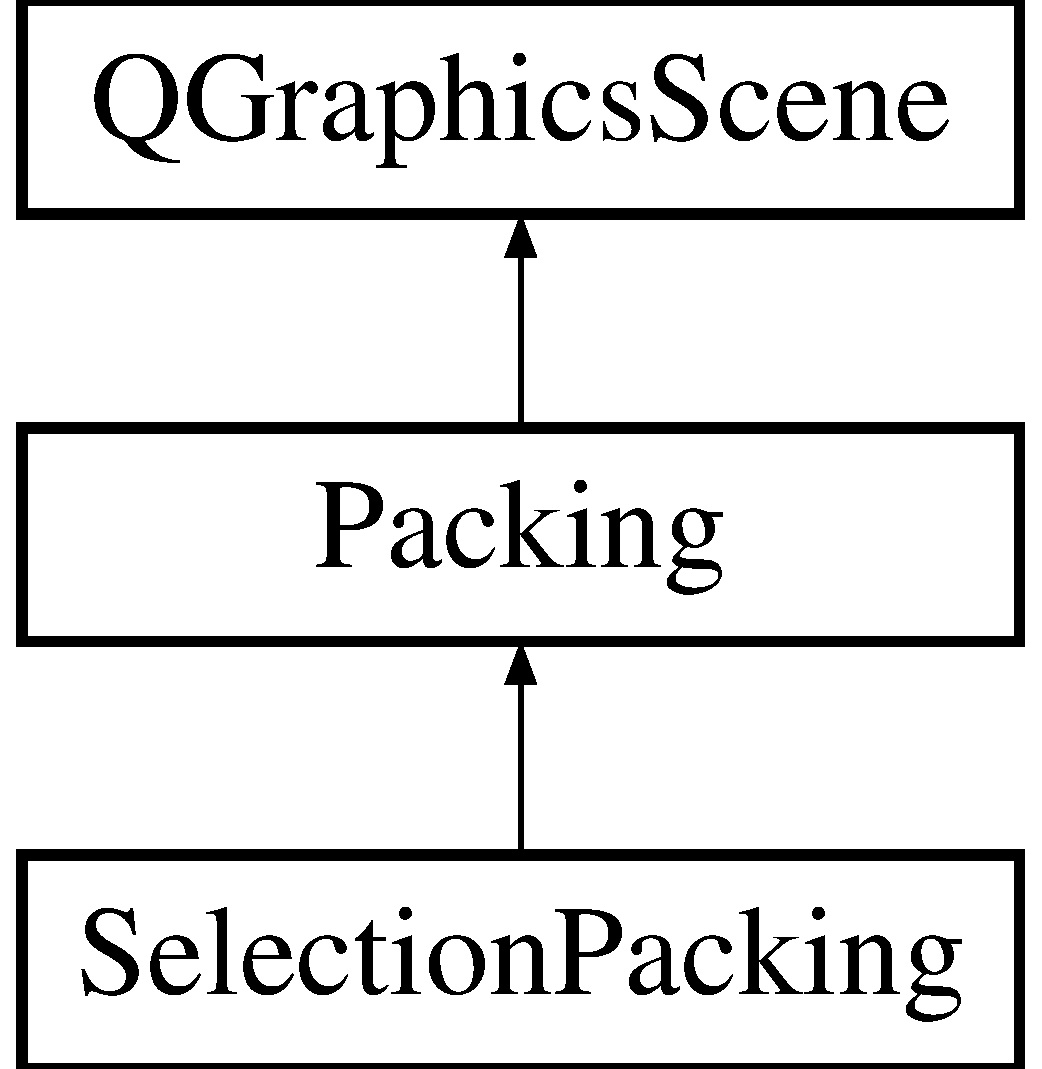
\includegraphics[height=3.000000cm]{class_selection_packing}
\end{center}
\end{figure}
\subsection*{Public Types}
\begin{DoxyCompactItemize}
\item 
enum \hyperlink{class_selection_packing_a34fc2fbb6a758004b3b19d7c73997241}{Mouse\+Mode} \{ \hyperlink{class_selection_packing_a34fc2fbb6a758004b3b19d7c73997241a6adf97f83acf6453d4a6a4b1070f3754}{Mouse\+Mode\+::\+None}, 
\hyperlink{class_selection_packing_a34fc2fbb6a758004b3b19d7c73997241aec211f7c20af43e742bf2570c3cb84f9}{Mouse\+Mode\+::\+Add}, 
\hyperlink{class_selection_packing_a34fc2fbb6a758004b3b19d7c73997241a1d9baf077ee87921f57a8fe42d510b65}{Mouse\+Mode\+::\+Subtract}
 \}
\end{DoxyCompactItemize}
\subsection*{Public Member Functions}
\begin{DoxyCompactItemize}
\item 
\hyperlink{class_selection_packing_a02c377676ebd303632c41b0e60725bf4}{Selection\+Packing} (\hyperlink{graphics_2_packing_8hpp_a331874350131c9e1039dac50b427f8b9}{Packing\+Type} \hyperlink{class_packing_a934cbe1ef81173f5e7fbabf9846d16e2}{type}=\hyperlink{graphics_2_packing_8hpp_a331874350131c9e1039dac50b427f8b9aa4066bbe6791ed6bbfe12f55a60ed152}{Packing\+Type\+::\+Euclidean\+Packing})
\item 
\hyperlink{class_selection_packing_a22e56f099a555fb00e4726e9b019be60}{Selection\+Packing} (Q\+List$<$ \hyperlink{class_node}{Node} $\ast$ $>$ \hyperlink{class_packing_afee4e76e75aea147685840e19c714d08}{nodes}, \hyperlink{graphics_2_packing_8hpp_a331874350131c9e1039dac50b427f8b9}{Packing\+Type} \hyperlink{class_packing_a934cbe1ef81173f5e7fbabf9846d16e2}{type}=\hyperlink{graphics_2_packing_8hpp_a331874350131c9e1039dac50b427f8b9af44d305ffa405b64040c7d4bc16953f9}{Packing\+Type\+::\+Hyperbolic\+Packing})
\item 
bool \hyperlink{class_selection_packing_a0a3dd7c75b32c883914c660042d3ed0b}{add\+To\+Selection} (\hyperlink{class_circle}{Circle} $\ast$c)
\begin{DoxyCompactList}\small\item\em Attempts to add a circle c to the collection of selected circles If a previous circle is in the selection and the new circle is not ajacent to that circle, then the circle will not be added. \end{DoxyCompactList}\item 
void \hyperlink{class_selection_packing_ae29608e25fcfa2bfd485c8adfc941a46}{remove\+From\+Selection} (\hyperlink{class_circle}{Circle} $\ast$c)
\item 
bool \hyperlink{class_selection_packing_a9568899d6773f596e7d679f2a50bfc8d}{is\+In\+Selection} (\hyperlink{class_circle}{Circle} $\ast$c)
\item 
void \hyperlink{class_selection_packing_a04d54c3f7efbc412756f0b775d8aef8e}{clear\+Selection} ()
\item 
void \hyperlink{class_selection_packing_a424e907d2394d6b7d5941a10f6119cbc}{mouse\+Press\+Event} (Q\+Graphics\+Scene\+Mouse\+Event $\ast$mouse\+Event) Q\+\_\+\+D\+E\+C\+L\+\_\+\+O\+V\+E\+R\+R\+I\+D\+E
\item 
void \hyperlink{class_selection_packing_a7da53f29f45ccb15816b74033e307f1e}{mouse\+Move\+Event} (Q\+Graphics\+Scene\+Mouse\+Event $\ast$event) Q\+\_\+\+D\+E\+C\+L\+\_\+\+O\+V\+E\+R\+R\+I\+D\+E
\item 
void \hyperlink{class_selection_packing_ac8acca567094473a7957e634c75293f3}{mouse\+Release\+Event} (Q\+Graphics\+Scene\+Mouse\+Event $\ast$event) Q\+\_\+\+D\+E\+C\+L\+\_\+\+O\+V\+E\+R\+R\+I\+D\+E
\end{DoxyCompactItemize}
\subsection*{Additional Inherited Members}


\subsection{Member Enumeration Documentation}
\hypertarget{class_selection_packing_a34fc2fbb6a758004b3b19d7c73997241}{}\index{Selection\+Packing@{Selection\+Packing}!Mouse\+Mode@{Mouse\+Mode}}
\index{Mouse\+Mode@{Mouse\+Mode}!Selection\+Packing@{Selection\+Packing}}
\subsubsection[{Mouse\+Mode}]{\setlength{\rightskip}{0pt plus 5cm}enum {\bf Selection\+Packing\+::\+Mouse\+Mode}\hspace{0.3cm}{\ttfamily [strong]}}\label{class_selection_packing_a34fc2fbb6a758004b3b19d7c73997241}
\begin{Desc}
\item[Enumerator]\par
\begin{description}
\index{None@{None}!Selection\+Packing@{Selection\+Packing}}\index{Selection\+Packing@{Selection\+Packing}!None@{None}}\item[{\em 
\hypertarget{class_selection_packing_a34fc2fbb6a758004b3b19d7c73997241a6adf97f83acf6453d4a6a4b1070f3754}{}None\label{class_selection_packing_a34fc2fbb6a758004b3b19d7c73997241a6adf97f83acf6453d4a6a4b1070f3754}
}]\index{Add@{Add}!Selection\+Packing@{Selection\+Packing}}\index{Selection\+Packing@{Selection\+Packing}!Add@{Add}}\item[{\em 
\hypertarget{class_selection_packing_a34fc2fbb6a758004b3b19d7c73997241aec211f7c20af43e742bf2570c3cb84f9}{}Add\label{class_selection_packing_a34fc2fbb6a758004b3b19d7c73997241aec211f7c20af43e742bf2570c3cb84f9}
}]\index{Subtract@{Subtract}!Selection\+Packing@{Selection\+Packing}}\index{Selection\+Packing@{Selection\+Packing}!Subtract@{Subtract}}\item[{\em 
\hypertarget{class_selection_packing_a34fc2fbb6a758004b3b19d7c73997241a1d9baf077ee87921f57a8fe42d510b65}{}Subtract\label{class_selection_packing_a34fc2fbb6a758004b3b19d7c73997241a1d9baf077ee87921f57a8fe42d510b65}
}]\end{description}
\end{Desc}


\subsection{Constructor \& Destructor Documentation}
\hypertarget{class_selection_packing_a02c377676ebd303632c41b0e60725bf4}{}\index{Selection\+Packing@{Selection\+Packing}!Selection\+Packing@{Selection\+Packing}}
\index{Selection\+Packing@{Selection\+Packing}!Selection\+Packing@{Selection\+Packing}}
\subsubsection[{Selection\+Packing(\+Packing\+Type type=\+Packing\+Type\+::\+Euclidean\+Packing)}]{\setlength{\rightskip}{0pt plus 5cm}Selection\+Packing\+::\+Selection\+Packing (
\begin{DoxyParamCaption}
\item[{{\bf Packing\+Type}}]{type = {\ttfamily {\bf Packing\+Type\+::\+Euclidean\+Packing}}}
\end{DoxyParamCaption}
)}\label{class_selection_packing_a02c377676ebd303632c41b0e60725bf4}
\hypertarget{class_selection_packing_a22e56f099a555fb00e4726e9b019be60}{}\index{Selection\+Packing@{Selection\+Packing}!Selection\+Packing@{Selection\+Packing}}
\index{Selection\+Packing@{Selection\+Packing}!Selection\+Packing@{Selection\+Packing}}
\subsubsection[{Selection\+Packing(\+Q\+List$<$ Node $\ast$ $>$ nodes, Packing\+Type type=\+Packing\+Type\+::\+Hyperbolic\+Packing)}]{\setlength{\rightskip}{0pt plus 5cm}Selection\+Packing\+::\+Selection\+Packing (
\begin{DoxyParamCaption}
\item[{Q\+List$<$ {\bf Node} $\ast$ $>$}]{nodes, }
\item[{{\bf Packing\+Type}}]{type = {\ttfamily {\bf Packing\+Type\+::\+Hyperbolic\+Packing}}}
\end{DoxyParamCaption}
)}\label{class_selection_packing_a22e56f099a555fb00e4726e9b019be60}


\subsection{Member Function Documentation}
\hypertarget{class_selection_packing_a0a3dd7c75b32c883914c660042d3ed0b}{}\index{Selection\+Packing@{Selection\+Packing}!add\+To\+Selection@{add\+To\+Selection}}
\index{add\+To\+Selection@{add\+To\+Selection}!Selection\+Packing@{Selection\+Packing}}
\subsubsection[{add\+To\+Selection(\+Circle $\ast$c)}]{\setlength{\rightskip}{0pt plus 5cm}bool Selection\+Packing\+::add\+To\+Selection (
\begin{DoxyParamCaption}
\item[{{\bf Circle} $\ast$}]{c}
\end{DoxyParamCaption}
)}\label{class_selection_packing_a0a3dd7c75b32c883914c660042d3ed0b}


Attempts to add a circle c to the collection of selected circles If a previous circle is in the selection and the new circle is not ajacent to that circle, then the circle will not be added. 


\begin{DoxyParams}{Parameters}
{\em c} & \\
\hline
\end{DoxyParams}
\begin{DoxyReturn}{Returns}

\end{DoxyReturn}
\hypertarget{class_selection_packing_a04d54c3f7efbc412756f0b775d8aef8e}{}\index{Selection\+Packing@{Selection\+Packing}!clear\+Selection@{clear\+Selection}}
\index{clear\+Selection@{clear\+Selection}!Selection\+Packing@{Selection\+Packing}}
\subsubsection[{clear\+Selection()}]{\setlength{\rightskip}{0pt plus 5cm}void Selection\+Packing\+::clear\+Selection (
\begin{DoxyParamCaption}
{}
\end{DoxyParamCaption}
)}\label{class_selection_packing_a04d54c3f7efbc412756f0b775d8aef8e}
\hypertarget{class_selection_packing_a9568899d6773f596e7d679f2a50bfc8d}{}\index{Selection\+Packing@{Selection\+Packing}!is\+In\+Selection@{is\+In\+Selection}}
\index{is\+In\+Selection@{is\+In\+Selection}!Selection\+Packing@{Selection\+Packing}}
\subsubsection[{is\+In\+Selection(\+Circle $\ast$c)}]{\setlength{\rightskip}{0pt plus 5cm}bool Selection\+Packing\+::is\+In\+Selection (
\begin{DoxyParamCaption}
\item[{{\bf Circle} $\ast$}]{c}
\end{DoxyParamCaption}
)}\label{class_selection_packing_a9568899d6773f596e7d679f2a50bfc8d}
\hypertarget{class_selection_packing_a7da53f29f45ccb15816b74033e307f1e}{}\index{Selection\+Packing@{Selection\+Packing}!mouse\+Move\+Event@{mouse\+Move\+Event}}
\index{mouse\+Move\+Event@{mouse\+Move\+Event}!Selection\+Packing@{Selection\+Packing}}
\subsubsection[{mouse\+Move\+Event(\+Q\+Graphics\+Scene\+Mouse\+Event $\ast$event) Q\+\_\+\+D\+E\+C\+L\+\_\+\+O\+V\+E\+R\+R\+I\+D\+E}]{\setlength{\rightskip}{0pt plus 5cm}void Selection\+Packing\+::mouse\+Move\+Event (
\begin{DoxyParamCaption}
\item[{Q\+Graphics\+Scene\+Mouse\+Event $\ast$}]{event}
\end{DoxyParamCaption}
)}\label{class_selection_packing_a7da53f29f45ccb15816b74033e307f1e}
\hypertarget{class_selection_packing_a424e907d2394d6b7d5941a10f6119cbc}{}\index{Selection\+Packing@{Selection\+Packing}!mouse\+Press\+Event@{mouse\+Press\+Event}}
\index{mouse\+Press\+Event@{mouse\+Press\+Event}!Selection\+Packing@{Selection\+Packing}}
\subsubsection[{mouse\+Press\+Event(\+Q\+Graphics\+Scene\+Mouse\+Event $\ast$mouse\+Event) Q\+\_\+\+D\+E\+C\+L\+\_\+\+O\+V\+E\+R\+R\+I\+D\+E}]{\setlength{\rightskip}{0pt plus 5cm}void Selection\+Packing\+::mouse\+Press\+Event (
\begin{DoxyParamCaption}
\item[{Q\+Graphics\+Scene\+Mouse\+Event $\ast$}]{mouse\+Event}
\end{DoxyParamCaption}
)\hspace{0.3cm}{\ttfamily [virtual]}}\label{class_selection_packing_a424e907d2394d6b7d5941a10f6119cbc}


Reimplemented from \hyperlink{class_packing_a6e130881196259c6594dd4bb2e96da4f}{Packing}.

\hypertarget{class_selection_packing_ac8acca567094473a7957e634c75293f3}{}\index{Selection\+Packing@{Selection\+Packing}!mouse\+Release\+Event@{mouse\+Release\+Event}}
\index{mouse\+Release\+Event@{mouse\+Release\+Event}!Selection\+Packing@{Selection\+Packing}}
\subsubsection[{mouse\+Release\+Event(\+Q\+Graphics\+Scene\+Mouse\+Event $\ast$event) Q\+\_\+\+D\+E\+C\+L\+\_\+\+O\+V\+E\+R\+R\+I\+D\+E}]{\setlength{\rightskip}{0pt plus 5cm}void Selection\+Packing\+::mouse\+Release\+Event (
\begin{DoxyParamCaption}
\item[{Q\+Graphics\+Scene\+Mouse\+Event $\ast$}]{event}
\end{DoxyParamCaption}
)}\label{class_selection_packing_ac8acca567094473a7957e634c75293f3}
\hypertarget{class_selection_packing_ae29608e25fcfa2bfd485c8adfc941a46}{}\index{Selection\+Packing@{Selection\+Packing}!remove\+From\+Selection@{remove\+From\+Selection}}
\index{remove\+From\+Selection@{remove\+From\+Selection}!Selection\+Packing@{Selection\+Packing}}
\subsubsection[{remove\+From\+Selection(\+Circle $\ast$c)}]{\setlength{\rightskip}{0pt plus 5cm}void Selection\+Packing\+::remove\+From\+Selection (
\begin{DoxyParamCaption}
\item[{{\bf Circle} $\ast$}]{c}
\end{DoxyParamCaption}
)}\label{class_selection_packing_ae29608e25fcfa2bfd485c8adfc941a46}


The documentation for this class was generated from the following files\+:\begin{DoxyCompactItemize}
\item 
graphics/\hyperlink{_selection_packing_8hpp}{Selection\+Packing.\+hpp}\item 
graphics/\hyperlink{_selection_packing_8cpp}{Selection\+Packing.\+cpp}\end{DoxyCompactItemize}

\hypertarget{class_selection_vertex}{}\section{Selection\+Vertex Class Reference}
\label{class_selection_vertex}\index{Selection\+Vertex@{Selection\+Vertex}}


{\ttfamily \#include $<$Selection\+Vertex.\+hpp$>$}

Inheritance diagram for Selection\+Vertex\+:\begin{figure}[H]
\begin{center}
\leavevmode
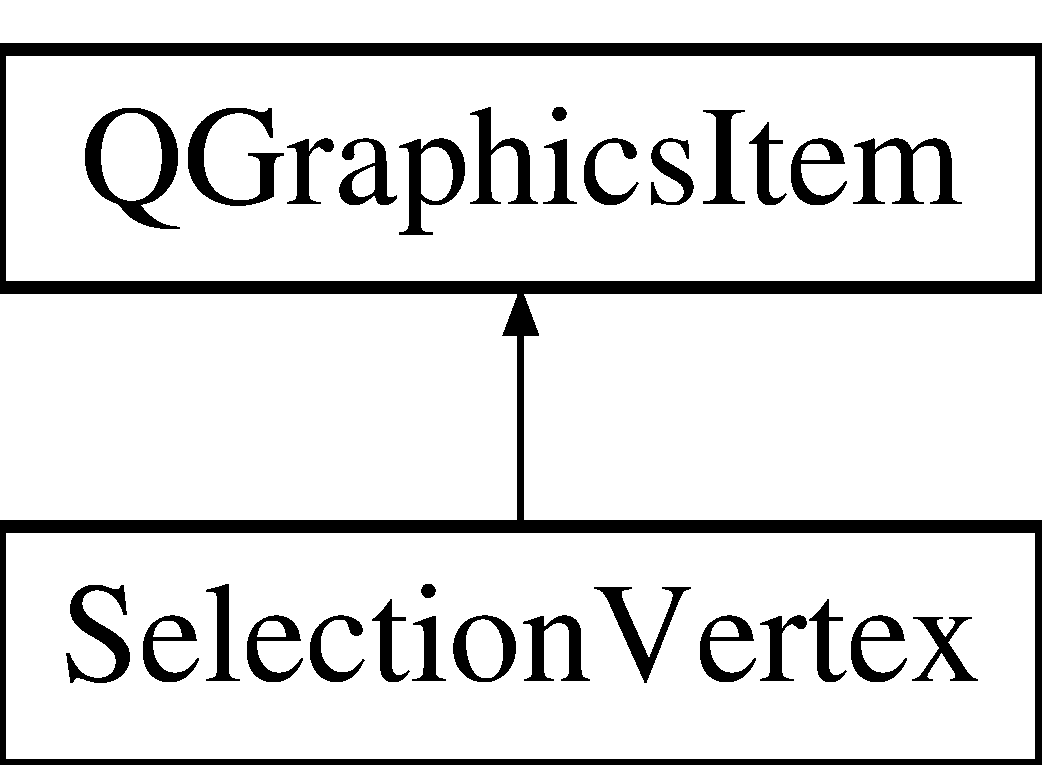
\includegraphics[height=2.000000cm]{class_selection_vertex}
\end{center}
\end{figure}
\subsection*{Public Member Functions}
\begin{DoxyCompactItemize}
\item 
\hyperlink{class_selection_vertex_acb10ca35d56e0606acdcb9c8a6342925}{Selection\+Vertex} (Q\+Point\+F position, Q\+Color color=Q\+Color(255, 0, 0))
\item 
Q\+Rect\+F \hyperlink{class_selection_vertex_aa9b0fc297965a721b4d29e48d5b628ac}{bounding\+Rect} () const Q\+\_\+\+D\+E\+C\+L\+\_\+\+O\+V\+E\+R\+R\+I\+D\+E
\item 
void \hyperlink{class_selection_vertex_a15246935fd481899f72834fb66b1314b}{paint} (Q\+Painter $\ast$painter, const Q\+Style\+Option\+Graphics\+Item $\ast$option, Q\+Widget $\ast$widget) Q\+\_\+\+D\+E\+C\+L\+\_\+\+O\+V\+E\+R\+R\+I\+D\+E
\end{DoxyCompactItemize}
\subsection*{Static Public Attributes}
\begin{DoxyCompactItemize}
\item 
static const qreal \hyperlink{class_selection_vertex_a618a13a2140b769bb44d4a8324d934fd}{size} = 15
\item 
static const qreal \hyperlink{class_selection_vertex_a8360abe25bea5202a7479637c30d60af}{thickness} = 3
\end{DoxyCompactItemize}


\subsection{Detailed Description}
Class which represents a selected vertex in the shape selector view. 

\subsection{Constructor \& Destructor Documentation}
\hypertarget{class_selection_vertex_acb10ca35d56e0606acdcb9c8a6342925}{}\index{Selection\+Vertex@{Selection\+Vertex}!Selection\+Vertex@{Selection\+Vertex}}
\index{Selection\+Vertex@{Selection\+Vertex}!Selection\+Vertex@{Selection\+Vertex}}
\subsubsection[{Selection\+Vertex(\+Q\+Point\+F position, Q\+Color color=\+Q\+Color(255, 0, 0))}]{\setlength{\rightskip}{0pt plus 5cm}Selection\+Vertex\+::\+Selection\+Vertex (
\begin{DoxyParamCaption}
\item[{Q\+Point\+F}]{position, }
\item[{Q\+Color}]{color = {\ttfamily QColor(255,~0,~0)}}
\end{DoxyParamCaption}
)}\label{class_selection_vertex_acb10ca35d56e0606acdcb9c8a6342925}


\subsection{Member Function Documentation}
\hypertarget{class_selection_vertex_aa9b0fc297965a721b4d29e48d5b628ac}{}\index{Selection\+Vertex@{Selection\+Vertex}!bounding\+Rect@{bounding\+Rect}}
\index{bounding\+Rect@{bounding\+Rect}!Selection\+Vertex@{Selection\+Vertex}}
\subsubsection[{bounding\+Rect() const Q\+\_\+\+D\+E\+C\+L\+\_\+\+O\+V\+E\+R\+R\+I\+D\+E}]{\setlength{\rightskip}{0pt plus 5cm}Q\+Rect\+F Selection\+Vertex\+::bounding\+Rect (
\begin{DoxyParamCaption}
{}
\end{DoxyParamCaption}
) const}\label{class_selection_vertex_aa9b0fc297965a721b4d29e48d5b628ac}
\hypertarget{class_selection_vertex_a15246935fd481899f72834fb66b1314b}{}\index{Selection\+Vertex@{Selection\+Vertex}!paint@{paint}}
\index{paint@{paint}!Selection\+Vertex@{Selection\+Vertex}}
\subsubsection[{paint(\+Q\+Painter $\ast$painter, const Q\+Style\+Option\+Graphics\+Item $\ast$option, Q\+Widget $\ast$widget) Q\+\_\+\+D\+E\+C\+L\+\_\+\+O\+V\+E\+R\+R\+I\+D\+E}]{\setlength{\rightskip}{0pt plus 5cm}void Selection\+Vertex\+::paint (
\begin{DoxyParamCaption}
\item[{Q\+Painter $\ast$}]{painter, }
\item[{const Q\+Style\+Option\+Graphics\+Item $\ast$}]{option, }
\item[{Q\+Widget $\ast$}]{widget}
\end{DoxyParamCaption}
)}\label{class_selection_vertex_a15246935fd481899f72834fb66b1314b}


\subsection{Member Data Documentation}
\hypertarget{class_selection_vertex_a618a13a2140b769bb44d4a8324d934fd}{}\index{Selection\+Vertex@{Selection\+Vertex}!size@{size}}
\index{size@{size}!Selection\+Vertex@{Selection\+Vertex}}
\subsubsection[{size}]{\setlength{\rightskip}{0pt plus 5cm}const qreal Selection\+Vertex\+::size = 15\hspace{0.3cm}{\ttfamily [static]}}\label{class_selection_vertex_a618a13a2140b769bb44d4a8324d934fd}
\hypertarget{class_selection_vertex_a8360abe25bea5202a7479637c30d60af}{}\index{Selection\+Vertex@{Selection\+Vertex}!thickness@{thickness}}
\index{thickness@{thickness}!Selection\+Vertex@{Selection\+Vertex}}
\subsubsection[{thickness}]{\setlength{\rightskip}{0pt plus 5cm}const qreal Selection\+Vertex\+::thickness = 3\hspace{0.3cm}{\ttfamily [static]}}\label{class_selection_vertex_a8360abe25bea5202a7479637c30d60af}


The documentation for this class was generated from the following files\+:\begin{DoxyCompactItemize}
\item 
graphics/\hyperlink{_selection_vertex_8hpp}{Selection\+Vertex.\+hpp}\item 
graphics/\hyperlink{_selection_vertex_8cpp}{Selection\+Vertex.\+cpp}\end{DoxyCompactItemize}

\hypertarget{class_shape_selector}{}\section{Shape\+Selector Class Reference}
\label{class_shape_selector}\index{Shape\+Selector@{Shape\+Selector}}


{\ttfamily \#include $<$Shape\+Selector.\+hpp$>$}

Inheritance diagram for Shape\+Selector\+:\begin{figure}[H]
\begin{center}
\leavevmode
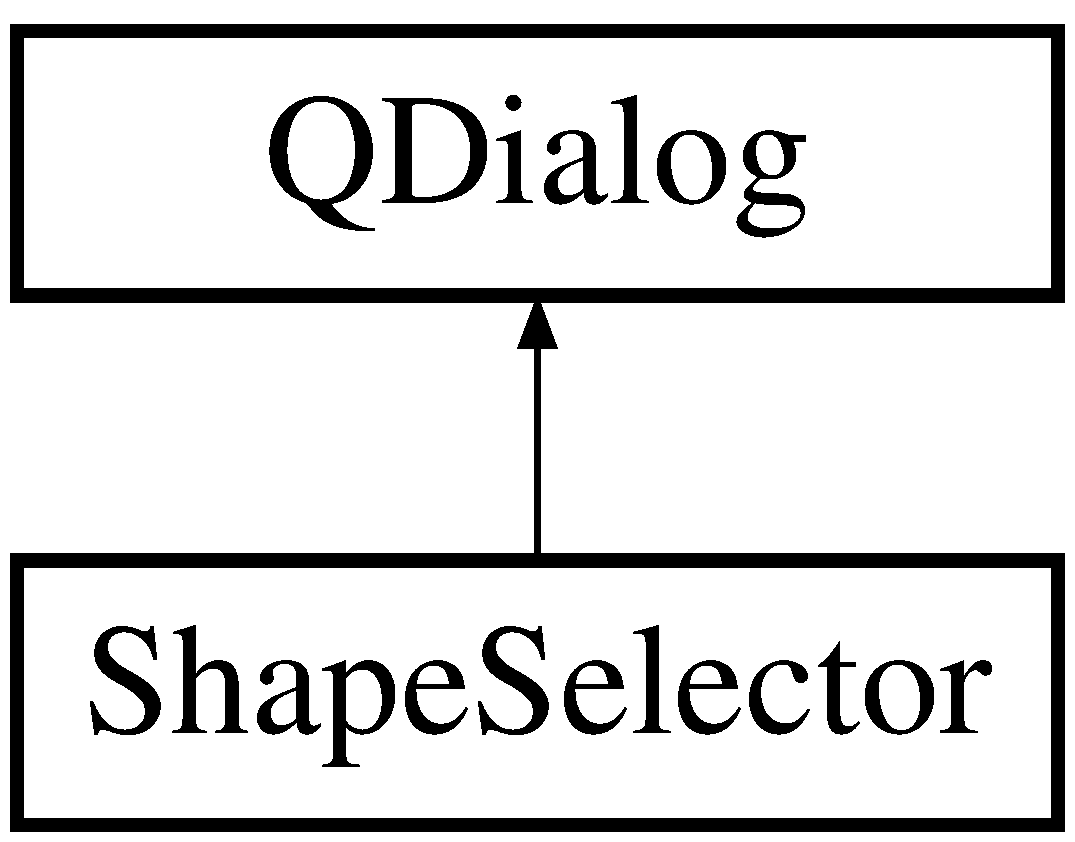
\includegraphics[height=2.000000cm]{class_shape_selector}
\end{center}
\end{figure}
\subsection*{Signals}
\begin{DoxyCompactItemize}
\item 
void \hyperlink{class_shape_selector_acf6369f1e2033024e8d507ab57e0d837}{packing\+Accepted} (\hyperlink{class_packing}{Packing} $\ast$p)
\end{DoxyCompactItemize}
\subsection*{Public Member Functions}
\begin{DoxyCompactItemize}
\item 
\hyperlink{class_shape_selector_ad74aca0ebd306645e05076f4624e1ab1}{Shape\+Selector} (Q\+Widget $\ast$parent=0)
\item 
\hyperlink{class_shape_selector_a206577c05a50a137e3f69022b75bcc4d}{$\sim$\+Shape\+Selector} ()
\end{DoxyCompactItemize}


\subsection{Constructor \& Destructor Documentation}
\hypertarget{class_shape_selector_ad74aca0ebd306645e05076f4624e1ab1}{}\index{Shape\+Selector@{Shape\+Selector}!Shape\+Selector@{Shape\+Selector}}
\index{Shape\+Selector@{Shape\+Selector}!Shape\+Selector@{Shape\+Selector}}
\subsubsection[{Shape\+Selector(\+Q\+Widget $\ast$parent=0)}]{\setlength{\rightskip}{0pt plus 5cm}Shape\+Selector\+::\+Shape\+Selector (
\begin{DoxyParamCaption}
\item[{Q\+Widget $\ast$}]{parent = {\ttfamily 0}}
\end{DoxyParamCaption}
)\hspace{0.3cm}{\ttfamily [explicit]}}\label{class_shape_selector_ad74aca0ebd306645e05076f4624e1ab1}
\hypertarget{class_shape_selector_a206577c05a50a137e3f69022b75bcc4d}{}\index{Shape\+Selector@{Shape\+Selector}!````~Shape\+Selector@{$\sim$\+Shape\+Selector}}
\index{````~Shape\+Selector@{$\sim$\+Shape\+Selector}!Shape\+Selector@{Shape\+Selector}}
\subsubsection[{$\sim$\+Shape\+Selector()}]{\setlength{\rightskip}{0pt plus 5cm}Shape\+Selector\+::$\sim$\+Shape\+Selector (
\begin{DoxyParamCaption}
{}
\end{DoxyParamCaption}
)}\label{class_shape_selector_a206577c05a50a137e3f69022b75bcc4d}


\subsection{Member Function Documentation}
\hypertarget{class_shape_selector_acf6369f1e2033024e8d507ab57e0d837}{}\index{Shape\+Selector@{Shape\+Selector}!packing\+Accepted@{packing\+Accepted}}
\index{packing\+Accepted@{packing\+Accepted}!Shape\+Selector@{Shape\+Selector}}
\subsubsection[{packing\+Accepted}]{\setlength{\rightskip}{0pt plus 5cm}void Shape\+Selector\+::packing\+Accepted (
\begin{DoxyParamCaption}
\item[{{\bf Packing} $\ast$}]{p}
\end{DoxyParamCaption}
)\hspace{0.3cm}{\ttfamily [signal]}}\label{class_shape_selector_acf6369f1e2033024e8d507ab57e0d837}


The documentation for this class was generated from the following files\+:\begin{DoxyCompactItemize}
\item 
ui/\hyperlink{_shape_selector_8hpp}{Shape\+Selector.\+hpp}\item 
ui/\hyperlink{_shape_selector_8cpp}{Shape\+Selector.\+cpp}\end{DoxyCompactItemize}

\hypertarget{class_shape_selector_graphics_view}{}\section{Shape\+Selector\+Graphics\+View Class Reference}
\label{class_shape_selector_graphics_view}\index{Shape\+Selector\+Graphics\+View@{Shape\+Selector\+Graphics\+View}}


{\ttfamily \#include $<$Shape\+Selector\+Graphics\+View.\+hpp$>$}

Inheritance diagram for Shape\+Selector\+Graphics\+View\+:\begin{figure}[H]
\begin{center}
\leavevmode
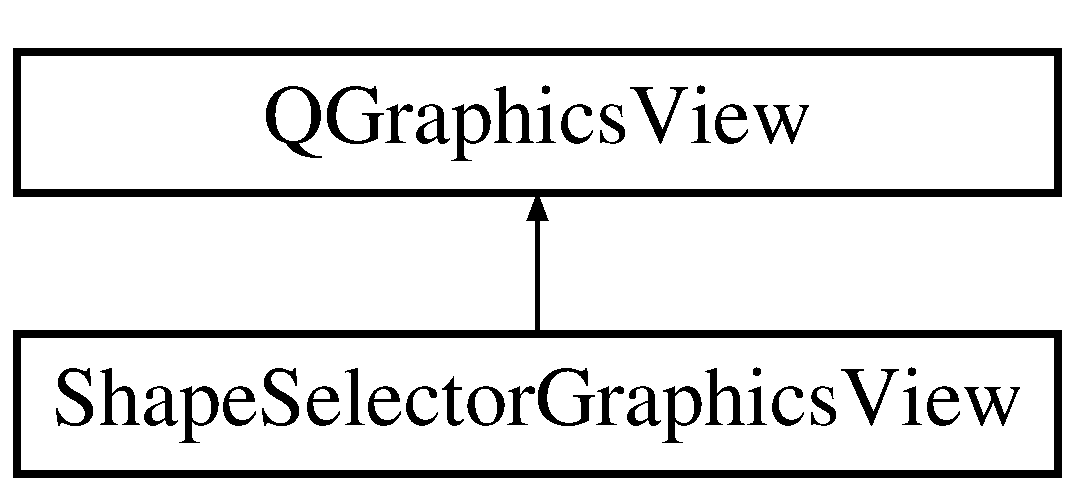
\includegraphics[height=2.000000cm]{class_shape_selector_graphics_view}
\end{center}
\end{figure}
\subsection*{Signals}
\begin{DoxyCompactItemize}
\item 
void \hyperlink{class_shape_selector_graphics_view_ad071a85e73af645061bf1ea8007707b6}{got\+Click} (Q\+Point\+F scenepos)
\end{DoxyCompactItemize}
\subsection*{Public Member Functions}
\begin{DoxyCompactItemize}
\item 
\hyperlink{class_shape_selector_graphics_view_addc27cb99f515e97fb1c9dfd577ccda0}{Shape\+Selector\+Graphics\+View} (Q\+Widget $\ast$parent=nullptr)
\item 
\hyperlink{class_shape_selector_graphics_view_a5ed676b4b4215698bdff8c7959ec55d7}{Shape\+Selector\+Graphics\+View} (Q\+Graphics\+Scene $\ast$scene, Q\+Widget $\ast$parent=nullptr)
\item 
virtual int \hyperlink{class_shape_selector_graphics_view_aa2aa9700ee783cb4140b709ac4d72378}{height\+For\+Width} (int w) const 
\item 
virtual bool \hyperlink{class_shape_selector_graphics_view_a95354b0f1d0f40c7089d9ab7c07ff51f}{has\+Height\+For\+Width} () const 
\end{DoxyCompactItemize}
\subsection*{Protected Member Functions}
\begin{DoxyCompactItemize}
\item 
virtual void \hyperlink{class_shape_selector_graphics_view_a7b9025eca69525d8486c5733fc44b0b0}{resize\+Event} (Q\+Resize\+Event $\ast$event)
\item 
virtual void \hyperlink{class_shape_selector_graphics_view_aae96cfbbb5fd87e8cbca3e3a407fb769}{mouse\+Press\+Event} (Q\+Mouse\+Event $\ast$event)
\end{DoxyCompactItemize}


\subsection{Constructor \& Destructor Documentation}
\hypertarget{class_shape_selector_graphics_view_addc27cb99f515e97fb1c9dfd577ccda0}{}\index{Shape\+Selector\+Graphics\+View@{Shape\+Selector\+Graphics\+View}!Shape\+Selector\+Graphics\+View@{Shape\+Selector\+Graphics\+View}}
\index{Shape\+Selector\+Graphics\+View@{Shape\+Selector\+Graphics\+View}!Shape\+Selector\+Graphics\+View@{Shape\+Selector\+Graphics\+View}}
\subsubsection[{Shape\+Selector\+Graphics\+View(\+Q\+Widget $\ast$parent=nullptr)}]{\setlength{\rightskip}{0pt plus 5cm}Shape\+Selector\+Graphics\+View\+::\+Shape\+Selector\+Graphics\+View (
\begin{DoxyParamCaption}
\item[{Q\+Widget $\ast$}]{parent = {\ttfamily nullptr}}
\end{DoxyParamCaption}
)}\label{class_shape_selector_graphics_view_addc27cb99f515e97fb1c9dfd577ccda0}
\hypertarget{class_shape_selector_graphics_view_a5ed676b4b4215698bdff8c7959ec55d7}{}\index{Shape\+Selector\+Graphics\+View@{Shape\+Selector\+Graphics\+View}!Shape\+Selector\+Graphics\+View@{Shape\+Selector\+Graphics\+View}}
\index{Shape\+Selector\+Graphics\+View@{Shape\+Selector\+Graphics\+View}!Shape\+Selector\+Graphics\+View@{Shape\+Selector\+Graphics\+View}}
\subsubsection[{Shape\+Selector\+Graphics\+View(\+Q\+Graphics\+Scene $\ast$scene, Q\+Widget $\ast$parent=nullptr)}]{\setlength{\rightskip}{0pt plus 5cm}Shape\+Selector\+Graphics\+View\+::\+Shape\+Selector\+Graphics\+View (
\begin{DoxyParamCaption}
\item[{Q\+Graphics\+Scene $\ast$}]{scene, }
\item[{Q\+Widget $\ast$}]{parent = {\ttfamily nullptr}}
\end{DoxyParamCaption}
)}\label{class_shape_selector_graphics_view_a5ed676b4b4215698bdff8c7959ec55d7}


\subsection{Member Function Documentation}
\hypertarget{class_shape_selector_graphics_view_ad071a85e73af645061bf1ea8007707b6}{}\index{Shape\+Selector\+Graphics\+View@{Shape\+Selector\+Graphics\+View}!got\+Click@{got\+Click}}
\index{got\+Click@{got\+Click}!Shape\+Selector\+Graphics\+View@{Shape\+Selector\+Graphics\+View}}
\subsubsection[{got\+Click}]{\setlength{\rightskip}{0pt plus 5cm}void Shape\+Selector\+Graphics\+View\+::got\+Click (
\begin{DoxyParamCaption}
\item[{Q\+Point\+F}]{scenepos}
\end{DoxyParamCaption}
)\hspace{0.3cm}{\ttfamily [signal]}}\label{class_shape_selector_graphics_view_ad071a85e73af645061bf1ea8007707b6}
\hypertarget{class_shape_selector_graphics_view_a95354b0f1d0f40c7089d9ab7c07ff51f}{}\index{Shape\+Selector\+Graphics\+View@{Shape\+Selector\+Graphics\+View}!has\+Height\+For\+Width@{has\+Height\+For\+Width}}
\index{has\+Height\+For\+Width@{has\+Height\+For\+Width}!Shape\+Selector\+Graphics\+View@{Shape\+Selector\+Graphics\+View}}
\subsubsection[{has\+Height\+For\+Width() const }]{\setlength{\rightskip}{0pt plus 5cm}virtual bool Shape\+Selector\+Graphics\+View\+::has\+Height\+For\+Width (
\begin{DoxyParamCaption}
{}
\end{DoxyParamCaption}
) const\hspace{0.3cm}{\ttfamily [inline]}, {\ttfamily [virtual]}}\label{class_shape_selector_graphics_view_a95354b0f1d0f40c7089d9ab7c07ff51f}
\hypertarget{class_shape_selector_graphics_view_aa2aa9700ee783cb4140b709ac4d72378}{}\index{Shape\+Selector\+Graphics\+View@{Shape\+Selector\+Graphics\+View}!height\+For\+Width@{height\+For\+Width}}
\index{height\+For\+Width@{height\+For\+Width}!Shape\+Selector\+Graphics\+View@{Shape\+Selector\+Graphics\+View}}
\subsubsection[{height\+For\+Width(int w) const }]{\setlength{\rightskip}{0pt plus 5cm}virtual int Shape\+Selector\+Graphics\+View\+::height\+For\+Width (
\begin{DoxyParamCaption}
\item[{int}]{w}
\end{DoxyParamCaption}
) const\hspace{0.3cm}{\ttfamily [inline]}, {\ttfamily [virtual]}}\label{class_shape_selector_graphics_view_aa2aa9700ee783cb4140b709ac4d72378}
\hypertarget{class_shape_selector_graphics_view_aae96cfbbb5fd87e8cbca3e3a407fb769}{}\index{Shape\+Selector\+Graphics\+View@{Shape\+Selector\+Graphics\+View}!mouse\+Press\+Event@{mouse\+Press\+Event}}
\index{mouse\+Press\+Event@{mouse\+Press\+Event}!Shape\+Selector\+Graphics\+View@{Shape\+Selector\+Graphics\+View}}
\subsubsection[{mouse\+Press\+Event(\+Q\+Mouse\+Event $\ast$event)}]{\setlength{\rightskip}{0pt plus 5cm}void Shape\+Selector\+Graphics\+View\+::mouse\+Press\+Event (
\begin{DoxyParamCaption}
\item[{Q\+Mouse\+Event $\ast$}]{event}
\end{DoxyParamCaption}
)\hspace{0.3cm}{\ttfamily [protected]}, {\ttfamily [virtual]}}\label{class_shape_selector_graphics_view_aae96cfbbb5fd87e8cbca3e3a407fb769}
\hypertarget{class_shape_selector_graphics_view_a7b9025eca69525d8486c5733fc44b0b0}{}\index{Shape\+Selector\+Graphics\+View@{Shape\+Selector\+Graphics\+View}!resize\+Event@{resize\+Event}}
\index{resize\+Event@{resize\+Event}!Shape\+Selector\+Graphics\+View@{Shape\+Selector\+Graphics\+View}}
\subsubsection[{resize\+Event(\+Q\+Resize\+Event $\ast$event)}]{\setlength{\rightskip}{0pt plus 5cm}void Shape\+Selector\+Graphics\+View\+::resize\+Event (
\begin{DoxyParamCaption}
\item[{Q\+Resize\+Event $\ast$}]{event}
\end{DoxyParamCaption}
)\hspace{0.3cm}{\ttfamily [protected]}, {\ttfamily [virtual]}}\label{class_shape_selector_graphics_view_a7b9025eca69525d8486c5733fc44b0b0}


The documentation for this class was generated from the following files\+:\begin{DoxyCompactItemize}
\item 
graphics/\hyperlink{_shape_selector_graphics_view_8hpp}{Shape\+Selector\+Graphics\+View.\+hpp}\item 
graphics/\hyperlink{_shape_selector_graphics_view_8cpp}{Shape\+Selector\+Graphics\+View.\+cpp}\end{DoxyCompactItemize}

\chapter{File Documentation}
\hypertarget{_edge_8cpp}{}\section{graph/\+Edge.cpp File Reference}
\label{_edge_8cpp}\index{graph/\+Edge.\+cpp@{graph/\+Edge.\+cpp}}
{\ttfamily \#include \char`\"{}Edge.\+hpp\char`\"{}}\\*

\hypertarget{_edge_8hpp}{}\section{graph/\+Edge.hpp File Reference}
\label{_edge_8hpp}\index{graph/\+Edge.\+hpp@{graph/\+Edge.\+hpp}}
\subsection*{Classes}
\begin{DoxyCompactItemize}
\item 
class \hyperlink{class_circles_1_1_graph_1_1_edge}{Circles\+::\+Graph\+::\+Edge}
\end{DoxyCompactItemize}
\subsection*{Namespaces}
\begin{DoxyCompactItemize}
\item 
 \hyperlink{namespace_circles}{Circles}
\item 
 \hyperlink{namespace_circles_1_1_graph}{Circles\+::\+Graph}
\end{DoxyCompactItemize}
\subsection*{Functions}
\begin{DoxyCompactItemize}
\item 
bool \hyperlink{namespace_circles_1_1_graph_a77922e41074a56d81cb1f75767b6b013}{Circles\+::\+Graph\+::operator==} (const \hyperlink{class_circles_1_1_graph_1_1_edge}{Edge} \&lhs, const \hyperlink{class_circles_1_1_graph_1_1_edge}{Edge} \&rhs)
\end{DoxyCompactItemize}

\hypertarget{_graph_8cpp}{}\section{graph/\+Graph.cpp File Reference}
\label{_graph_8cpp}\index{graph/\+Graph.\+cpp@{graph/\+Graph.\+cpp}}
{\ttfamily \#include \char`\"{}Graph.\+hpp\char`\"{}}\\*

\hypertarget{_graph_8hpp}{}\section{graph/\+Graph.hpp File Reference}
\label{_graph_8hpp}\index{graph/\+Graph.\+hpp@{graph/\+Graph.\+hpp}}
{\ttfamily \#include $<$Q\+Hash$>$}\\*
{\ttfamily \#include $<$Q\+Set$>$}\\*
{\ttfamily \#include $<$Q\+List$>$}\\*
{\ttfamily \#include $<$memory$>$}\\*
{\ttfamily \#include $<$graph/\+Edge.\+hpp$>$}\\*
\subsection*{Classes}
\begin{DoxyCompactItemize}
\item 
class \hyperlink{class_circles_1_1_graph_1_1_graph}{Circles\+::\+Graph\+::\+Graph}
\end{DoxyCompactItemize}
\subsection*{Namespaces}
\begin{DoxyCompactItemize}
\item 
 \hyperlink{namespace_circles}{Circles}
\item 
 \hyperlink{namespace_circles_1_1_graph}{Circles\+::\+Graph}
\end{DoxyCompactItemize}
\subsection*{Typedefs}
\begin{DoxyCompactItemize}
\item 
typedef int \hyperlink{namespace_circles_1_1_graph_afab3817d1ee8e2074e82866c27a1058b}{Circles\+::\+Graph\+::\+Node}
\end{DoxyCompactItemize}

\hypertarget{_boundary_8cpp}{}\section{graphics/\+Boundary.cpp File Reference}
\label{_boundary_8cpp}\index{graphics/\+Boundary.\+cpp@{graphics/\+Boundary.\+cpp}}
{\ttfamily \#include \char`\"{}Boundary.\+hpp\char`\"{}}\\*
{\ttfamily \#include \char`\"{}Qt\+Widgets\char`\"{}}\\*
{\ttfamily \#include $<$cmath$>$}\\*
\subsection*{Macros}
\begin{DoxyCompactItemize}
\item 
\#define \hyperlink{_boundary_8cpp_a598a3330b3c21701223ee0ca14316eca}{P\+I}~3.\+141592654
\end{DoxyCompactItemize}


\subsection{Macro Definition Documentation}
\hypertarget{_boundary_8cpp_a598a3330b3c21701223ee0ca14316eca}{}\index{Boundary.\+cpp@{Boundary.\+cpp}!P\+I@{P\+I}}
\index{P\+I@{P\+I}!Boundary.\+cpp@{Boundary.\+cpp}}
\subsubsection[{P\+I}]{\setlength{\rightskip}{0pt plus 5cm}\#define P\+I~3.\+141592654}\label{_boundary_8cpp_a598a3330b3c21701223ee0ca14316eca}

\hypertarget{_boundary_8hpp}{}\section{graphics/\+Boundary.hpp File Reference}
\label{_boundary_8hpp}\index{graphics/\+Boundary.\+hpp@{graphics/\+Boundary.\+hpp}}
{\ttfamily \#include $<$Q\+Widget$>$}\\*
{\ttfamily \#include $<$Q\+Graphics\+Item$>$}\\*
\subsection*{Classes}
\begin{DoxyCompactItemize}
\item 
class \hyperlink{class_boundary}{Boundary}
\end{DoxyCompactItemize}

\hypertarget{graphics_2_circle_8cpp}{}\section{graphics/\+Circle.cpp File Reference}
\label{graphics_2_circle_8cpp}\index{graphics/\+Circle.\+cpp@{graphics/\+Circle.\+cpp}}
{\ttfamily \#include \char`\"{}Circle.\+hpp\char`\"{}}\\*
{\ttfamily \#include $<$cmath$>$}\\*
{\ttfamily \#include $<$Qt\+Widgets$>$}\\*
{\ttfamily \#include $<$Q\+Painter\+Path$>$}\\*
{\ttfamily \#include \char`\"{}Packing.\+hpp\char`\"{}}\\*

\hypertarget{packing_2_circle_8cpp}{}\section{packing/\+Circle.cpp File Reference}
\label{packing_2_circle_8cpp}\index{packing/\+Circle.\+cpp@{packing/\+Circle.\+cpp}}
{\ttfamily \#include \char`\"{}Circle.\+hpp\char`\"{}}\\*

\hypertarget{graphics_2_circle_8hpp}{}\section{graphics/\+Circle.hpp File Reference}
\label{graphics_2_circle_8hpp}\index{graphics/\+Circle.\+hpp@{graphics/\+Circle.\+hpp}}
{\ttfamily \#include $<$Q\+Graphics\+Item$>$}\\*
{\ttfamily \#include $<$Q\+Widget$>$}\\*
{\ttfamily \#include $<$Q\+Painter\+Path$>$}\\*
{\ttfamily \#include \char`\"{}../\+Node.\+hpp\char`\"{}}\\*
{\ttfamily \#include \char`\"{}Packing.\+hpp\char`\"{}}\\*
\subsection*{Classes}
\begin{DoxyCompactItemize}
\item 
class \hyperlink{class_circle}{Circle}
\begin{DoxyCompactList}\small\item\em The \hyperlink{class_circle}{Circle} class represents an abstract circle. A circle may exist in either a hyperbolic or euclidean geometry. \end{DoxyCompactList}\end{DoxyCompactItemize}

\hypertarget{packing_2_circle_8hpp}{}\section{packing/\+Circle.hpp File Reference}
\label{packing_2_circle_8hpp}\index{packing/\+Circle.\+hpp@{packing/\+Circle.\+hpp}}
{\ttfamily \#include $<$Q\+Point\+F$>$}\\*
\subsection*{Classes}
\begin{DoxyCompactItemize}
\item 
class \hyperlink{class_circles_1_1_packing_1_1_circle}{Circles\+::\+Packing\+::\+Circle}
\end{DoxyCompactItemize}
\subsection*{Namespaces}
\begin{DoxyCompactItemize}
\item 
 \hyperlink{namespace_circles}{Circles}
\item 
 \hyperlink{namespace_circles_1_1_packing}{Circles\+::\+Packing}
\end{DoxyCompactItemize}
\subsection*{Functions}
\begin{DoxyCompactItemize}
\item 
bool \hyperlink{namespace_circles_1_1_packing_a372a7d94ba42f1b7ce411fd596a29710}{Circles\+::\+Packing\+::operator$<$} (const \hyperlink{class_circles_1_1_packing_1_1_circle}{Circle} \&lhs, const \hyperlink{class_circles_1_1_packing_1_1_circle}{Circle} \&rhs)
\end{DoxyCompactItemize}

\hypertarget{_connector_8cpp}{}\section{graphics/\+Connector.cpp File Reference}
\label{_connector_8cpp}\index{graphics/\+Connector.\+cpp@{graphics/\+Connector.\+cpp}}
{\ttfamily \#include \char`\"{}Connector.\+hpp\char`\"{}}\\*
{\ttfamily \#include $<$cmath$>$}\\*
{\ttfamily \#include $<$Qt\+Widgets$>$}\\*

\hypertarget{_connector_8hpp}{}\section{graphics/\+Connector.hpp File Reference}
\label{_connector_8hpp}\index{graphics/\+Connector.\+hpp@{graphics/\+Connector.\+hpp}}
{\ttfamily \#include $<$Q\+Widget$>$}\\*
{\ttfamily \#include $<$Q\+Graphics\+Item$>$}\\*
{\ttfamily \#include \char`\"{}../\+Node.\+hpp\char`\"{}}\\*
\subsection*{Classes}
\begin{DoxyCompactItemize}
\item 
class \hyperlink{class_connector}{Connector}
\end{DoxyCompactItemize}

\hypertarget{graphics_2_packing_8cpp}{}\section{graphics/\+Packing.cpp File Reference}
\label{graphics_2_packing_8cpp}\index{graphics/\+Packing.\+cpp@{graphics/\+Packing.\+cpp}}
{\ttfamily \#include \char`\"{}Packing.\+hpp\char`\"{}}\\*
{\ttfamily \#include $<$cmath$>$}\\*
{\ttfamily \#include $<$complex$>$}\\*
{\ttfamily \#include $<$Q\+Widget$>$}\\*
{\ttfamily \#include $<$Q\+Debug$>$}\\*
{\ttfamily \#include \char`\"{}Boundary.\+hpp\char`\"{}}\\*
\subsection*{Macros}
\begin{DoxyCompactItemize}
\item 
\#define \hyperlink{graphics_2_packing_8cpp_a598a3330b3c21701223ee0ca14316eca}{P\+I}~3.\+1415926535897932384626433
\end{DoxyCompactItemize}


\subsection{Macro Definition Documentation}
\hypertarget{graphics_2_packing_8cpp_a598a3330b3c21701223ee0ca14316eca}{}\index{graphics/\+Packing.\+cpp@{graphics/\+Packing.\+cpp}!P\+I@{P\+I}}
\index{P\+I@{P\+I}!graphics/\+Packing.\+cpp@{graphics/\+Packing.\+cpp}}
\subsubsection[{P\+I}]{\setlength{\rightskip}{0pt plus 5cm}\#define P\+I~3.\+1415926535897932384626433}\label{graphics_2_packing_8cpp_a598a3330b3c21701223ee0ca14316eca}

\hypertarget{packing_2_packing_8cpp}{}\section{packing/\+Packing.cpp File Reference}
\label{packing_2_packing_8cpp}\index{packing/\+Packing.\+cpp@{packing/\+Packing.\+cpp}}
{\ttfamily \#include $<$algorithm$>$}\\*
{\ttfamily \#include \char`\"{}Packing.\+hpp\char`\"{}}\\*

\hypertarget{graphics_2_packing_8hpp}{}\section{graphics/\+Packing.hpp File Reference}
\label{graphics_2_packing_8hpp}\index{graphics/\+Packing.\+hpp@{graphics/\+Packing.\+hpp}}
{\ttfamily \#include $<$Q\+Graphics\+Scene$>$}\\*
{\ttfamily \#include $<$Q\+Graphics\+Scene\+Mouse\+Event$>$}\\*
{\ttfamily \#include $<$Q\+Widget$>$}\\*
{\ttfamily \#include $<$Q\+Object$>$}\\*
{\ttfamily \#include \char`\"{}../\+Node.\+hpp\char`\"{}}\\*
{\ttfamily \#include \char`\"{}Circle.\+hpp\char`\"{}}\\*
{\ttfamily \#include \char`\"{}Connector.\+hpp\char`\"{}}\\*
{\ttfamily \#include \char`\"{}Boundary.\+hpp\char`\"{}}\\*
\subsection*{Classes}
\begin{DoxyCompactItemize}
\item 
class \hyperlink{class_packing}{Packing}
\begin{DoxyCompactList}\small\item\em The \hyperlink{class_packing}{Packing} class is an abstract class which defines a circle packing. A circle packing may be either euclidean or hyperbolic, as found in Euclidean\+Packing and Hyperbolic\+Packing. \end{DoxyCompactList}\end{DoxyCompactItemize}
\subsection*{Enumerations}
\begin{DoxyCompactItemize}
\item 
enum \hyperlink{graphics_2_packing_8hpp_a331874350131c9e1039dac50b427f8b9}{Packing\+Type} \{ \hyperlink{graphics_2_packing_8hpp_a331874350131c9e1039dac50b427f8b9aa4066bbe6791ed6bbfe12f55a60ed152}{Packing\+Type\+::\+Euclidean\+Packing}, 
\hyperlink{graphics_2_packing_8hpp_a331874350131c9e1039dac50b427f8b9af44d305ffa405b64040c7d4bc16953f9}{Packing\+Type\+::\+Hyperbolic\+Packing}
 \}\begin{DoxyCompactList}\small\item\em The Packing\+Type enum defines the geometries available to a \hyperlink{class_packing}{Packing}. A packing may either be euclidean, on the cartesian plane, or hyperbolic, on the poincare disc. \end{DoxyCompactList}
\end{DoxyCompactItemize}


\subsection{Enumeration Type Documentation}
\hypertarget{graphics_2_packing_8hpp_a331874350131c9e1039dac50b427f8b9}{}\index{graphics/\+Packing.\+hpp@{graphics/\+Packing.\+hpp}!Packing\+Type@{Packing\+Type}}
\index{Packing\+Type@{Packing\+Type}!graphics/\+Packing.\+hpp@{graphics/\+Packing.\+hpp}}
\subsubsection[{Packing\+Type}]{\setlength{\rightskip}{0pt plus 5cm}enum {\bf Packing\+Type}\hspace{0.3cm}{\ttfamily [strong]}}\label{graphics_2_packing_8hpp_a331874350131c9e1039dac50b427f8b9}


The Packing\+Type enum defines the geometries available to a \hyperlink{class_packing}{Packing}. A packing may either be euclidean, on the cartesian plane, or hyperbolic, on the poincare disc. 

\begin{Desc}
\item[Enumerator]\par
\begin{description}
\index{Euclidean\+Packing@{Euclidean\+Packing}!graphics/\+Packing.\+hpp@{graphics/\+Packing.\+hpp}}\index{graphics/\+Packing.\+hpp@{graphics/\+Packing.\+hpp}!Euclidean\+Packing@{Euclidean\+Packing}}\item[{\em 
\hypertarget{graphics_2_packing_8hpp_a331874350131c9e1039dac50b427f8b9aa4066bbe6791ed6bbfe12f55a60ed152}{}Euclidean\+Packing\label{graphics_2_packing_8hpp_a331874350131c9e1039dac50b427f8b9aa4066bbe6791ed6bbfe12f55a60ed152}
}]\index{Hyperbolic\+Packing@{Hyperbolic\+Packing}!graphics/\+Packing.\+hpp@{graphics/\+Packing.\+hpp}}\index{graphics/\+Packing.\+hpp@{graphics/\+Packing.\+hpp}!Hyperbolic\+Packing@{Hyperbolic\+Packing}}\item[{\em 
\hypertarget{graphics_2_packing_8hpp_a331874350131c9e1039dac50b427f8b9af44d305ffa405b64040c7d4bc16953f9}{}Hyperbolic\+Packing\label{graphics_2_packing_8hpp_a331874350131c9e1039dac50b427f8b9af44d305ffa405b64040c7d4bc16953f9}
}]\end{description}
\end{Desc}

\hypertarget{packing_2_packing_8hpp}{}\section{packing/\+Packing.hpp File Reference}
\label{packing_2_packing_8hpp}\index{packing/\+Packing.\+hpp@{packing/\+Packing.\+hpp}}
{\ttfamily \#include $<$memory$>$}\\*
{\ttfamily \#include $<$Q\+List$>$}\\*
{\ttfamily \#include $<$Q\+Map$>$}\\*
{\ttfamily \#include $<$graph/\+Graph.\+hpp$>$}\\*
{\ttfamily \#include $<$packing/\+Circle.\+hpp$>$}\\*
\subsection*{Classes}
\begin{DoxyCompactItemize}
\item 
class \hyperlink{class_circles_1_1_packing_1_1_packing}{Circles\+::\+Packing\+::\+Packing}
\end{DoxyCompactItemize}
\subsection*{Namespaces}
\begin{DoxyCompactItemize}
\item 
 \hyperlink{namespace_circles}{Circles}
\item 
 \hyperlink{namespace_circles_1_1_packing}{Circles\+::\+Packing}
\end{DoxyCompactItemize}

\hypertarget{_selection_packing_8cpp}{}\section{graphics/\+Selection\+Packing.cpp File Reference}
\label{_selection_packing_8cpp}\index{graphics/\+Selection\+Packing.\+cpp@{graphics/\+Selection\+Packing.\+cpp}}
{\ttfamily \#include \char`\"{}Selection\+Packing.\+hpp\char`\"{}}\\*
{\ttfamily \#include $<$typeinfo$>$}\\*
{\ttfamily \#include $<$Q\+Debug$>$}\\*

\hypertarget{_selection_packing_8hpp}{}\section{graphics/\+Selection\+Packing.hpp File Reference}
\label{_selection_packing_8hpp}\index{graphics/\+Selection\+Packing.\+hpp@{graphics/\+Selection\+Packing.\+hpp}}
{\ttfamily \#include $<$Q\+Widget$>$}\\*
{\ttfamily \#include $<$Q\+Graphics\+Scene$>$}\\*
{\ttfamily \#include $<$Q\+Graphics\+Scene\+Mouse\+Event$>$}\\*
{\ttfamily \#include \char`\"{}Packing.\+hpp\char`\"{}}\\*
{\ttfamily \#include \char`\"{}Circle.\+hpp\char`\"{}}\\*
\subsection*{Classes}
\begin{DoxyCompactItemize}
\item 
class \hyperlink{class_selection_packing}{Selection\+Packing}
\end{DoxyCompactItemize}

\hypertarget{_selection_vertex_8cpp}{}\section{graphics/\+Selection\+Vertex.cpp File Reference}
\label{_selection_vertex_8cpp}\index{graphics/\+Selection\+Vertex.\+cpp@{graphics/\+Selection\+Vertex.\+cpp}}
{\ttfamily \#include \char`\"{}Selection\+Vertex.\+hpp\char`\"{}}\\*
{\ttfamily \#include $<$Q\+Painter$>$}\\*
{\ttfamily \#include $<$Q\+Debug$>$}\\*
{\ttfamily \#include $<$Q\+Style\+Option\+Graphics\+Item$>$}\\*

\hypertarget{_selection_vertex_8hpp}{}\section{graphics/\+Selection\+Vertex.hpp File Reference}
\label{_selection_vertex_8hpp}\index{graphics/\+Selection\+Vertex.\+hpp@{graphics/\+Selection\+Vertex.\+hpp}}
{\ttfamily \#include $<$Q\+Object$>$}\\*
{\ttfamily \#include $<$Q\+Widget$>$}\\*
{\ttfamily \#include $<$Q\+Graphics\+Item$>$}\\*
\subsection*{Classes}
\begin{DoxyCompactItemize}
\item 
class \hyperlink{class_selection_vertex}{Selection\+Vertex}
\end{DoxyCompactItemize}

\hypertarget{_shape_selector_graphics_view_8cpp}{}\section{graphics/\+Shape\+Selector\+Graphics\+View.cpp File Reference}
\label{_shape_selector_graphics_view_8cpp}\index{graphics/\+Shape\+Selector\+Graphics\+View.\+cpp@{graphics/\+Shape\+Selector\+Graphics\+View.\+cpp}}
{\ttfamily \#include \char`\"{}Shape\+Selector\+Graphics\+View.\+hpp\char`\"{}}\\*
{\ttfamily \#include $<$Q\+Resize\+Event$>$}\\*

\hypertarget{_shape_selector_graphics_view_8hpp}{}\section{graphics/\+Shape\+Selector\+Graphics\+View.hpp File Reference}
\label{_shape_selector_graphics_view_8hpp}\index{graphics/\+Shape\+Selector\+Graphics\+View.\+hpp@{graphics/\+Shape\+Selector\+Graphics\+View.\+hpp}}
{\ttfamily \#include $<$Q\+Object$>$}\\*
{\ttfamily \#include $<$Q\+Widget$>$}\\*
{\ttfamily \#include $<$Q\+Graphics\+Scene$>$}\\*
{\ttfamily \#include $<$Q\+Graphics\+View$>$}\\*
{\ttfamily \#include $<$Q\+Point\+F$>$}\\*
\subsection*{Classes}
\begin{DoxyCompactItemize}
\item 
class \hyperlink{class_shape_selector_graphics_view}{Shape\+Selector\+Graphics\+View}
\end{DoxyCompactItemize}

\hypertarget{main_8cpp}{}\section{main.\+cpp File Reference}
\label{main_8cpp}\index{main.\+cpp@{main.\+cpp}}
{\ttfamily \#include \char`\"{}ui/\+Main\+Window.\+hpp\char`\"{}}\\*
{\ttfamily \#include $<$Q\+Application$>$}\\*
\subsection*{Functions}
\begin{DoxyCompactItemize}
\item 
int \hyperlink{main_8cpp_a0ddf1224851353fc92bfbff6f499fa97}{main} (int argc, char $\ast$argv\mbox{[}$\,$\mbox{]})
\end{DoxyCompactItemize}


\subsection{Function Documentation}
\hypertarget{main_8cpp_a0ddf1224851353fc92bfbff6f499fa97}{}\index{main.\+cpp@{main.\+cpp}!main@{main}}
\index{main@{main}!main.\+cpp@{main.\+cpp}}
\subsubsection[{main(int argc, char $\ast$argv[])}]{\setlength{\rightskip}{0pt plus 5cm}int main (
\begin{DoxyParamCaption}
\item[{int}]{argc, }
\item[{char $\ast$}]{argv\mbox{[}$\,$\mbox{]}}
\end{DoxyParamCaption}
)}\label{main_8cpp_a0ddf1224851353fc92bfbff6f499fa97}

\hypertarget{_node_8cpp}{}\section{Node.\+cpp File Reference}
\label{_node_8cpp}\index{Node.\+cpp@{Node.\+cpp}}
{\ttfamily \#include \char`\"{}Node.\+hpp\char`\"{}}\\*
{\ttfamily \#include $<$cmath$>$}\\*
\subsection*{Macros}
\begin{DoxyCompactItemize}
\item 
\#define \hyperlink{_node_8cpp_a598a3330b3c21701223ee0ca14316eca}{P\+I}~3.\+1415926535897932384626433
\end{DoxyCompactItemize}


\subsection{Macro Definition Documentation}
\hypertarget{_node_8cpp_a598a3330b3c21701223ee0ca14316eca}{}\index{Node.\+cpp@{Node.\+cpp}!P\+I@{P\+I}}
\index{P\+I@{P\+I}!Node.\+cpp@{Node.\+cpp}}
\subsubsection[{P\+I}]{\setlength{\rightskip}{0pt plus 5cm}\#define P\+I~3.\+1415926535897932384626433}\label{_node_8cpp_a598a3330b3c21701223ee0ca14316eca}

\hypertarget{_node_8hpp}{}\section{Node.\+hpp File Reference}
\label{_node_8hpp}\index{Node.\+hpp@{Node.\+hpp}}
{\ttfamily \#include $<$Q\+Widget$>$}\\*
\subsection*{Classes}
\begin{DoxyCompactItemize}
\item 
class \hyperlink{class_node}{Node}
\begin{DoxyCompactList}\small\item\em The \hyperlink{class_node}{Node} class represents the metadata of a circle in a circle packing. \end{DoxyCompactList}\end{DoxyCompactItemize}

\hypertarget{_euclid_circle_8cpp}{}\section{packing/\+Euclid\+Circle.cpp File Reference}
\label{_euclid_circle_8cpp}\index{packing/\+Euclid\+Circle.\+cpp@{packing/\+Euclid\+Circle.\+cpp}}
{\ttfamily \#include \char`\"{}Euclid\+Circle.\+hpp\char`\"{}}\\*

\hypertarget{_euclid_circle_8hpp}{}\section{packing/\+Euclid\+Circle.hpp File Reference}
\label{_euclid_circle_8hpp}\index{packing/\+Euclid\+Circle.\+hpp@{packing/\+Euclid\+Circle.\+hpp}}
{\ttfamily \#include $<$packing/\+Circle.\+hpp$>$}\\*
\subsection*{Classes}
\begin{DoxyCompactItemize}
\item 
class \hyperlink{class_circles_1_1_packing_1_1_euclid_circle}{Circles\+::\+Packing\+::\+Euclid\+Circle}
\end{DoxyCompactItemize}
\subsection*{Namespaces}
\begin{DoxyCompactItemize}
\item 
 \hyperlink{namespace_circles}{Circles}
\item 
 \hyperlink{namespace_circles_1_1_packing}{Circles\+::\+Packing}
\end{DoxyCompactItemize}
\subsection*{Functions}
\begin{DoxyCompactItemize}
\item 
bool \hyperlink{namespace_circles_1_1_packing_a2fcf53805f473b2c72013862fb4d87e5}{Circles\+::\+Packing\+::operator==} (const \hyperlink{class_circles_1_1_packing_1_1_euclid_circle}{Euclid\+Circle} \&lhs, const \hyperlink{class_circles_1_1_packing_1_1_euclid_circle}{Euclid\+Circle} \&rhs)
\end{DoxyCompactItemize}

\hypertarget{_euclid_packing_8cpp}{}\section{packing/\+Euclid\+Packing.cpp File Reference}
\label{_euclid_packing_8cpp}\index{packing/\+Euclid\+Packing.\+cpp@{packing/\+Euclid\+Packing.\+cpp}}
{\ttfamily \#include \char`\"{}Euclid\+Packing.\+hpp\char`\"{}}\\*

\hypertarget{_euclid_packing_8hpp}{}\section{packing/\+Euclid\+Packing.hpp File Reference}
\label{_euclid_packing_8hpp}\index{packing/\+Euclid\+Packing.\+hpp@{packing/\+Euclid\+Packing.\+hpp}}
{\ttfamily \#include $<$Q\+Hash$>$}\\*
{\ttfamily \#include $<$memory$>$}\\*
{\ttfamily \#include \char`\"{}graph/\+Graph.\+hpp\char`\"{}}\\*
{\ttfamily \#include \char`\"{}packing/\+Packing.\+hpp\char`\"{}}\\*
\subsection*{Classes}
\begin{DoxyCompactItemize}
\item 
class \hyperlink{class_circles_1_1_packing_1_1_euclid_packing}{Circles\+::\+Packing\+::\+Euclid\+Packing}
\end{DoxyCompactItemize}
\subsection*{Namespaces}
\begin{DoxyCompactItemize}
\item 
 \hyperlink{namespace_circles}{Circles}
\item 
 \hyperlink{namespace_circles_1_1_packing}{Circles\+::\+Packing}
\end{DoxyCompactItemize}
\subsection*{Functions}
\begin{DoxyCompactItemize}
\item 
bool \hyperlink{namespace_circles_1_1_packing_a5402e12c62a4df8559e587b37946f27e}{Circles\+::\+Packing\+::operator==} (const Euclid\+Packing \&lhs, const Euclid\+Packing \&rhs)
\end{DoxyCompactItemize}

\hypertarget{_hyper_circle_8cpp}{}\section{packing/\+Hyper\+Circle.cpp File Reference}
\label{_hyper_circle_8cpp}\index{packing/\+Hyper\+Circle.\+cpp@{packing/\+Hyper\+Circle.\+cpp}}
{\ttfamily \#include $<$cmath$>$}\\*
{\ttfamily \#include \char`\"{}Hyper\+Circle.\+hpp\char`\"{}}\\*

\hypertarget{_hyper_circle_8hpp}{}\section{packing/\+Hyper\+Circle.hpp File Reference}
\label{_hyper_circle_8hpp}\index{packing/\+Hyper\+Circle.\+hpp@{packing/\+Hyper\+Circle.\+hpp}}
{\ttfamily \#include \char`\"{}packing/\+Circle.\+hpp\char`\"{}}\\*
\subsection*{Classes}
\begin{DoxyCompactItemize}
\item 
class \hyperlink{class_circles_1_1_packing_1_1_hyper_circle}{Circles\+::\+Packing\+::\+Hyper\+Circle}
\end{DoxyCompactItemize}
\subsection*{Namespaces}
\begin{DoxyCompactItemize}
\item 
 \hyperlink{namespace_circles}{Circles}
\item 
 \hyperlink{namespace_circles_1_1_packing}{Circles\+::\+Packing}
\end{DoxyCompactItemize}
\subsection*{Functions}
\begin{DoxyCompactItemize}
\item 
bool \hyperlink{namespace_circles_1_1_packing_a738f85099f6b67e70d184f133800f814}{Circles\+::\+Packing\+::operator==} (const \hyperlink{class_circles_1_1_packing_1_1_hyper_circle}{Hyper\+Circle} \&lhs, const \hyperlink{class_circles_1_1_packing_1_1_hyper_circle}{Hyper\+Circle} \&rhs)
\end{DoxyCompactItemize}

\hypertarget{_p_file_8cpp}{}\section{P\+File.\+cpp File Reference}
\label{_p_file_8cpp}\index{P\+File.\+cpp@{P\+File.\+cpp}}
{\ttfamily \#include \char`\"{}P\+File.\+hpp\char`\"{}}\\*
{\ttfamily \#include $<$Q\+File$>$}\\*
{\ttfamily \#include $<$Q\+Text\+Stream$>$}\\*
{\ttfamily \#include $<$Q\+Message\+Box$>$}\\*
{\ttfamily \#include $<$Q\+String\+List$>$}\\*
{\ttfamily \#include $<$Q\+Reg\+Exp$>$}\\*
{\ttfamily \#include $<$Q\+Debug$>$}\\*

\hypertarget{_p_file_8hpp}{}\section{P\+File.\+hpp File Reference}
\label{_p_file_8hpp}\index{P\+File.\+hpp@{P\+File.\+hpp}}
{\ttfamily \#include $<$Q\+Widget$>$}\\*
{\ttfamily \#include \char`\"{}Node.\+hpp\char`\"{}}\\*
{\ttfamily \#include \char`\"{}graphics/\+Packing.\+hpp\char`\"{}}\\*
\subsection*{Classes}
\begin{DoxyCompactItemize}
\item 
class \hyperlink{class_p_file}{P\+File}
\end{DoxyCompactItemize}

\hypertarget{_r_e_a_d_m_e_8md}{}\section{R\+E\+A\+D\+M\+E.\+md File Reference}
\label{_r_e_a_d_m_e_8md}\index{R\+E\+A\+D\+M\+E.\+md@{R\+E\+A\+D\+M\+E.\+md}}

\hypertarget{_main_window_8cpp}{}\section{ui/\+Main\+Window.cpp File Reference}
\label{_main_window_8cpp}\index{ui/\+Main\+Window.\+cpp@{ui/\+Main\+Window.\+cpp}}
{\ttfamily \#include \char`\"{}Main\+Window.\+hpp\char`\"{}}\\*
{\ttfamily \#include \char`\"{}ui\+\_\+mainwindow.\+h\char`\"{}}\\*
{\ttfamily \#include $<$Q\+Debug$>$}\\*
{\ttfamily \#include $<$Qt\+Math$>$}\\*
{\ttfamily \#include $<$Q\+Widget$>$}\\*
{\ttfamily \#include $<$Q\+File\+Dialog$>$}\\*
{\ttfamily \#include \char`\"{}../\+P\+File.\+hpp\char`\"{}}\\*
{\ttfamily \#include \char`\"{}../graphics/\+Selection\+Packing.\+hpp\char`\"{}}\\*
{\ttfamily \#include \char`\"{}../\+Node.\+hpp\char`\"{}}\\*
{\ttfamily \#include \char`\"{}Packing\+View.\+hpp\char`\"{}}\\*
\subsection*{Macros}
\begin{DoxyCompactItemize}
\item 
\#define \hyperlink{_main_window_8cpp_a598a3330b3c21701223ee0ca14316eca}{P\+I}~3.\+141592653589793238463
\end{DoxyCompactItemize}


\subsection{Macro Definition Documentation}
\hypertarget{_main_window_8cpp_a598a3330b3c21701223ee0ca14316eca}{}\index{Main\+Window.\+cpp@{Main\+Window.\+cpp}!P\+I@{P\+I}}
\index{P\+I@{P\+I}!Main\+Window.\+cpp@{Main\+Window.\+cpp}}
\subsubsection[{P\+I}]{\setlength{\rightskip}{0pt plus 5cm}\#define P\+I~3.\+141592653589793238463}\label{_main_window_8cpp_a598a3330b3c21701223ee0ca14316eca}

\hypertarget{_main_window_8hpp}{}\section{ui/\+Main\+Window.hpp File Reference}
\label{_main_window_8hpp}\index{ui/\+Main\+Window.\+hpp@{ui/\+Main\+Window.\+hpp}}
{\ttfamily \#include $<$Q\+Main\+Window$>$}\\*
{\ttfamily \#include $<$Q\+Widget$>$}\\*
{\ttfamily \#include $<$Q\+Graphics\+Scene$>$}\\*
{\ttfamily \#include \char`\"{}../graphics/\+Packing.\+hpp\char`\"{}}\\*
{\ttfamily \#include \char`\"{}Shape\+Selector.\+hpp\char`\"{}}\\*
\subsection*{Classes}
\begin{DoxyCompactItemize}
\item 
class \hyperlink{class_main_window}{Main\+Window}
\end{DoxyCompactItemize}
\subsection*{Namespaces}
\begin{DoxyCompactItemize}
\item 
 \hyperlink{namespace_ui}{Ui}
\end{DoxyCompactItemize}

\hypertarget{_packing_view_8cpp}{}\section{ui/\+Packing\+View.cpp File Reference}
\label{_packing_view_8cpp}\index{ui/\+Packing\+View.\+cpp@{ui/\+Packing\+View.\+cpp}}
{\ttfamily \#include \char`\"{}Packing\+View.\+hpp\char`\"{}}\\*
{\ttfamily \#include \char`\"{}ui\+\_\+\+Packing\+View.\+h\char`\"{}}\\*
{\ttfamily \#include $<$Q\+Debug$>$}\\*
{\ttfamily \#include $<$Qt\+Math$>$}\\*
{\ttfamily \#include $<$Q\+Widget$>$}\\*
{\ttfamily \#include $<$Q\+File\+Dialog$>$}\\*
{\ttfamily \#include $<$Q\+G\+L\+Widget$>$}\\*

\hypertarget{_packing_view_8hpp}{}\section{ui/\+Packing\+View.hpp File Reference}
\label{_packing_view_8hpp}\index{ui/\+Packing\+View.\+hpp@{ui/\+Packing\+View.\+hpp}}
{\ttfamily \#include $<$Q\+Widget$>$}\\*
{\ttfamily \#include $<$Q\+Graphics\+Scene$>$}\\*
{\ttfamily \#include \char`\"{}../graphics/\+Packing.\+hpp\char`\"{}}\\*
{\ttfamily \#include \char`\"{}Property\+Window.\+hpp\char`\"{}}\\*
\subsection*{Classes}
\begin{DoxyCompactItemize}
\item 
class \hyperlink{class_packing_view}{Packing\+View}
\end{DoxyCompactItemize}
\subsection*{Namespaces}
\begin{DoxyCompactItemize}
\item 
 \hyperlink{namespace_ui}{Ui}
\end{DoxyCompactItemize}

\hypertarget{_property_window_8cpp}{}\section{ui/\+Property\+Window.cpp File Reference}
\label{_property_window_8cpp}\index{ui/\+Property\+Window.\+cpp@{ui/\+Property\+Window.\+cpp}}
{\ttfamily \#include \char`\"{}Property\+Window.\+hpp\char`\"{}}\\*
{\ttfamily \#include \char`\"{}ui\+\_\+\+Property\+Window.\+h\char`\"{}}\\*
{\ttfamily \#include $<$Q\+Debug$>$}\\*

\hypertarget{_property_window_8hpp}{}\section{ui/\+Property\+Window.hpp File Reference}
\label{_property_window_8hpp}\index{ui/\+Property\+Window.\+hpp@{ui/\+Property\+Window.\+hpp}}
{\ttfamily \#include $<$Q\+Widget$>$}\\*
{\ttfamily \#include $<$Q\+Dialog$>$}\\*
{\ttfamily \#include \char`\"{}Node.\+hpp\char`\"{}}\\*
\subsection*{Classes}
\begin{DoxyCompactItemize}
\item 
class \hyperlink{class_property_window}{Property\+Window}
\end{DoxyCompactItemize}
\subsection*{Namespaces}
\begin{DoxyCompactItemize}
\item 
 \hyperlink{namespace_ui}{Ui}
\end{DoxyCompactItemize}

\hypertarget{_shape_selector_8cpp}{}\section{ui/\+Shape\+Selector.cpp File Reference}
\label{_shape_selector_8cpp}\index{ui/\+Shape\+Selector.\+cpp@{ui/\+Shape\+Selector.\+cpp}}
{\ttfamily \#include \char`\"{}Shape\+Selector.\+hpp\char`\"{}}\\*
{\ttfamily \#include \char`\"{}ui\+\_\+\+Shape\+Selector.\+h\char`\"{}}\\*
{\ttfamily \#include $<$typeinfo$>$}\\*
{\ttfamily \#include $<$Q\+List$>$}\\*
{\ttfamily \#include $<$Q\+Rect\+F$>$}\\*
{\ttfamily \#include $<$Q\+Message\+Box$>$}\\*
{\ttfamily \#include $<$Q\+G\+L\+Widget$>$}\\*
{\ttfamily \#include $<$Q\+Debug$>$}\\*
{\ttfamily \#include $<$Q\+Graphics\+Ellipse\+Item$>$}\\*
{\ttfamily \#include \char`\"{}../\+Node.\+hpp\char`\"{}}\\*
{\ttfamily \#include \char`\"{}../graphics/\+Packing.\+hpp\char`\"{}}\\*

\hypertarget{_shape_selector_8hpp}{}\section{ui/\+Shape\+Selector.hpp File Reference}
\label{_shape_selector_8hpp}\index{ui/\+Shape\+Selector.\+hpp@{ui/\+Shape\+Selector.\+hpp}}
{\ttfamily \#include $<$Q\+Widget$>$}\\*
{\ttfamily \#include $<$Q\+Dialog$>$}\\*
{\ttfamily \#include $<$Q\+Resize\+Event$>$}\\*
{\ttfamily \#include $<$Q\+List$>$}\\*
{\ttfamily \#include $<$Q\+Point\+F$>$}\\*
{\ttfamily \#include $<$Q\+Graphics\+Polygon\+Item$>$}\\*
{\ttfamily \#include $<$Q\+Polygon\+F$>$}\\*
{\ttfamily \#include \char`\"{}../graphics/\+Packing.\+hpp\char`\"{}}\\*
{\ttfamily \#include \char`\"{}../graphics/\+Selection\+Vertex.\+hpp\char`\"{}}\\*
\subsection*{Classes}
\begin{DoxyCompactItemize}
\item 
class \hyperlink{class_shape_selector}{Shape\+Selector}
\end{DoxyCompactItemize}
\subsection*{Namespaces}
\begin{DoxyCompactItemize}
\item 
 \hyperlink{namespace_ui}{Ui}
\end{DoxyCompactItemize}

%--- End generated contents ---

% Index
\backmatter
\newpage
\phantomsection
\clearemptydoublepage
\addcontentsline{toc}{chapter}{Index}
\printindex

\end{document}
